\documentclass[digital, oneside, table, nolot, nolof]{fithesis3}
%\documentclass[printed, twoside, table, nolot, nolof]{fithesis3}

%% The following section sets up the locales used in the thesis.
\usepackage[resetfonts]{cmap}
\usepackage[T1]{fontenc}
\usepackage[main=czech, english]{babel}

%% The following section sets up the metadata of the thesis.
\thesissetup{
    date          = \the\year/\the\month/\the\day,
    university    = mu,
    faculty       = fi,
    type          = mgr,
    author        = Jan Horáček,
    gender        = m,
    advisor       = {RNDr. Zdeněk Matěj, Ph.D.},
    title         = {Návrh a implementace nového protokolu sběrnice MTBbus},
    TeXtitle      = {Návrh a implementace nového protokolu sběrnice MTBbus},
    keywords      = {sběrnice, mtb, rs485, embedded, stm32, C++, qt, protokol, avr, arm, kicad},
    TeXkeywords   = {sběrnice, mtb, rs485, embedded, stm32, C++, qt, protokol, avr, arm, kicad},
    abstract      = {Se zaváděním počítačového řízení železniční dopravy vznikaly systémy umožňující
centrálnímu řídicímu počítači interakci s~venkovními prvky zabezpečovacího
zařízení – výhybkami, návěstidly apod. Tato práce se zaměřuje na návrh
a~implementaci sběrnice, která takovou interakci umožní, ovšem na kolejištích
modelových. Práce navrhuje a~implementuje nový protokol sběrnice pro řízení
modelových kolejišť \textit{MTBbus}. Je popsáno, proč je současný systém řízení
kolejiště nedostatečný, jsou formulovány požadavky na nový systém, tento systém
je implementován. V~rámci práce vznikl detailní návrh nového protokolu, nové
hardwarové moduly pro řízení kolejiště, modul pro komunikaci s~počítačem,
obslužný počítačový software a~knihovna integrující nový hardwarový systém se
současným řídicím softwarem kolejiště.  Nový řídicí systém byl otestován
a~nasazen na skutečná kolejiště, čímž umožnil jejich další rozšiřování
a~zprovoznění nových způsobů řízení dopravy. Vznikl otevřený a~robustní systém
s~výhledem dlouhodobé udržitelnosti, který svými vlastnostmi převyšuje mnohé
současné komerční systémy řízení modelových kolejišť.  Vzniknuvší systém je
obecný, takže jej lze použít i~v~mnoha jiných aplikacích.
},
    thanks        = {Děkuji především všem, kteří ve mně zažehli, podporovali a~podporují můj velký
koníček – řízení modelové železnice. Ať už se jedná o~tátu
Miroslava, přítelkyni Verču, členy brněnského modelářského klubu nebo vedoucího
mé diplomové práce Zdeňka Matěje. Všichni ti mi umožnili psát diplomovou práci,
jejíž náplň mi dává smysl, jejíž realizace mě baví a jejíž výsledky vidím
v~reálném světě. Moc si vaší podpory vážím.
Děkuji svému vedoucímu Zdeňku Matějovi za korektury a~podporu ve změně tématu.
Děkuji konzultantovi Honzu Mrázkovi za odpovídání na mé dotazy a~za rady.
Děkuji všem korektorům této práce: Veronice Burgerové, Miroslavu Horáčkovi
a~Zdeňku Matějovi.
Děkuji mé přítelkyni Veronice a tučňákovi Adalbertovi za mentální podporu.
},
    bib           = bibliography.bib,
    titleEn       = {Design and implementation of a new MTBbus protocol},
    TeXtitleEn    = {Design and implementation of a new MTBbus protocol},
    keywordsEn    = {bus, mtb, rs485, embedded, stm32, C++, qt, protocol, avr, arm, kicad},
    TeXkeywordsEn = {bus, mtb, rs485, embedded, stm32, C++, qt, protocol, avr, arm, kicad},
    assignment    = {data/zadani_ofic.pdf},
}
\usepackage{makeidx}      %% The `makeidx` package contains
\makeindex                %% helper commands for index typesetting.
%% These additional packages are used within the document:
\usepackage{paralist} %% Compact list environments
\usepackage{amsmath}  %% Mathematics
\usepackage{amsthm}
\usepackage{amsfonts}
\usepackage{url}      %% Hyperlinks
\usepackage{listings} %% Source code highlighting
\usepackage{enumitem}
\usepackage{afterpage}
\usepackage{glossaries}
\usepackage{subfigure}
\makeglossaries
\lstset{
  basicstyle      = \ttfamily,%
  identifierstyle = \color{black},%
  keywordstyle    = \color{blue},%
  keywordstyle    = {[2]\color{cyan}},%
  keywordstyle    = {[3]\color{olive}},%
  stringstyle     = \color{teal},%
  commentstyle    = \itshape\color{magenta}}
\usepackage{floatrow} %% Putting captions above tables
\floatsetup[table]{capposition=top}
\Urlmuskip=0mu plus 1mu
\begin{document}

% Highlight overfulls
% \setlength{\overfullrule}{5pt} % TODO: remove

\setlength{\parindent}{0cm}
\setlength{\parskip}{3mm plus2pt minus2pt}
\setlist{leftmargin=8mm}
\renewenvironment{compactenum}
	{\begin{enumerate}[leftmargin=8mm,itemsep=0pt,parsep=1pt,topsep=1pt,partopsep=1pt]}
	{\end{enumerate}}
\renewenvironment{compactitem}
	{\begin{itemize}[leftmargin=8mm,itemsep=0pt,parsep=0pt,topsep=1pt,partopsep=1pt]}
	{\end{itemize}}

\newglossaryentry{plc} {
	name=PLC,
	description={Programmable Logic Controller, robustní zařízení průmyslové
	atumatizace}
}

\newglossaryentry{mtb} {
	name=MTB,
	description={Hardwarový systém pro řízení modelových kolejišť složený ze
	sběrnice MTBbus, MTB modulů a~MTB-USB desky}
}

\newglossaryentry{mtbbus} {
	name=MTBbus,
	description={Model Train Bus\footnote{Expanze zkratky do jejího plného
	významu nedává smysl, i tak budeme používat označení MTBbus, protože tak je
	zkratka zaužívaná.}, sběrnice určená pro řízení modelových kolejišť}
}

\newglossaryentry{dcc} {
	name=DCC,
	description={Digital Command Control, mezinárodně užívaný standardizovaný
	systém pro digitální řízení modelové železnice}
}

\newglossaryentry{kmz}{
	name={KMŽ Brno~I},
	description={Klub modelářů železnic Brno~I}
}

\newglossaryentry{nmra}{
	name={NMRA},
	description={National Model Railroad Association}
}

\newglossaryentry{mtbusb}{
	name={MTB-USB},
	description={Master modul sběrnice MTBbus, implementuje rozhraní mezi MTBbus
	a počítačem (USB)}
}

\newglossaryentry{mtbuni}{
	name={MTB-UNI},
	description={Nejrozšířenější slave modul sběrnice MTBbus, má 16~digitálních
	vstupů a~16~digitálních výstupů}
}

\newglossaryentry{ttl}{
	name={TTL},
	description={Transistor-transistor-logic, v~kontextu této práce standard
		definující jaká napěťová úroveň odpovídá jaké logické úrovni}
}

\newglossaryentry{usb}{
	name={USB},
	description={Universal Serial Bus, v současnosti nejpoužívanější sběrnice
	pro připojení periferií k počítači}
}

\newglossaryentry{cdc}{
	name={CDC},
	description={USB Comunications Device Class, třída USB protokolu implementující
		tunelování sériové linky skrze USB}
}

\newglossaryentry{dps}{
	name={dps},
	description={Deska plošnýcn spojů}
}

\printglossary[title=Seznam použitých zkratek]



\chapter{Úvod} \label{chap:uvod}
\textit{Programmable Logic Controller} (\gls{plc}) je vestavěný počítač, který
zpracovává vstupy, provádí jejich vyhodnocování, komunikuje s~dalšími \gls{plc}
obvody a~nastavuje výstupy \cite{plc:web}. Na rozdíl od běžných počítačů typu
\textit{PC} mají \gls{plc} větší množství vstupů a~výstupů, běží na nich
\textit{realtime} operační systémy a~jsou vysoce robustní.

\gls{plc} jsou základní jednotkou průmyslové automatizace. Používají se
například pro řízení světel dopravních křižovatek, výrobních linek, eskálátorů,
řízení elektráren, rozvoden apod. Všude tam \gls{plc} zpracovávají data z~čidel
a~ovládají periferie – například motorické pohony, signalizační diody,
robotické ruky, lasery apod.

\begin{figure}[ht]
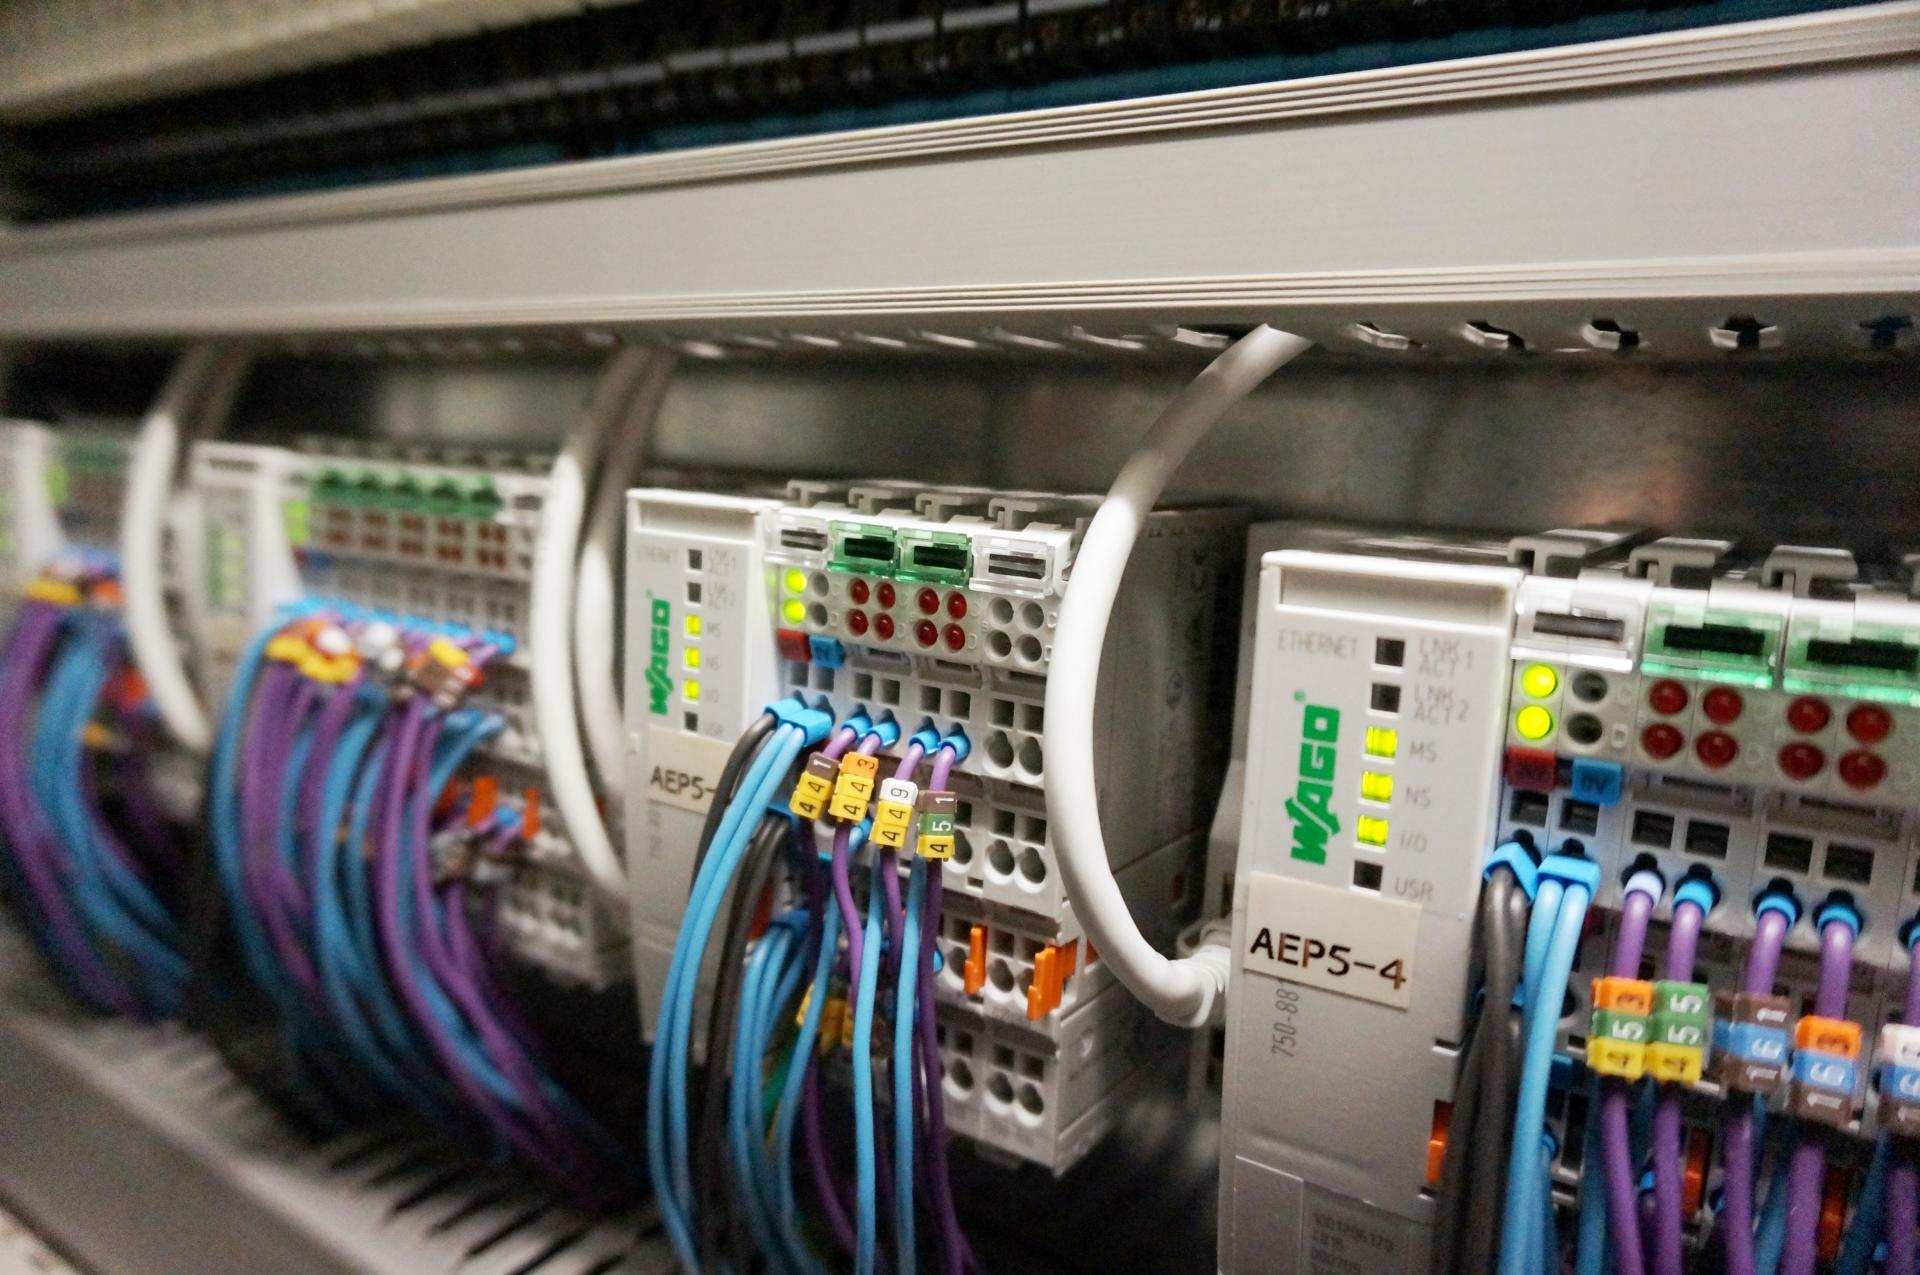
\includegraphics[width=0.7\textwidth]{data/plc.jpg}
\caption{Průmyslové \gls{plc} moduly. Převzato z~\texttt{wikimedia.org}.}
\label{fig:mtbusb-prototype}
\end{figure}

V~této práci se zaměříme na podmnožinu \gls{plc} modulů – totiž na takové,
jejichž hlavním úkolem je správně zpracovávat vstupní signály a~ovládat výstupní
periferie. Řízení logiky průmyslového procesu přenecháme počítači, s~kterým
\gls{plc} moduly komunikují.\footnote{V~praxi může \gls{plc} modul řídit logiku
procesu přímo, my však tuto situaci zkoumat nebudeme.}

Cílem této práce je navrhnout a implementovat novou verzi komunikační sběrnice
\gls{plc} obvodů \textit{\gls{mtbbus}} (\textit{Model Train
Bus}\footnote{Expanze zkratky do jejího plného významu nedává smysl, i~tak
budeme používat označení MTBbus, protože tak je zkratka zaužívaná.}).

\gls{mtbbus} je sběrnice, která se využívá pro řízení modelových kolejišť.
Je součástí systému \gls{mtb}. Skrze sběrnici lze číst signály z~kolejiště
(například polohy výhybek, obsazenost kolejových obvodů) a~povelovat prvky
v~kolejišti (návěstidla, přestavníky výhybek, přejezdy apod.). Obdobným
způsobem funguje zapezpečovací zařízení na skutečné železnici.

V~této práci autor nejprve popíše současné nasazení systému \gls{mtb}. Budou
formulovány důvody vedoucí k~nutnosti aktualizace sběrnice. Autor popíše, proč
jsou dostupná komerční řešení nevhodná a~navrhne vlastní nové (1) protokoly,
(2) hardwarové moduly a~(3) počítačové programy, které jím formulovaný problém
řeší.


\chapter{Současné nasazení sběrnice MTBbus} \label{chap:nasazeni}
Sběrnice \gls{mtbbus} vznikla okolo roku 2000, kdy se hledal vhodný systém pro
programovatelné počítačové řízení modelové železnice, spoluprací nadšenců
z~\textit{Klubu modelářů železnic Brno I} (dále jen \gls{kmz}) a \textit{Klubu
železničních modelářů Praha 3} \footnote{Je překvapivé, že
skupina nadšenců tehdy dokázala vytvořit systém, který by se mohl poměřovat se
současnými komerčními systémy řízení modelových kolejišť, viz dále.} \cite{mtb:web}.

\textit{Digital Command Control} (\gls{dcc}), dnes pravděpodobně
nejrozšířenější\footnotemark\\mezinárodně standardizovaný systém pro digitální
řízení modelové železnice \cite{dcc_intro:web} tehdy ještě nebyl v~České Republice
rozšířený. Navíc přirozeně vyvstal požadavek na minimalizaci nákladů
a maximalizaci nezávislosti na komerčních produktech jediného výrobce. Vznikl
tedy systém \gls{mtb}, který se pro řízení modelových kolejišť v \gls{kmz}
používá doteď \cite{kmz_rizeni:web}. Podotkněme, že systém \gls{mtb} se
do~dalších klubů po České Republice nerozšířil – nejspíš proto, že není
podporovaný komerčními softwary pro řízení modelové železnice a~že jej jeho
původní autor v~roce~2008 přestal podporovat.

\footnotetext{Autor této práce by rád odstranil slovo
\textit{pravděpodobně} a uvedl řádnou citaci. Bohužel neexistují studie, které
by bylo možné mohli citovat. Rozšířenost \gls{dcc} se zakládá na autorových
zkušenostech.}

\section{Popis sběrnice \gls{mtbbus}} \label{sec:mtbbus}

Každé kolejiště má svou vlastní sběrnici \gls{mtbbus}, ke které je připojený
právě jeden \textit{\gls{mtbusb} modul} a až \textit{255 \gls{mtb} modulů}.
\gls{mtbusb} modul řídí provoz sběrnice \gls{mtbbus} a~je připojen k~počítači.
\gls{mtb} moduly jsou pevně instalovány v~rámech kolejiště a~komunikují po
sběrnici \gls{mtbbus} s~\gls{mtbusb} modulem. Říkáme, že sběrnice je tzv.
\textit{single master, multiple slaves}. \gls{mtbusb} modul lze označit jako
\textit{master modul}, \gls{mtb} moduly jsou tzv. \textit{slave moduly}.
Celou situaci přehledně ilustruje obrázek \ref{fig:mtbbus-topology}.

Každý \gls{mtb} modul má:

\begin{compactenum}
\item 8bitovou adresu, která se konfiguruje \textit{jumpery} přímo na modulu,
\item konfiguraci (typ vstupů/výstupů, rychlost sběrnice, ...),
\item vstupy (stav vstupů),
\item výstupy (stav výstupů).
\end{compactenum}


\begin{figure}[ht]
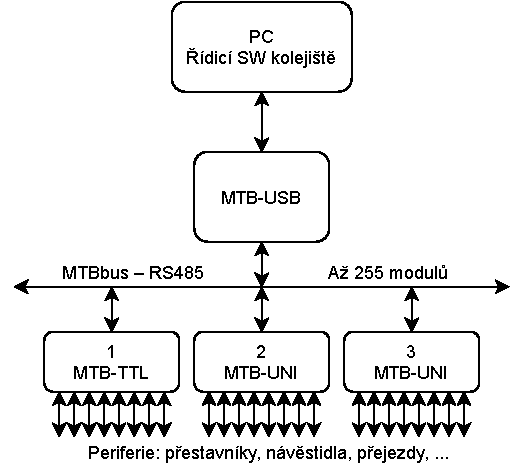
\includegraphics[width=0.7\textwidth]{data/mtb-topology.pdf}
\caption{Topologie systému \gls{mtb}.}
\label{fig:mtbbus-topology}
\end{figure}

\begin{table}[h]
	\begin{tabularx}{\textwidth}{XX}
		\toprule
		Typ přenosu & RS485, formát dat UART \\
		Komunikační rychlost & 38400~Bd, 57600~Bd, 115200~Bd \\
		Maximální počet modulů & 255 \\
		Počet datových bitů & 9 \\
		Stop bit & 1 \\
		Parita & žádná \\
		Maximální délka vedení & 100 m \\
		\bottomrule
	\end{tabularx}
	\caption{Základní parametry sběrnice \gls{mtbbus} \cite{mtbbus-specs}}
	\label{tab:mtbbus-params}
\end{table}

Současná sběrnice \gls{mtbbus} je založena na elektrickém standardu
\textit{RS485} \cite{mtbbus-specs}. Sběrnice RS485 je dvouvodičová (\textit{R+,
R-, GND}) vícebodová sériová poloduplexní komunikační průmyslová sběrnice
vyvinutá s~důrazem na odolnost vůči externímu rušení. Je vhodná pro přenos dat
na větší vzdálenosti, řádově až stovky metrů \cite{rs485-specs}. Pro dosažení
nejlepších elektrických vlastností by sběrnice měla být lineární. Sběrnice je
na obou koncích termínována rezistorem \textit{200 R} a~pull-up a~pull-down
rezistory pro držení definované úrovně signálu.

RS485 je velice snadno implementovatelná do prakticky všech mikrokontrolérů –
pro přístup ke sběrnici je třeba rozhraní UART, jeden pin pro řízení směru
komunikace a driver k~RS485.

\gls{mtb} moduly mohou být různého typu:

\begin{itemize}
\item \textbf{\gls{mtbuni}}

	\gls{mtbuni} (\textit{univerzální}) je nejpoužívanější typ modulu. Obsahuje
	16~digitálních vstupů a~16~digitálních výstupů. Na výstupech 0–7 umožňuje
	kódovat návěst protokolem S-COM\footnote{S-COM je jednoduchý jednosměrný
	komunikační protokol, který umožňuje přenášet návěsti návěstidel
	\cite{scom-specs}.}, což umožňuje připojení až 8 návěstidel k~jednomu
	\gls{mtbuni}. Modul dále umožňuje připojení IR čidel na
	vstupy\footnote{IR čidla jsou bodová čidla detekující průjezd vlaku, viz
	\ref{sec:ir}.}. Výstupy modulu jsou v~režimu otevřeného kolektoru
	s~maximální zátěží až 0.5~A~/~8~výstupů.

\item \textbf{MTB-TTL}

	\begin{figure}[ht]
	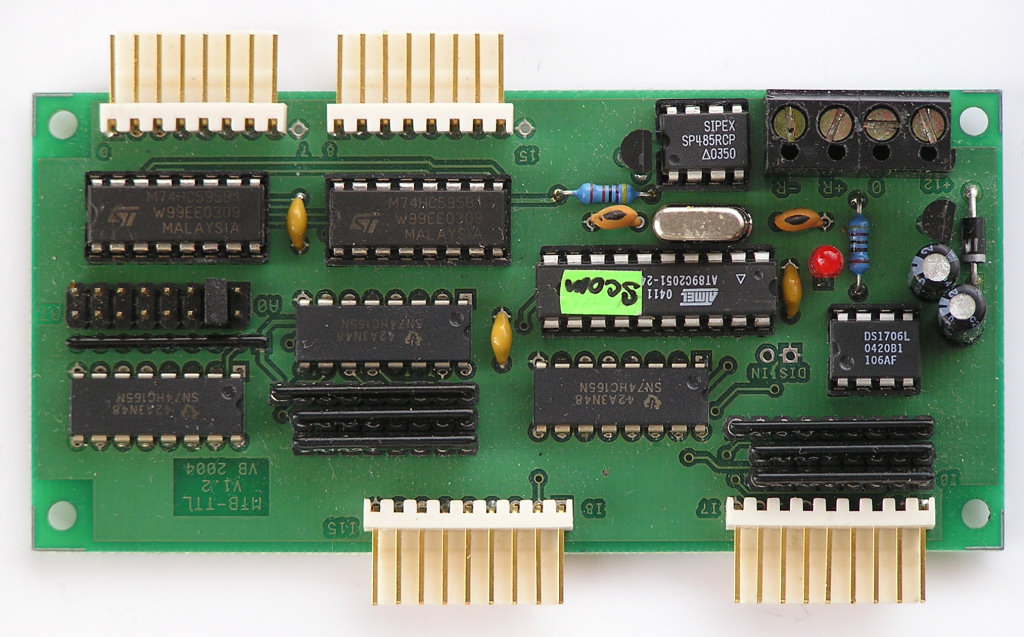
\includegraphics[width=0.7\textwidth]{data/mtbttl_foto.jpg}
	\caption{Ukázka modulu MTB-TTL \cite{mtb:web}.}
	\label{fig:mtbttl}
	\end{figure}

	MTB-TTL je zjednodušením modulu \gls{mtbuni}. Oproti \gls{mtbuni}
	nemá podporu IR čidel a~výstupy má v~režimu \gls{ttl}. Od tohoto typu
	modulu se v~současnosti ustupuje, neboť \gls{ttl} výstupy nejsou vhodné pro
	spínání vyšších napětí\footnote{např. pokud periferie na výstupu obashuje
	pull-up do +12~V} a~proto, že v~případě neaktivního výstupu (neaktivní =
	+5~V; inverzní logika) aktivně napájí výstupní port, což způsobuje nechtěné
	chování, například pokud je ne výstupním portu záměrně vypnutá periferie.
	V~krajním případě může dojít až k~přetížení TTL výstupu a jeho zničení. Na
	všechny nasazené moduly typu MTB-TTL byly postupně instalovány dodatečné
	obvody s~otevřenými kolektory na výstupy.

\item \textbf{MTB-REG}

	MTB-REG je modul umožňující generovat analogový výkonový výstup. Modul se
	připojí ke kolejím a řídí rychlost a~směr lokomotivy v~řízeném úseku kolejí.

	Tento způsob řízení jízdy (tzv. \textit{analogový}) je dnes již překonaný.
	V~současnosti se pro řízení jízdy lokomotiv na kolejišti používá tzv. systém
	\textit{Digital Command Control} (viz \ref{sec:dcc}), kde každá lokomotiva
	a mnohdy i~vagón v~sobě má mikroprocesor a~celý systém je řízen
	digitálně \cite{dcc_intro:web}.

	Modul MTB-REG je tedy již překonaným modulem a autor jej uvádí spíš pro
	úplnost popisu systému \gls{mtb}.

\item \textbf{MTB-POT}

	Modul MTB-POT obsahuje 4 analogové vstupy a 4 digitální vstupy. Jeho
	původním účelem bylo, aby se připojil k~potenciometru v~pultu obsluhy
	kolejiště, kterým obsluha reguluje jízdu vlaku. Po sběrnici přepošle data
	modulu MTB-REG a~tím dojde ke kýžené jízdě vlaku. Tento způsob řízení jízdy
	na kolejištích se již nepoužívá, proto i~modul MTB-POT na moderních
	kolejištích pozbývá svého smyslu.

\end{itemize}

Po sběrnici se komunikuje pevně definovaným protokolem.  Protokol definuje
příkazy pro moduly, odpovědi modulů, časování apod \cite{mtbbus-specs}.

Práce se sběrnicí z~pohledu aplikace v~počítači probíhá následovně:

\begin{compactenum}
\item Aplikace se připojí se k~MTB-USB modulu.
\item Aplikace provede sken aktivních modulů sběrnice.
\item Aplikace nahraje do všech aktivních modulů konfiguraci.
\item Aplikace přečte stav vstupů.
\item Aplikace zahájí provoz sběrnice – od této chvíle všechny moduly nahlašují
	změny stavů vstupů.
\item Aplikace čte vstupy, nastavuje výstupy a řídí provoz.
\item Aplikace ukončí provoz sběrnice a vynuluje stav výstupů \gls{mtb} modulů.
\item Aplikace uzavře spojení s~MTB-USB.
\end{compactenum}


\section{IR čidla} \label{sec:ir}

Nyní popíšeme princip fungování IR čidel v~kolejišti, protože bude v~dalších
kapitolách stěžejní.

IR čidlo je bodový detektor průjezdu vlaku. Do kolejí se vedle sebe umístí
opticky oddělená vysílací dioda a~fototranzistor, oba namířené vzhůru. Při
průjezdu vlaku dojde k~odrazu signálu od spodku vozu nebo lokomotivy, čímž je
detekován průjezd vlaku. Výhodou je nenápadná instalace mezi pražce, která
neruší celkový dojem modelu.

Pro spolehlivou detekci odrazu od matných černých povrchů podvozků je třeba
budit vysílací diodu vysokým proudem (až 200~mA), což vyžaduje použití
diody v~impulsním režimu. Současná \gls{mtbuni} deska podporuje IR čidla na
všech svých 16 vstupech, diody jsou buzeny tranzistory ve skupinách po
4~diodách.

\begin{figure}[ht]
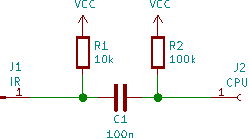
\includegraphics[width=0.5\textwidth]{data/cap-bind/capacitive-bind-example.pdf}
\caption{Zapojení vstupu kapacitní vazbou.}
\label{fig:cap-bind}
\end{figure}

Aby bylo zajištěno spolehlivé vyhodnocení odraženého signálu, je vstup
z~fototranzistoru zapojen na digitální vstup posuvného registru přes kapacitní
vazbu.

Vstupy \gls{mtbuni} desky se konfigurují osazením rezistorových lišt (běžný
vstup) nebo kondenzátorů (vstup z IR čidla). Kromě toho musí o~režimu pinu
vědět i~procesor, aby adekvátním způsobem zpracovával vstupní signál
\cite{mtbuni22-specs}.


\section{Systém \gls{mtb} v~kontextu řízení celého kolejiště} \label{sec:mtb_context}

V~\gls{kmz} je aktuálně systém \gls{mtb} nasazen na dvou kolejištích, další
nasazení je na modulovém kolejišti Mendelovy univerzity v~Brně, s~kterou klub
spolupracuje. Na těchto kolejištích je aktuálně nasazeno 99 \gls{mtb} desek.

Pro kontext uveďme, jak systém \gls{mtb} zapadá do celkové koncepce řízení
kolejiště. Viz schéma \ref{fig:control-topology}.

\begin{figure}[ht]
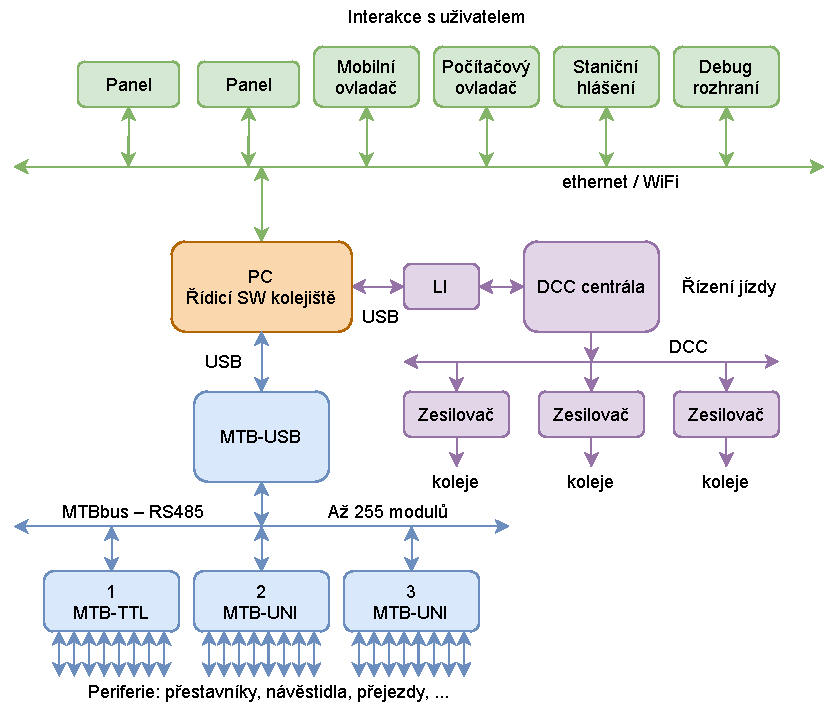
\includegraphics[width=\textwidth]{data/railroad-topology.pdf}
\caption{Schéma komponent řízení kolejiště v~\gls{kmz}.}
\label{fig:control-topology}
\end{figure}

Na první pohled je vidět, že kolejiště je řízeno dvěma různými systémy (modrá
a~fialová část diagramu).  Vyvstává otázka, proč je neintegrovat do systému
jednoho. Integrovaná řešení nabízejí majoritní výrobci hardwaru pro digitální
řízení modelové železnice.  Řízení jízdy i~trakce jedním systémem (\gls{dcc})
je rozšířeným přístupem jak v~Česku tak v~zahraničí. Všechna tato řešení jsou
však o~kompromisech, jak se dozvíme v~\ref{sec:dcc}. U~tvorby a~nasazení
systému \gls{mtb} stály osoby, které pracují na zabezpečení skutečné železnice.
Systém \gls{mtb} je tak oproti komerčně dostupným řešením řízení modelových
kolejišť navrhován s~důrazem na spolehlivost a~především bezpečnost.

Uveďme dva příklady za všechny: komerčně využívaná sběrnice RS pro snímání
stavu kolejiště nedokáže rozpoznat, že nějaký z~RS modulů (analogie \gls{mtb}
modulů) přestal fungovat \cite{rs:web}. Dále výstupní moduly nijak nepotvrzují,
že opravdu provedly akci, kterou počítač požaduje \cite{dcc_specs:web}. Tyto
příklady ilustrují, že komerčně dostupná řešení jsou podle autorova názoru blíže
hračce, než bezpečnému a~spolehlivému systému pro řízení modelů.

Poslední část schématu \ref{fig:control-topology} je část zelená, která
reprezentuje interakci s~uživatelem. \textit{Řídicí SW kolejiště} běží na
samostatném serveru, ke kterému se připojují všichni uživatelé systému –
dispečeři ze svých stanic, strojvedoucí ze svých ovladačů ale také třeba
technikové se svými diagnostickými nástroji nebo externí programy využívající
API serveru. Server kontroluje identitu uživatelů a umožňuje jim řídit ty
systémy, ke kterým mají uživatelé práva.

\section{Proč současný systém \gls{mtb} nedostačuje} \label{sec:mtb_fail}

Systém \gls{mtb} s~sebou nese řadu problémů.

\begin{enumerate}
\item \textbf{Licence, výrobní data}

U~současné implementace systému \gls{mtb} bohužel nebyly řádně vyřešeny licenční
podmínky mezi jeho autorem a~klubem. Souhrou událostí se \gls{kmz} dostal do
situace, kdy nemáme zdrojová data schémat a~layoutů desek plošných spojů ani
zdrojové kódy firmwarů.

Aktuální situace tak prakticky znemožňuje výrobu dalších \gls{mtb} desek,
o~záměru chtít systém \gls{mtb} nabízet mimo klub ani nemůže být řeč.

\item \textbf{Hardware}

Systém \gls{mtb} zaznamenal poslední aktualizaci hardwarových komponent v~roce
2007. V~současné době jsou některé použité součástky bohužel prakticky
nesehnatelné, což znemožňuje výstavbu dalších částí kolejiště. To je zcela
zásadní problém.

\item \textbf{Software}

Současné MTB moduly využívají procesory \textit{AT89C2051} (2~kB FLASH,
128~B SRAM). Tyto procesory svými parametry odpovídají době návrhu celého
systému. Firmware v~procesorech naráží na jejich hardwarové limity – do
procesoru se jednoduše nevejde další logika, což efektivně zabraňuje přidání
nových funkcí. Procesorům navíc chybí některé klíčové periferie, například
EEPROM paměť.

\end{enumerate}

Současný systém \gls{mtb} byl vyhodnocen jako celkově nedostatečný, je potřeba
ho buď aktualizovat nebo nahradit za systém jiný.

Na náhradu systému \gls{mtb} autor práce stanovil především následující
požadavky.

\begin{compactenum}
\item Systém musí být kompatibilní se současným řídicím softwarem kolejiště.
\item Systém musí být kompatibilní se současným hardwarem kolejiště.
\item Systém musí být udržitelný minimálně 20~let.
\item Finanční náklady a~čas vložený do povýšení současného systému na nový
	systém by měly být minimalizovány.
\item Systém musí být schopen potvrzovat akce řídicího počítače a~evidovat správnou
	funkčnost modulů.
\item Systém by měl být rozšiřitelný co se týče podporované funkcionality –
	nové požadavky na funkcionalitu by mělo být možné implementovat.
\end{compactenum}

K~naplnění těchto požadavků lze přistoupit dvěma různými způsoby: zakoupením
komerčního produktu nebo vytvořením produktu vlastního. Prozkoumejme nejprve,
jestli existují komerční řešení, která naplňují definované požadavky.


\chapter{Existující řešení} \label{chap:existujici-reseni}
Nyní představíme v~současnosti nejrozšířenější systémy pro \textit{digitální}
řízení modelové železnice. Prozkoumáme zařízení, která tyto standardy
podporují, a~zhodnotíme jejich vlastnosti. Bude vyhodnoceno, jestli zařízení
naplňují požadavky definované v~předchozí kapitole.

\section{Digital Command Control} \label{sec:dcc}

\textit{Digital Command control} (\gls{dcc}) je celosvětově nejrozšířenější
systém pro \textit{digitální}\footnote{\textit{Digitální} znamená, že mezi
jednotlivými prvky řízení proudí digitální data.} řízení modelové železnice
\cite{dcc_systems:web}. K~\gls{dcc} existují alternativy, které však v~Evropě
nejsou rozšířené, proto alternativní systémy nebudeme uvažovat.\footnote{Toto
tvrzení se zakládá na autorových zkušenostech, relevantní studie neexistují.}

\gls{dcc} specifikuje, které komponenty se účastní řízení kolejiště a jak se
tyto komponenty mají chovat – od elektrických standardů (např. doporučený
způsob zapojení vodičů pod kolejištěm) až po komunikační protokoly. \gls{dcc}
je otevřený standard vytvořený organizací \textit{National Model Railroad
Association} (\gls{nmra}), která sdružuje modelářské kluby (a~tedy i~modeláře),
které jsou přímými uživateli systému \gls{dcc}. Systém \gls{dcc} je tedy
navržen modeláři k~naplnění potřeb modelářů.

Jednotlivé prvky systému \gls{dcc} jsou znázorněny v~\ref{fig:dcc-overview}.
Nyní tyto prvky stručně popíšeme.

\begin{figure}[ht!]
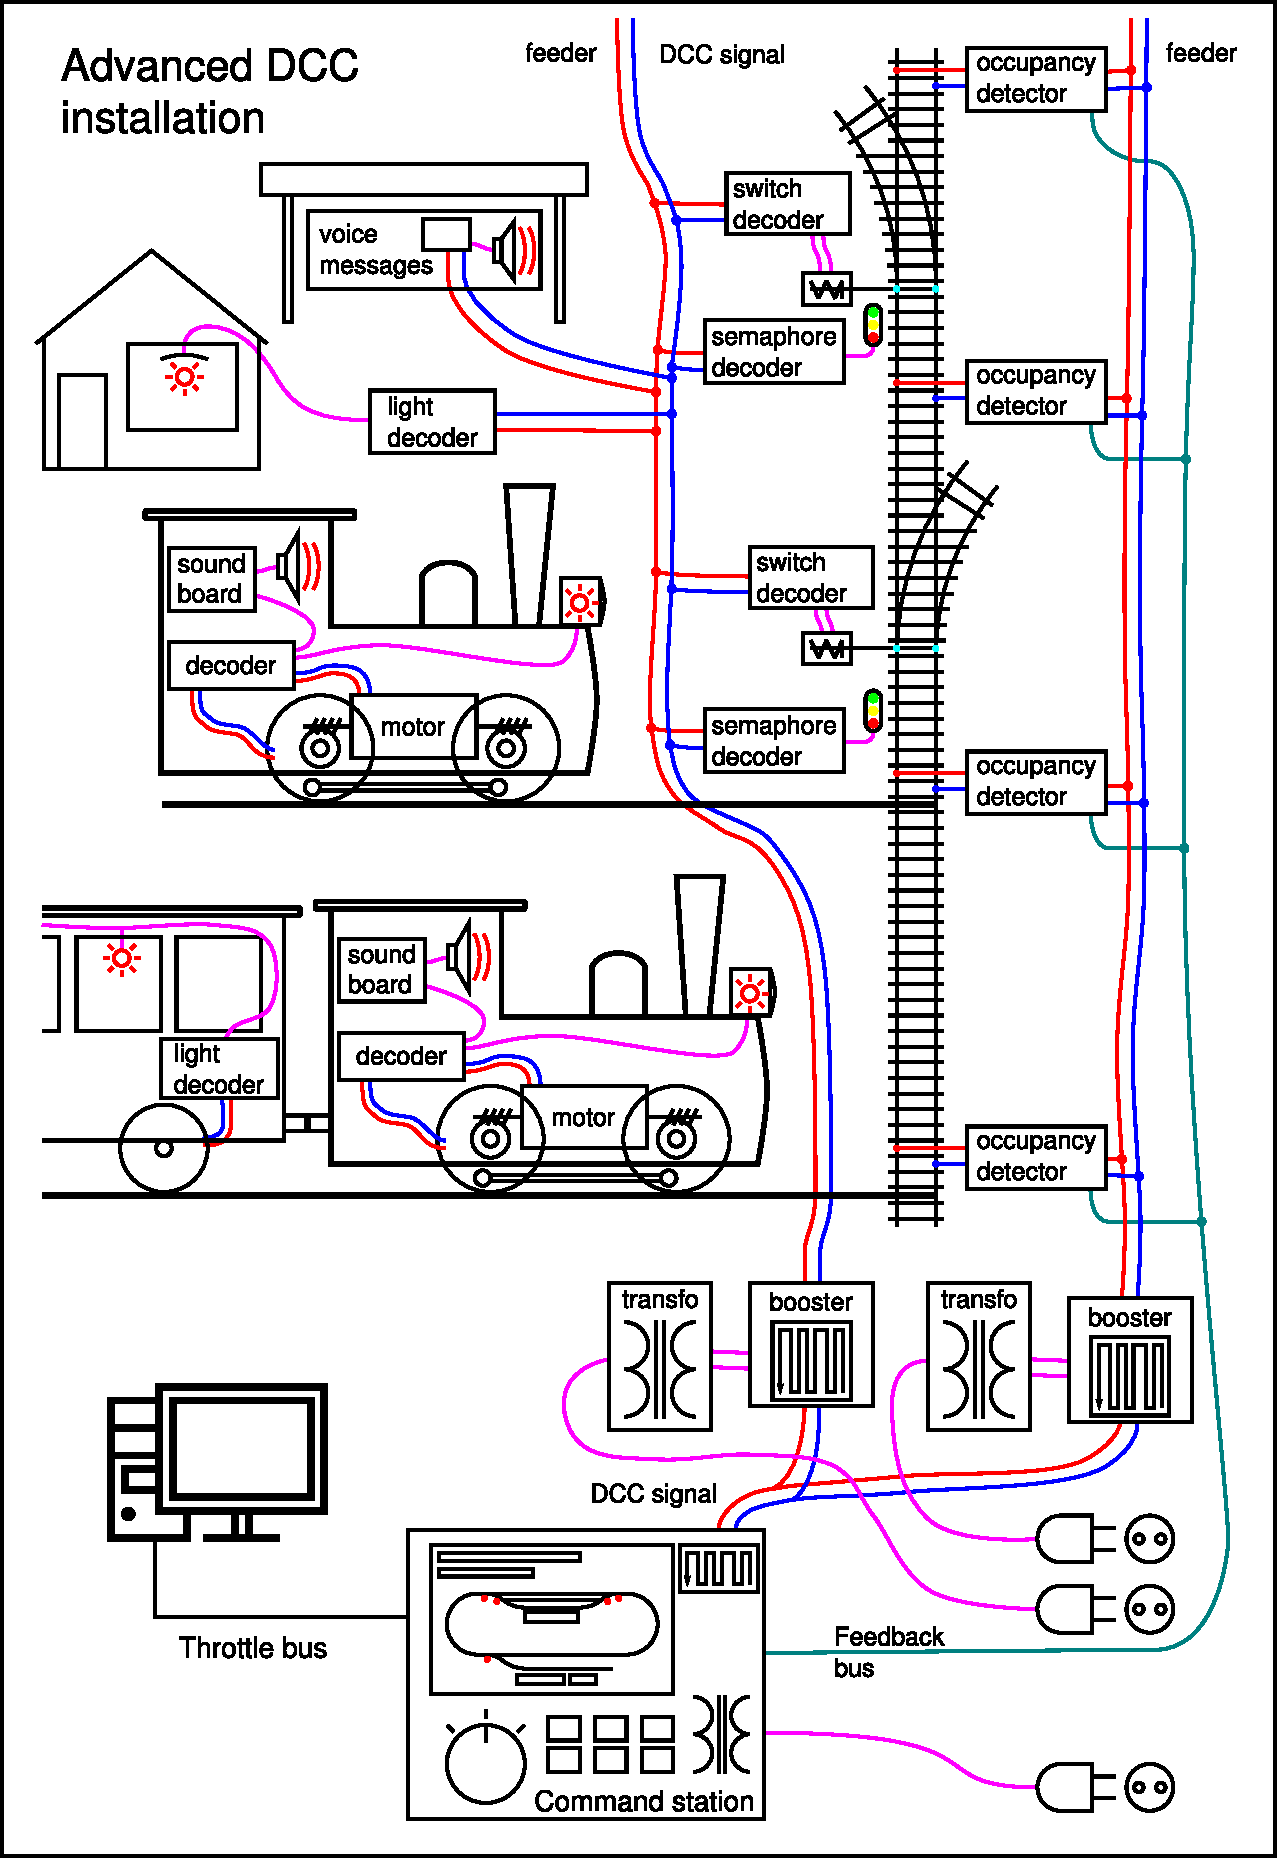
\includegraphics[width=0.95\textwidth]{data/schema_dcc_en.pdf}
\caption{Schéma systému \gls{dcc}. Převzato a upraveno z~\cite{dcc_wikipedia:web}.}
\label{fig:dcc-overview}
\end{figure}

Základní komponentou celého systému je \textit{DCC centrála (Command Station)},
která má 3 hlavní úkoly.

\begin{compactenum}
\item Číst stav \textit{modulů zpětného hlášení} přes \textit{sběrnici zpětného hlášení \\
	(feedback bus)}.
\item Povelovat \textit{dekodéry} (lokomotiv, přestavníků, návěstidel apod.).
\item Obousměrně komunikovat po \textit{sběrnici ovladačů (throttle bus)}.
\end{compactenum}

Řízení dekodérů centrála provádí generováním \textit{DCC signálu} (červený
a~bílý vodič ve schématu \ref{fig:dcc-overview}), do kterého centrála kóduje
operace požadované po dekodérech – např. \uv{dekodére číslo 541, zastav
lokomotivu}, \uv{dekodére číslo 4741, aktivuj čelní světla}.

Ke sběrnici ovladačů jsou připojené buď fyzické ovladače, nebo počítače.
Operátor provozu zadává příkazy, například otočením kolečka ovladače nebo
interakcí s~příslušným software, tyto příkazy jsou přeposlány do centrály,
centrála je dále přeposílá dekodérům, které přímo vykonávají požadované akce.

Na \textit{sběrnici zpětného hlášení} jsou připojeny moduly s~digitálními vstupy,
které jsou namontovány pevně v~kolejišti a~které čtou stav periferií.
Centrála informuje uživatele skrze \textit{sběrnici ovladačů} o~změnách ve
stavech vstupů \textit{modulů zpětného hlášení}. Vstupy modulů zpětného hlášení
jsou připojené například k~signalizacím obsazení \textit{kolejových obvodů},
takže uživatel nebo řídicí SW pozná, že se na koleji nachází nebo nenachází
vlak, dále například koncovým spínačům poloh výhybek, takže řídicí software je
schopen zabezpečit \textit{vlakovou cestu}.

Pro úplnost uvedeme všechny typy vstupů a~výstupů, které se v~\gls{kmz}
používají.

Výstupy:

\begin{compactitem}
\item řízení jízdy lokomotiv,
\item řízení osvětlení lokomotiv a vozů,
\item řízení zvuků lokomotiv,
\item nastavení polohy výhybky, výkolejky,
\item rozpojovač,
\item návěstidlo,
\item přejezd,
\item statické pouliční nebo domovní osvětlení,
\item indikace v~pultu obsluhy.
\end{compactitem}

Vstupy:

\begin{compactitem}
\item indikace obsazení kolejového obvodu,
\item indikace bodového průjezdu vlaku daným místem skrze infračervené čidlo
	(viz \ref{sec:ir}),
\item indikace koncové polohy výhybky,
\item indikace stavu přejezdu,
\item tlačítka v~pultu obsluhy.
\end{compactitem}

Všimněme si klíčové vlastnosti systému: pro řízení dekodérů
a~pro sběr informací z~kolejiště jsou použity 2~různé sběrnice: \textit{dcc
signál} a~\textit{sběrnice zpětného hlášení}. Platí totiž, že signál \gls{dcc}
je pouze jednosměrný. Signál putuje z~\gls{dcc} centrály přes
\textit{zesilovače} a přes koleje do lokomotiv a~vozů, které poveluje.
Existují jen velice omezené prostředky jak dostat data z~lokomotivy zpět do
\gls{dcc} centrály\footnote{Takovému systému říkáme \textit{RailCom}
\cite{railcom:web}.}. Tyto prostředky navíc vznikly až v~pozdějších verzích
normy \gls{dcc}, takže dnes nejsou všeobecně zaužívané \cite{railcom:web}.
Sběrnice \gls{dcc} je tedy prakticky vzato jednosměrná, dokonce bez odpovědí
dekodérů na příkazy

To znamená, že centrála musí DCC příkazy posílat opakovaně, aby zaručila, že je
dekodér skutečně přijme. Může se totiž snadno stát, že lokomotiva zrovna není
schopna přijímat signál – například jede po špinavých kolejích, ze kterých
špatně sbírá. Problém s~přijímáním dat vlivem špatného kontaktu se netýká
\textit{dekodérů příslušenství} (na obrázku \ref{fig:dcc-overview}
\textit{switch decoder} a \textit{semaphore decoder}).  Tyto dekodéry jsou
připojeny pevným kabelem ke kolejím, takže mají nejlepší předpoklady dekódovat
\gls{dcc} signál korektně. Stále však platí, že dekodér neodpoví, že přijal
a~provedl povel. Vykonání povelu mohlo být narušeno čímkoliv od
elektromagnetického rušení signálu až po nepřijetí povelu vlivem chyby ve
firmwaru dekodéru.

Může se zdát, že samotný protokol \gls{dcc} nesplňuje požadavky popsané
v~\ref{subsec:gen_requirements} a~proto jej nemá smysl uvažovat jako nástupce
současného systému \gls{mtb}. Ačkoliv striktně vzato je tento závěr
správný, je nutné si uvědomit širší souvislosti.

Pří řízení provozu na modelovém kolejišti sledujeme mnohé cíle, z~nichž na
prvním místě stojí bezpečnost. Na skutečné železnici je bezpečnost samozřejmě
mnohem důležitější než na železnici modelové. Přesto například materiální škody
vzniklé projetím návěsti zakazující jízdu, vykolejením soupravy, srážky nebo
následného pádu modelu na zem jsou tak markantní, že bezpečnost provozu je
třeba řešit.

Bezpečnost řízení provozu železnice skutečné i~modelové stojí na tom, že
nepustíme vlak do míst, kde by mu hrozila nehoda. K~nehodě může dojít dvěma
způsoby.

\begin{enumerate}
\item \textbf{Vlak stojí a~je nesprávně rozjet do místa, které pro něj není
bezpečné.}

	I~přes to, že dekodéry nepotvrzují přijetí signálu a~provedení akce, této
	situace se jsme schopni vyvarovat. Všechny klíčové komponenty kolejiště,
	které řídí směr pohybu vlaku (výhybky, výkolejky) indikují svůj stav. To
	znamená, že když se nepovede provést například přestavení výhybky vlivem
	nedoručení příslušného \textit{\gls{dcc} paketu}, výhybka se nepřestaví,
	moduly zpětného hlášení správně indikují, že výhybka se nehýbe, řídicí
	software správně vyhodnotí, že nedošlo ke splnění podmínek pro rozjetí
	vlaku a~vlak nerozjede.

	Z~tohoto pohledu tedy nepotvrzování \gls{dcc} příkazů nevede k~nebezpečné
	situaci.

	Jiná situace nastane u~dekodérů, které provádějí akce, aniž by indikovaly
	svůj stav. Takové dekodéry jsou například \textit{dekodéry návěstidel}
	(\textit{semaphore decoder} na obrázku \ref{fig:dcc-overview}). Tyto dekodéry
	však neovlivňují směr jízdy vlaku. Špatná návěst na návěstidle je
	nemodelová, ale ke hmotným ztrátám nedojde.
	\footnote{Jiná situace panuje na skutečné železnici, kde je návěst návěstidla
	důležitým komunikačním prvkem mezi dispečerem a~strojvedoucím. Je nutné,
	aby strojvedoucí viděl správnou návěst, protože nesprávná návěst
	by mu mohla povolit jízdu, přestože se například proti němu blíží vlak. Nebo
	by například mohla povolit jízdu vyšší rychlostí, než jaká je v~daném
	úseku předepsaná a~vlak by pak nemusel stihnout později zabrzdit. Proto se
	na skutečné železnici kontroluje, že světly návěstidel, která mají být
	rozsvícená, skutečně prochází proud.}

\item \textbf{Vlak se nepovede zastavit.}

	Může nastat situace, kdy se vlak blíží k~místu zastavení, řídicí software
	mu správně pošle příkaz k~zastavení, ale lokomotiva přesto nezastaví.
	Například vlivem již popsaného špatného kontaktu lokomotivy s~kolejemi
	a~tudíž neschopnosti řádně dekódovat \gls{dcc} signál. Norma \gls{dcc} totiž
	specifikuje \uv{pokud dekodér nedekóduje signál, zůstává ve stejném stavu}.
	Tedy například lokomotiva se pořád pohybuje vpřed.

	Popsaná situace v~praxi nastává, ale není v~záběru této práce s~ní naložit.
	Tato práce se zaměřuje především na řízení příslušenství a~snímání stavu
	kolejiště, nikoliv na systém řízení jízdy hnacích vozidel.

\end{enumerate}

Závěrem uveďme, že z~dosavadního popisu systému \gls{dcc} plyne, že tento
systém je pro řízení příslušenství vhodný, i~když s~drobnými nedokonalostmi.

\subsection{Sběrnice zpětného hlášení}

V~předchozí kapitole jsme při formulování závěrů vycházeli z~předpokladu, že
jsme schopni bezpečně indikovat stav všech prvků v~kolejišti (pomocí
\textit{sběrnice zpětného hlášení} – \textit{feedback bus} ve schématu
\ref{fig:dcc-overview}). Prozkoumejme spolehlivost této sběrnice.

\gls{nmra} nedefinuje jednotný standard pro \textit{sběrnici zpětného hlášení}
\cite{dcc_specs:web}, různí výrobci používají různé (vlastní) sběrnice
\cite{dcc_feedbacks:web}. Analyzujme nejpoužívanější sběrnice.

\subsubsection{S88}

\textit{S88} je základní sběrnice zpětného hlášení. Její fungování lze v~zásadě
charakterizovat jako \uv{vylepšené posuvné registry} \cite{s88:web}. Jednotlivé
moduly jsou řazeny za sebe, propojují se vždy sousední moduly. První modul je
připojen do \gls{dcc} centrály.

\begin{figure}[ht!]
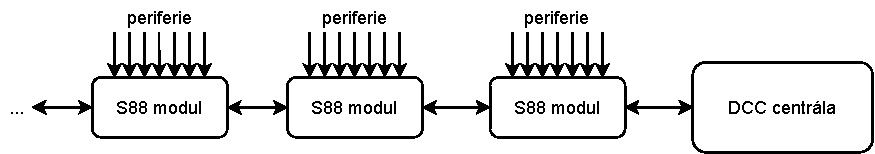
\includegraphics[width=\textwidth]{data/s88.pdf}
\caption{Topologie sběrnice S88.}
\label{fig:s88-topology}
\end{figure}

\textit{S88} je nízkonákladová sběrnice určená pro malá kolejiště. Limitujícím
faktorem je především napájení z~5~V, které není vhodné na delší rozvody,
a~malá odolnost proti rušení \cite{s88:web}.

Jak je patrné z~topologie sběrnice \ref{fig:s88-topology}, při výpadku
(napájení) jednoho modulu jsou ztracena data i~ze všech dalších modulů dále od
centrály. Takové chování je pro profesionální \gls{plc} systém nevhodné.

\subsubsection{RSbus}

\textit{RSbus} je sběrnice firmy \textit{Lenz Elektronik}. Oproti \textit{S88}
je organizována do topologie sběrnice. Jednotlivé moduly jsou napájeny
samostatně, sběrnice je dimenzovaná až na 128 modulů, každý s~8 digitálními
vstupy \cite{rs:web} \cite{rs_lib:web}.

\begin{figure}[ht!]
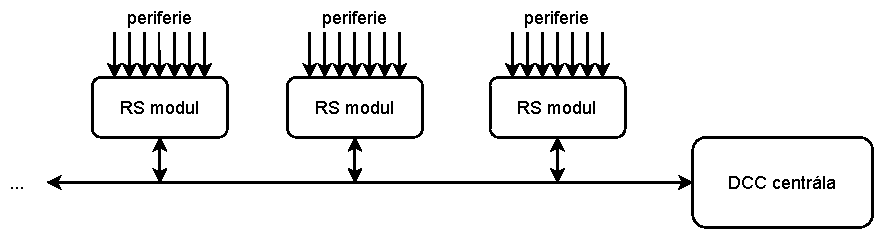
\includegraphics[width=\textwidth]{data/rs.pdf}
\caption{Topologic sběrnice RSbus.}
\label{fig:rs-topology}
\end{figure}

Komunikaci po sběrnici řídí \gls{dcc} centrála – posílá výzvy jednotlivým
modulům a~moduly odpovídají, pokud mají nějaká data k~odeslání. Moduly odesílají
data jen pokud došlo ke změně vstupů, což znamená, že nelze odlišit nefunkční
modul od funkčního modulu se setrvalým stavem vstupů \cite{rs_lib:web}.

Takové chování bohužel nesplňuje požadavky definované
v~\ref{subsec:gen_requirements}. Pokud by například došlo výpadku \textit{RS
modulu} a~následnému obsazení kolejového obvodu, jehož stav tento modul indikuje,
z~pohledu řídicího softwaru by byl kolejový obvod stále volný. Řídicí software
by pak povolil vjezd vlaku na obsazenou kolej, čímž by způsobil srážku.

K~výpadku RS modulu může dojít snadno například ztrátou napájení vlivem chybné
obsluhy, reakce pojistky na přetížení, poruchy apod.

\subsubsection{LocoNET}

Poslední z~analyzovaných sběrnic je \textit{LocoNET}. LocoNET je
proprietární sběrnice společnosti \textit{Digitrax} \cite{loconet:web}, jejíž
plná specifikace není volně dostupná \cite{loconet_license:web}.  Plné použití
této sběrnice podléhá licenčním poplatkům \cite{loconet_license:web}.
Zajímavou vlastností sběrnice je, že slučuje sběrnice \textit{throttle bus}
a~\textit{feedback bus} (viz schéma \ref{fig:dcc-overview}). Řídicí software
v~počítači tak může přímo dotazovat moduly zpětného hlášení a~úplně tak obejít
\gls{dcc} centrálu. Sběrnice LocoNET je navíc obousměrná,
LocoNET moduly jsou vstupně-výstupní, takže počítač může přímo
povelovat periferie \cite{loconet:web}. Viz \ref{fig:loconet-topology}.

\begin{figure}[ht!]
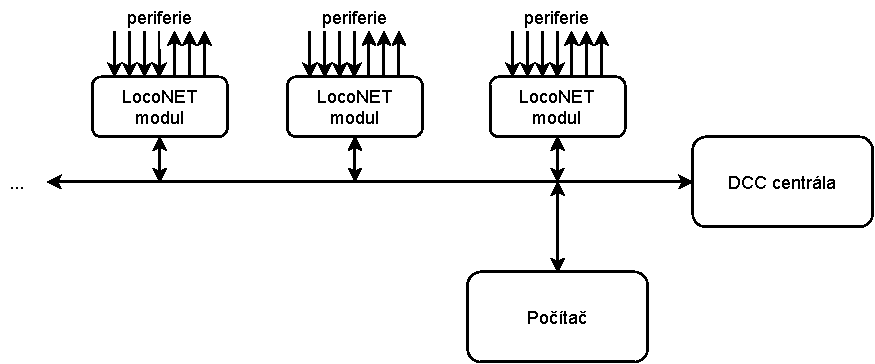
\includegraphics[width=\textwidth]{data/loconet.pdf}
\caption{Topologic sběrnice LocoNET.}
\label{fig:loconet-topology}
\end{figure}

Sběrnice LocoNET umožňuje počítači zjišťovat stav modulů přímou komunikací bez
zapojení centrály \cite{loconet-specs}, takže počítač může rozpoznat, které
moduly jsou na sběrnici přítomny, výpadek modulu a~oživení modulu po výpadku.

Sběrnice LocoNET splňuje požadavky na bezpečné řízení periferií
definované v~\ref{subsec:gen_requirements}. Při bližší inspekci však
zjišťujeme, že nasazení této sběrnice by znamenalo nakoupit a~vyměnit cca 100
modulů v~kolejišti. Výměna by navíc musela být rozsáhlejší, LocoNET
moduly přímo nepodporují například generování signálu \textit{\gls{scom}}. Pro
nasazení sběrnice LocoNET by musely být instalovány přídavné moduly
pro řízení návěstidel.

\section{BiDiB}

Zajímavou alternativou k~systému \gls{dcc} je sběrnice \textit{\gls{bidib}}
\footnote{\url{http://bidib.org/}} (\textit{BiDirectional Bus}). \gls{bidib}
je komunitní sběrnice s~otevřeným protokolem, která do velké míry splňuje
všechny požadavky definované v~\ref{subsec:gen_requirements}. Systém \gls{bidib}
lze provozovat na více komunikačních médiích (RS485, Ethernet, sériový port),
návrh systému je podobný návrhu \gls{usb} – na sběrnici je jeden \textit{master},
až 32 \textit{slave} v~každém segmentu, přičemž jedním ze \textit{slave} může
být \textit{hub} vedoucí do dalšího segmentu.

Autoři \gls{bidib} si dali za cíl, podobně jako autor této práce, vytvořit
bezpečný systém pro řízení modelových kolejišť. Systém tak podporuje potvrzování
příkazů, aktualizaci firmwaru modulů apod.

Pro nasazení \gls{bidib} by bylo třeba provést netriviální úpravy
aktuálních modulů kolejiště – \gls{bidib} například definuje standardní
konektory pro propojení modulů. Dále by bylo třeba vyřešit, jak naložit
s~limitem 32 desek v~jednom segmentu sběrnice (protože \gls{mtbbus} je navržen
až pro 255 modulů) a~s~jiným způsobem adresování modulů sběrnice.
\section{Závěr}

V~této kapitole byly popsány základní přístupy k~řízení moderní digitální
modelové železnice. Bylo zkoumáno, jestli komerční produkty splní požadavky
definované v~\ref{subsec:gen_requirements}. Po vyloučení technicky
nezpůsobilých řešení zbyly sběrnice LocoNET (s~poznámkou,
že její nasazení by bylo finančně náročné a~pracné) a \textit{\gls{bidib}}.

Při uvažování sběrnice LocoNET vyvstal problém s~integrací ovládání
návěstidel. Tento problém je obecnějšího rázu – jakékoliv komerční řešení není
schopné nabídnout takovou flexibilitu, jakou bychom v~\gls{kmz} potřebovali.
Je nutné integrovat systém řízení kolejiště se současnými periferiemi, ale
i~s~periferiemi budoucími. Je chtěné mít možnost pružně reagovat na nové
periferie, které se objeví například za 10 let.

Uvažme také aspekt zpětné kompatibility – vlastní systém nám umožní co možná
nejrozumněji zachovat kompatibilitu se stávajícím systémem řízení kolejiště
a~minimalizovat tak finanční náklady a čas nutný pro aktualizaci systému.
Nutnost rozumné zpětné kompatibility tak fakticky vylučuje i~nasazení
\gls{bidib}.

Vnímejme tuto kapitolu tedy především jako přehled technologií, které se
při řízení současné digitální modelové železnice používají. Přistupme k~návrhu,
jak povýšit systém \gls{mtb} výrobou vlastních komponent.


\chapter{Návrh MTB v4} \label{chap:mtb-v4-design}
Našim základním cílem v této kapitole bude navrhnout \gls{plc} systém, který
splňuje požadavky definované na konci kapitoly \ref{chap:nasazeni}. Při návrhu
tohoto systému vyjdeme z přirozeného požadavku na minimální změny v aktuálním
harwaru a softwaru kolejiště. Navrhneme nový systém jako iteraci současného
systému \gls{mtb}. Tento systém pojmenujeme \textit{MTB v4}.

Nový systém vyřeší všechny problémy aktuální verze systému \gls{mtb} popsané
v kapitole \ref{chap:nasazeni}. Při návrhu vezmeme v potaz aktuální technologie
v oblasti \gls{plc} obvodů a zvážíme implementace těcht technolgií. Detailně
rozebereme současnou implementace protokolu \gls{mtbbus} a u každé položky
zvolíme, jestli a proč ji chceme zachovat.

\section{Podrobná specifikace požadavků}

Abychom byli schopni navrhnout MTB v4, musíme znát přesné požadavky na takový
systém. Nyní požadavky formulujeme, přičemž budeme klást důraz na vysvětlení
změn oproti současnému systému \gls{mtb}.

Zaměřme se nejprve po požadavky, které na systém \gls{mtb} kladou komponenty,
které tento systém používají.

\subsection{Periferie v kolejišti}

K \gls{mtb} se na straně kolejiště připojují jednotlivé vstupy a výstupy
popsané v kapitole \ref{chap:existujici-reseni}. Všechny v současnosti na
kolejišti používané vstupy jsou digitálního formátu (binární vstupy), výstupy
jsou buď digitální binární nebo S-COM \ref{scom}. S-COM výstupy jsou ve
skutečnosti digitální výstupy, do kterých MTB deska moduluje S-COM signál.
S-COM signál je jednoduchý pomalý signál, který lze s přehledem vytvářet běžným
výstupním pinem procesoru nebo posuvného registru.

Oproti současnému \gls{mtb} bychom nově chtěli podporovat \textit{kmitavý
výstup} s počítačově definovou frekvencí kmitání a pevnou střídou. Jednalo by
se o kmitání v řádu jednotek \textit{Hz}, využití tohoto typu výstupu je pro
indikace v pultech a rozpojovače \ref{rozp}. I toto je však z pohledu hardwaru
jednoduchý digitální výstup, pro přidání tohoto typu výstupu je třeba upravit
pouze komunikační protokol a software a firmware modulů.

Současné moduly \gls{mtbuni} umožňují výstupy typu S-COM pouze na pinech
0–7, což je omezení dané malou pamětí procesoru. Toto omezení by mělo
\textit{MTB v4} relaxovat a umožnit tak, aby každý výstup mohl být v jednom
z režimů

\begin{compactenum}
\item digitální,
\item S-COM,
\item kmitavý.
\end{compactenum}

Co se týče vstupně-výstupních požadavků, \textit{MTB v4} by si vystačilo pouze
s moduly typu \gls{mtbuni} \ref{uni}. Na kolejišti v současnosti není žádný
prvek, který by vyžadoval například analogový vstup, analogový výstup nebo např.
\textit{PWM} výstup. Na kolejištích se hojně používají servomotory, ale vždy
pro řízení dvoupolohových prvků: výhybka, výkolejka, mechanické návěstidlo.
Všechny tyto prvky k sobě mají řídicí elektroniku, která interaguje se systémem
\gls{mtb} pouze digitálními piny. Typicky stačí 2 digitální výstupy (pro
nastavení požadované polohy) a případně 2 digitální vstupy (pro detekci koncové
polohy).

Zmiňme na tomto místě, že neimplementace PWM výstupů do \gls{mtbuni} v4
desky je koncepčním rozhodnutím autora této práce. Autor práce razí přístup
\uv{ať jedna věc dělá jeden úkol a dělá ho dobře}. Místo návrhu všemocného
\gls{mtbuni} modulu, který za pár let bude umět i uvařit kávu, se autor
rozhodl vydat cestou univerzálního kompaktního snadno sériově vyrobitelného
modulu s prostými digitálními vstupy a výstupy.

Připomeňme, že \gls{mtbuni} desky umožňují speciální typ vstupů – IR vstupy,
viz sekci \ref{sec:uni_ir}. Tyto vstupy vyžadují další elektroniku navíc.
V nových \gls{mtbuni} v4 deskách bude podpora pro IR čidla zrušena ve jménu
předchozího odstavce. Bude navržena speciální deska pro buzení a vyhodnocování
stavu IR čidel, která se bude připojovat přímo k digitálním vstupům
\gls{mtbuni} desky. Ušetří se tak elektronika na \gls{mtbuni} deskách,
na kterých se IR vstupy nevyužívají, zjednoduší se návrh desky plošných spojů
a umožní se využít IR čidla i s jinými deskami, než MTB, např. pro přímou
indikaci v pultech. Jedna deska bude dělat jednu věc a bude ji dělat dobře.

Na současném kolejišti si tedy vystačím pouze s \gls{mtbuni} deskami, které
budou navíc ořezané o podporu IR čidel. Ačkoliv je toto tvrzení pravdivé, bylo
by neperspektivní si podporu jiných typů desek zavřít volbou nevhodného
protokolu. Nový protokol sběrnice \gls{mtbbus} by měl být navržený univerzálně
pro nejrůznější možné typu desek, které v budoucnu mohou přijít. Autor této
práce má již v záměru takové desky desky vytvořit, více se můžete dočíst
v budoucí kapitole \ref{todo}.

\subsection{Ovládání}

Dalším uživatelem systému \gls{mtb} je řídicí software kolejiště. Tento
software je aktuálně na programován pro operační systém Windows a s hardwarem
kolejiště komunikuje pomocí dynamicky linkované knihovny, která musí dodržet
specifikované API \cite{api}. Na straně softwaru máme tedy relativně volné
ruce.

Princip řízení kolejiště dává požadavek na organizaci \gls{mtbbus} v4 sběrnice:
jednotlivé prvky jsou řízeny počítačem a výhradně počítačem.

Novým požadavkem je, aby v počítači mohlo existovat více softwarů, které
sběrnici řídí. V praxi totiž nastává kdy na jednu sběrnici jsou připojené systémy,
které mají být z principu řízeny různými programy: například zabezpečení řízení
provozu kolejiště a řízení pouličního a domovního osvětlení. Je vhodné mít oba
systémy zapojené do jedné sběrnice, aby se minimalizoval počet modulů, zejména
proto, že výstupů na řízení osvětlení je oproti řízení zabezpečení provozu málo.
Dává však také smysl, aby software pro řízení provozu neřídil osvětlení, protože
to není jeho účel.

Dalším reálným příkladem z \gls{kmz} je jedna sběrnice, na které jsou připojeny
periferie řízení tramvajové dopravy zároveň s periferiemi řízení silniční
dopravy. Přestože oba systémy sdíli společnou sběrnici, na úrovni počítače by
tyto systémy měly řídit dva různé programy. Jednom z hlavních přidaných hodnot
návrhu nového systému MTB je, že umožní \textit{multi-mater} řízení.

\subsection{Další požadavky}

Uveďme nyní některé méně důležité požadavky na novou verzi sběrnici \gls{mtbbus},
jejichž naplnění nám však výrazně zpříjemní její používání. Již teď předejímáme,
že všechny tyto požadavky se v implementaci podařilo naplnit.

\begin{enumerate}
\item \textbf{Umožnit nalezení \gls{mtb} modulů i po startu sběrnice.}

	V kapitole \ref{sec:mtbbus} byl popsán poměrně striktní proces používání
	sběrnice – od vyhledání modulů až po ukončení práce se sběrnicí. Současná
	implementace tohoto procesu neumožňuje, aby počítač detekoval moduly, které
	na sběrnici přibudou za jejího chodu. Taková situace může nastat například
	tak, že je prvně zapnut řídicí počítač a až pak napájení sběrnice. Je
	nepříjemné muset v takovém případě manuálně spouštět proces skenování
	znovu.

	Obecně se celý postup práce se sběrnicí popsaný v kapitole \ref{sec:mtbbus}
	zdá být příliš striktním. \gls{mtb} v4 by mělo tento proces zjednodušit.

\item \textbf{Z počítače bude možné na každém modulu zapnout identifikační LED.}

	Pro snadnou identifikaci konkrétního modulu v kolejišti, například při
	diagnostice závady, by operátor měl mít možnost na libovolném modulu
	zapnout indikační LED. Při diagnostice pod kolejištěm tak snadno identifikuje
	konkrétní modul.

\item \textbf{Firmware \gls{mtb} modulů by mělo být možné aktualizovat přímo
	po sběrnici \gls{mtbbus}.}

	Pod kolejištěm jsou nasazeny vyšší desítky modulů. Aktualizace jejich
	firmwaru ručním programováním všech modulů by byla časově náročná. Sběrnice
	by měla umožňovat aktualizaci firmwaru modulů přímo, ideálně za současného
	plného chodu zbytku modulů.

\end{enumerate}

\subsection{Shrnutí požadavků} \label{sub:mtbbus-req-summary}

Shrňme stručně všechny požadavky na systém \gls{mtb} v4.

\begin{compactenum}
\item K \gls{mtb} v4 se musí na straně počítače dát přistoupit skrze hJOP RCS
	API \cite{}.
\item V počítači může běžet více softwarů řídících výstupy a snímajících vstupy
	modulů sběrnice \gls{mtbbus} v4.
\item Systém \gls{mtb} v4 musí být navržený univerzálně pro nejrůznější typy
	modulů. Jedinou společnou vlastností modulů je, že snímají vstupy a nastavují
	výstupy.
\item Je třeba vyřešit zpětnou kompatibilitu především se stávajícími
	\gls{mtbuni} deskami v kolejišti.
\item Celé řešení by mělo být psáno opensource a openhardware, aby se dalo volně
	využívat.
\item Desky sběrnice \gls{mtbbus} v4 by mělo být možné průběžně vyhledávat,
	a detekovat nefunkční.
\item Implementace systému by měla využívat osvědčené komponenty, u nichž
	je dlouhodobý výhled dostupnosti.
\item Desky \gls{mtb} potvrzují příkazy, lze monitorovat jejich správnou funkčnost.
\item Z počítače bude možné na každém modulu zapnout identifikační LED.
\item Moduly \gls{mtbuni} budou nově podporovat kmitavé výstupy.
\item Moduly \gls{mtbuni} budou nově podporovat S-COM výstupy na všech pinech.
\end{compactenum}


\section{Návrh systému MTB v4}

Nyní provedeme návrh nového systému pro sběr dat z kolejiště a ovládání
periferií kolejiště. Detailně zdůvodníme každý aspekt nově navrhnutého systému.

\subsection{Vysokoúrovňový návrh}

Zachováme základní koncept fungování systému \gls{mtb} \uv{single master,
multiple slaves}. Vytvoříme novou verzi modulu \textit{MTB-USB}, který bude
jako jediný řídicím prvkem nové sběrnice \gls{mtbbus} v4. Model \textit{single
master, multiple slaves} je osvědčeným modelem, který se snadno implementuje,
lze snadno spočítat nejlepší a nejhorší časy odezvy sběrnice a obecně se dobře
mapuje na problém, který systémem \gls{mtb} chceme řešit.

Vytvořením nové verze modulu \textit{MTB-USB} sledujeme především to, aby
existovala svobodná implementace této desky, nová deska nám dále umožní využívat
moderních procesorů a integrovaných obvodů, které nám usnadní implementaci.
Tuto desku si můžeme dovolit vytvořit úplně novou, protože je pouze jedna
pro celé kolejiště. Malé počty desek implikují malé náklady na aktualizaci
sběrnice, což je přesně to, co chceme.

Navrhneme novou \textit{MTB-USB} desku, která bude splňovat všechny požadavky
definované výše a která bude založena na moderních, ale dlouhodobě dostupných
součástkách.

Nebudeme však vynucovat výměnu všech stávajících \gls{mtbuni} desek v
kolejišti. Provedeme výměnu procesoru v současné \gls{mtbuni} desce za
procesor nový a umožníme tak starým deskám fungovat na nové sběrnici. Tím se
minimalizují náklady na povýšení sběrnice.

Navrhneme IR desku, která bude zajišťovat podporu IR čidel, protože nová
\gls{mtbuni} deska již nebude obsahovat přímou podporu IR čidel.

Zachování většiny stávajícího hardwaru současných \gls{mtbuni} a snaha o
zachování kabeláže sběrnice s sebou nese ponechání volby sběrnice \gls{mtbbus}
na standardu RS485. RS485 nepřináší žádné zjevné nevýhody, takže není důvod,
proč hardwarovou vrstvu komunikační sběrnice měnit.

Nové procesory v \gls{mtb} modulech umožní trvalé uložení konfigurace v modulech.
Přesto bude autoritativním zdrojem konfigurace modulů i nadále počítač: po
nalezení modulu na sběrnici počítač tento modul zkonfiguruje dle konfiguračního
souboru. Tento přístup volíme proto, abychom byli schopni konfiguraci všech
desek kolejiště centralizovaně ukládat a verzovat.\footnote{Uložení konfigurace
v modulech i tak má smysl – například aby modul mohl aplikovat uložený bezpečný
stav výstupů přímo při zapnutí napájení modulu a nemusel čekat na zapnutí
řídicího SW v počítači.}

\gls{mtb} moduly budou skrze desku \textit{MTB-USB} komunikovat s počítačem
po portu USB, kterým bude tunelován \textit{USB CDC} protokol. V počítači tak
bude celá sběrnice přístupná skrze sériový port. Počítač nemůže komunikovat
po sběrnici RS485 přímo, protože na to nemá hardwarové periferie, proto bude
komunikovat s modulem \textit{MTB-USB}, který bude řešit časově kritické operace
sběrnice \gls{mtbbus}. \footnote{TODO popsat?}

Otázkou zůstává, kde naplníme požadavek na \textit{multi-master} řízení celého
systému. Existují v zásadě 2 možné přístupy:

\begin{compactenum}
\item \textit{MTB-USB} deska se bude k počítači připojovat rozhraním, které
	nativně umožňuje komunikaci pouze s jednou aplikací (např. USB) a řízení více
	programy se bude řešit na úrovni softwaru v počítači.
\item \textit{MTB-USB} deska se připojí k počítači rozhraním, které přirozeně
	podporuje více připojených zařízení, například ethernet.
\end{compactenum}

Oba přístupy se v komerčních systémech pro digitální řízení modelové železnice
používají. Ať bude podpora více řídicích systému implementována kdekoliv, oproti
jednomu řídicímu systému vyžaduje tato podpora netriviální programovou podporu
navíc. Autor práce se rozhodl přesunout co nejvíce složitější logiky do počítačových
aplikací, protože se ty se mnohem snáze vyvíjejí, ladí a aktualizují než firmware
v embedded procesorech. V počítači můžeme navíc využívat vysokoúrovňovější
nástroje. Vydáme se tedy cestou, kdy se deska \textit{MTB-USB} bude v k počítači
připojovat již pomocí zmíněného virtuálního sériového portu. V počítači
naprogramujeme novou aplikaci \textit{MTB Daemon}, která se na jedné straně
připojí k \textit{MTB-USB} modulu a na straně druhé vystaví JSON TCP server
s jednoduchým API, které umožní povelovat \gls{mtb} moduly z více počítačových
programů. Získáme tím mj. velice hezké programové API, ke kterému se bude dát
snadno připojit z knihoven nejrůznějších programovacích jazyků, a tím
zpřístupníme systém \gls{mtb} širšímu spektru programátorů.

Protokol CDC mezi počítačem a \textit{MTB-USB} deskou zvolíme proto, že se
jedná de fakto o standard pro připojení specifických periferií k počítači,
například v oblasti robotiky. S výhodou využijeme toho, že protokol CDC má
nativní podporu ovladačů snad v majoritních operačních systémech a není tak
nutné instalovat speciální ovladače. Tento aspekt nám umožní budoucí snadné
nasazení u externích zákazníků.

\subsection{\gls{mtbbus}}

Nyní podrobně rozebereme návrh nové sběrnice \gls{mtbbus}. Oficiální autorem
vytvořená plnohodnotná dokumentace nové sběrnice je k dispozici na
\url{https://github.com/kmzbrnoI/mtbbus-protocol}.

Požadavky definované v předchozích kapitolách vynucují razantní úpravy
komunikačního protokolu sběrnice. Autor této práce se rozhodl sběrnici
navrhnou celou od píky znovu. Sleduje tím především zajištění
\textit{přehlednosti} komunikačního protokolu sběrnice a také vyřešení potíží s
licencováním protokolu. Nový protokol je autorským dílem autora této práce
a tudíž si licenční podmínky může stanovovat sám.

\subsubsection{Hardware}

Jak již bylo zmíněno v předchozí sekci, po hardwarové stránce bude zachován
standard \textit{RS485} \cite{rs485}. Počet komunikačních bitů bude ponechán na 9.
Devátý bit ve zprávách z master to slave desky indikuje, že se jedná o první
byte zprávy. Ostatní bytes zprávy mají tento bit nastavený na 0. Devítibitová
komunikace nám umožní na sběrnici zavést klíčový pojem \textit{zprávy}. Díky
devátému bitu slave modul dokáže poznat, kdy zpráva začíná. Počet stop bitů
ponecháme standardně na jednom bitu, paritní bit nepoužijeme.

Aktuální specifikace sběrnice \gls{mtbbus} podporuje různé rychlost sběrnice –
38400 Bd, 57600 Bd a 115200 Bd. Komunikace vždy začíná na 38400 Bd a jeden
z prvních příkazů je příkaz na změnu rychlost sběrnice. Při výpadků a opětovném
oživení modulu musí modul postupně vyzkoušet ony 3 rychlost a sledovat, na které
rychlosti přijímá korektní data.

Možnost různých rychlostí by autor chtěl ponechat – některé kolejiště se
spletitou sběrnicí, dlouhou sběrnicí nebo sběrnicí se špatnými elektrickými
vlastnostmi mohou vyžadovat nižší rychlosti. Rchlost nižší než 38400 Bd by
neměla být třeba – tuto. rychlost by měla zvládat každá sběrnice. Při rychlosti
115200 Bd dojde průměrně k 10 skenům jednoho modulu při počtu 50 modulů.
Tato hodnota je poměrně malá, ale pro účely zabezpečovacího softwaru kolejiště
dostatečná. V budoucnu možná dojde k dalšímu zvýšení rychlosti sběrnice.


\subsubsection{Princip komunikace}

Sběrnice bude fungovat v režimu \textit{single master, multiple slaves}. Chod
na sběrnice bude řídit \textit{master} module – \textit{MTB-USB}. Master modul
bude periodicky dotazovat všechny moduly sběrnice s výjimkami zpráv pro konkrétní
moduly odeslané z počítače. Modul na každou zprávu pro něj odpoví právě jednou
zprávou. Proto není nutné ve směru \textit{slave $\rightarrow$ master} používat
devátý bit.

Modul na periodické výzvy o odpověď (\textit{Module Inquiry}) vždy odpoví daty
k odeslání. Pokud modul nemá žádná data k odeslání, odpoví zprávou
\textit{Acknowledgement}. Tím \textit{MTB-USB} modulu potvrdí, že zprávu přijal
a že komunikuje. \textit{MTB-USB} modul tka může monitorovat aktivní moduly
sběrnice a dokonce detekovat moduly nové.

Příklad komunikace po sběrnici:

\begin{verbatim}
> Module 1 Inquiry
< Acknowledgement  # Module 1 žije a nemá žádná data k odeslání
> Module 2 Inquiry
# Timeout – modul 2 nežije
> Module 3 Inquiry
< State of inputs changed, new state: 0b00001010 0b11110000
> Module 6 Inquiry
< Acknowledgement
> Change outputs of module 1 to 0b00101010 0b01000101
> Module 10 Inquiry
< Acknowledgement
...
\end{verbatim}

Všimněte si, že v příkladu probíhá polling pouze některých adres – pro zmenšení
latencí je vhodné často dotazovat aktivní moduly a neaktivní moduly skenovat
jen čas od času (aby se dalo poznat, že moduly ožily). Dále si všimněte, že
příkazy pro moduly chodí nezávisle na tom, která adresa je právě dotazována.

\subsubsection{Komunikační protokol} \label{subsub:mtbbus-proto-strucure}

Každá \textit{zpráva} má následující strukturu:

\begin{enumerate}
\item \textbf{Adresa modulu.}

Tento byte má jako jediný nastavený svůj 9. bit na hodnotu 1.
Adresa modulu je 8bitové číslo. Adresa 0 znamená, že příkaz se posílá
jako \textit{broadcast} a mají ho číst všechny moduly na sběrnici. Typickým
příkazem typu \textit{broadcast} je požadavek na reset výstupů všech modulů.

Adresní prostor 255 modulů byl vyhodnocen jako dostatečně velký.

\item \textbf{Délka zprávy.}

Tento byte obsahuje počet datových bytů zprávy plus jedna. Pro univerzálnost bylo
rozhodnuto protokol navrhnout tak, aby délka zpráv nebyla součástí definice
jednotlivých příkazů, ale aby byla ve zprávě obsažena explicitně. Toto
rozhodnutí umožňuje například \textit{MTB-USB} modulu přeposílat zprávy mezi
\gls{mtbbus} a počítačem, aniž by \textit{MTB-USB} muselo dekódovat obsah
zpráv, případně mít velkou tabulku \textit{typ zprávy, délka}. Některé zprávy
navíc mohou mít variabilní délku ze své podstaty.

Maximální hodnota tohoto bytu je 121, což umožňuje zprávy skládat do bufferů o
délce 128 bytes. Maximální délka zprávy byla zvolena s ohledem na nevelké
kapacity \textit{SRAM} mikrokontrolérů a časovou efektivitu případné
retransmise.

Původní verze protokolu \gls{mtbbus} umožňovala zprávy o délce nejvýše 7 bytů.
Tato hodnota byla zásadně navýšena zejména proto, aby bylo možné novým
protokolem posílat firmware pro aktualizaci \gls{mtb} desek.

\item \textbf{Kód příkazu}

Libovolné číslo v rozsahu 0–255. Význam jednotlivých kódů definuje specifikace
protokolu.

\item \textbf{Data příkazu}

Až 120 bytů.

\item \textbf{Kontrolní součet} (2 byty)

Kontrolní součet se ve zprávě uvádí, aby bylo možné ověřit integritu přijímané
zprávy. Integrita zprávy může být narušena například elektromagnetickým rušením
nebo špatnými elektrickými vlastnostmi přenosového média.

Původní protokol \gls{mtbbus} zabezpečoval integritu zprávy pomocí jednoduchého
mechanismu \texttt{xor}, kdy na jednotlivé byty zprávy byl aplikován bitový xor
a výsledná hodnota byla připojena na konec zprávy. Tento způsob je vhodný pro
malé zprávy.

Nová verze protokolu již umožňuje delší zprávy a tak byl navržen robustnější
způsob zabezpečení zprávy. Sběrnice \gls{mtbbus} v4 používá pro zabezpečení
zprávy mechanismus \textit{CRC-16} \cite{crc16-modbus}. Tento mechanismus je
založen na dělení polynomů se zbytkem. Konkrétně se používá verze
\texttt{CRC-16-IBM}, inspirací autorovi byla průmyslová sběrnice \textit{ModBus}
\cite{modbus}, která tento způsob zabezpečení zpráv používá také.

\end{enumerate}

Příklad zprávy: \texttt{0x101 0x001 0x001 0x091 0x090}.

\begin{compactenum}
\item \texttt{0x101}: zpráva pro modul s adresou 1.
\item \texttt{0x001}: následuje 1 byte zprávy.
\item \texttt{0x001}: příkaz \texttt{0x01}.
\item \texttt{0x091}, \texttt{0x090}: kontrolní byty \textit{CRC-16}.
\end{compactenum}

Zpráva neobsahuje žádná data příkazu.

\subsubsection{Zprávy} \label{subsub:mtbbus-messages}

Kompletní specifikace zpráv a jejich odpovědí je dostupná na
\url{https://github.com/kmzbrnoI/mtbbus-protocol}, zde uvedeme stručný přehled.

Zprávy master $\rightarrow$ slave:

\begin{compactitem}
\item \textit{Module Inquiry}
\item \textit{Module Information Request}
\item \textit{Set Configuration}
\item \textit{Get Configuration}
\item \textit{Beacon}
\item \textit{Get Input}
\item \textit{Set Output}
\item \textit{Reset Outputs}
\item \textit{Change Address}
\item \textit{Change Speed}
\item \textit{Firmware Upgrade Request}
\item \textit{Firmware Write Flash}
\item \textit{Firmware Write Flash Status Request}
\item \textit{Module-specific Command}
\item \textit{Reboot}

\end{compactitem}

Zprávy slave $\rightarrow$ master:

\begin{compactitem}
\item \textit{Acknowledgement}
\item \textit{Error}
\item \textit{Module Information}
\item \textit{Module Configuration}
\item \textit{Input Changed}
\item \textit{Input State}
\item \textit{Output Set}
\item \textit{Firmware Write Flash Status}
\item \textit{Module-specific command}
\end{compactitem}



Rozeberme nyní, proč zprávy vypadají tak, jak vypadají.

Jak již bylo zmíněno, \textit{MTB-USB} deska průběžně skenuje aktivní
i neaktivní moduly (aktivní častěji) a posílá modulům \textit{Module Inquiry}.
Moduly odpovídají buď \textit{Acknowledgement} nebo \textit{Input Changed}.

Zpráva \textit{Set Output} slouží k nastavení stavu výstupů modulu, zpráv
\textit{Reset Outputs} slouží k navrácení výstupů do bezpečného stavu.
Tato zpráva je typicky odesílána \textit{MTB-USB} modulem při ukončení komunikace
s počítačem jako broadcast.

Počítač může zapisovat nebo vyčítat konfiguraci modulů pomocí zpráv
\textit{Get Configuration}, \textit{Set Configuration} a odpovědi
\textit{Configuration}.

Počítač může zapínat a vypínat indikační LED na \gls{mtb} modulech pomocí
zprávy \textit{Beacon}.

Modulům, které si ukládají adresu softwarově, může operátor z počítače změnit
adresu pomocí zprávy \textit{Change Address}.

Plánovaná změna rychlosti sběrnice se modulům ohlašuje pomocí zprávy
\textit{Change Speed}, která je typicky odesílána jako broadcast. Každý modul
si ukládá rychlost sběrnice do volatilní paměti a tuto rychlost použije při
zapnutí. Očekává se, že budoucí typy procesorů v modulech \gls{mtb} budou
schopny detekovat rychlost sběrnice automaticky. Aktuálně není na sběrnici
\gls{mtbbus} implementován žádný mechanismus pro automatickou detekci rychlosti.
V situaci, kdy je například do sběrnice doplněn nový modul, který je ale z
výroby nastaven na jinou rychlost, než aktuálně sběrnice používá, se očekává,
že operátor přenastaví rychlost sběrnice na rychlost nového modulu, odešle
novému modulu příkaz na změnu rychlosti a vrátí rychlost sběrnice zpět.
Tento mechanismus je přímočarý a lze provést za plného chodu sběrnice.

Vysvětlení procesoru aktualizace firmwaru modulů se budeme věnovat v samostatné
kapitole.

Poslední zajímavou zprávou je \textit{Module-specific command}. Tato zpráva
umožňuje tunelovat pro modul libovolná data. Pokud typ modulu podporuje nějaké
speciální operace, může tento typ zprávy využít k řízení těchto operací.


\subsubsection{Dvouvrstvost protokolu}

Specifikace protokolu je tzv. \textit{dvouvrstvá}. Protokol specifikuje typy
zpráv, ale specifikace obsahu některých zpráv může být různá pro různé typy
modulů. Specifickými vlastnostmi modulů jsou:

\begin{enumerate}
\item Formát dat vstupů, formát dat výstupů

Protokol je navržený tak, aby moduly mohly mít libovolné vstupy i výstupy
i jejich počty. Obsah datových bytů zpráv \textit{Set Output}, \textit{Input
Changed} a \textit{Input State} je proto specifikovaný ve specifikaci modulů.

Například modul \gls{mtbuni} má 16 analogových a 16 digitálních výstupů.
Protože počet vstupů i výstupů je malý, posílá se v protokolu vždy celý stav
vstupů a výstupů. Protokol počítá s tím, že jiné moduly mohou mít vstupy a
výstupy například s větším rozsahem hodnot. V takovém případě protokol umožňuje
to, aby se neposílal celý stav vstupů a výstupů, ale jen relevantní část.
Například příkaz \textit{Set Output} může poslat jen ty výstupy, jejichž
stav je třeba změnit. To je také důvodem, proč existují 2 různé zprávy
\textit{Input Changed} (ve které se posílá jen stav změněných vstupů) a
\textit{Input State} (ve které se posílá stav všech vstupů).
\footnote{Všimněte si, že tento mechanismus umožňuje také provádět polling
vstupů místo událostního hlášení změn stavů vstupů. To je zcela záměrný prvek
protokolu. Tento prvek se využije například u budoucích modulů s analogovými
vstupy.}

\item Formát konfigurace

Konfigurace různých typů modulů se mohou zásadně lišit v počtu
konfigurovatelných hodnot.

Například modul \gls{mtbuni} ma 24 nebo 26 konfiguračních bytů
\ref{uni:proto}. Proto se celá konfigurace modulu posílá najednou.  Protokol
však umožňuje libovolný způsob zasílá konfigurace: počítač například u modulů s
větším množstvím konfigurace může poslat rozsah adres, jejichž hodnoty chce
znát. Nebo naopak poslat rozsah adres a hodnoty na těchto adresách, které
nastavuje.

\item Adresování a data paměti pro aktualizaci firmware

Různé typy modulů typicky obsahují různé procesory, které jinak adresují paměť.
Liší se například šířka slova nebo velikost paměti. Význam datových bytů
zpráv pracujících s aktualizací firmwaru procesoru je proto definován pro
konkrétní typy modulů.

\end{enumerate}

\subsubsection{Typické fungování sběrnice}

Následující kroky popisují typické fungování systému \gls{mtb} (srovnejte
s~postupem definovaným na konci \ref{sec:mtbbus}).

\begin{compactenum}
\item Je zapnut řídicí počítač kolejiště.
\item Je připojeno napájení \textit{MTB-USB} desky a všech \gls{mtb} modulů.
\item \gls{mtb} moduly z paměti načtou konfiguraci, aplikují bezpečný stav
výstupů, začnou poslouchat na sběrnici.
\item \textit{MTB-USB} deska detekuje připojené moduly a zapamatuje si je.
\item Počítačová aplikace se připojí k \textit{MTB-USB} desce.
\item Počítačová aplikace vyčte z \textit{MTB-USB} desky seznam aktivních modulů.
\item Aplikace vyčte typ připojených modulů, zkonfiguruje je.
\item Řídicí SW kolejiště používá sběrnici – čte vstupy, nastavuje výstupy.
\item Při odpojení řídicího SW kolejiště je \gls{mtb} modulům poslán příkaz
	k resetování stavu výstupů, čímž je zajištěno, že při odpojení nebo pádu
	řídicího softwaru se budou nacházet výstupy v definovaném stavu.
\end{compactenum}

Systém \gls{mtb} však nevyžaduje striktní pořadí těchto kroků. Napájení
komponent může být zapnuto v libovolném pořadí, systém dokáže detekovat výpadky
jednotlivých prvků a obnovovat je. Pro ilustraci uveďme několik příkladů situací,
které v systému \gls{mtb} mohou nastat.

\begin{itemize}
\item Jiné pořadí zapnutí prvků.

Pokud je \textit{MTB-USB} zapnut až po zapnutí počítače, počítač tento stav
korektně detekuje (chybí CDC USB zařízení) a po připojení \textit{MTB-USB} jej
korektně inicializuje.

Sken všech adres sběrnice \gls{mtbbus} (255 adres) probíhá neustále, takže
pokud jsou moduly sběrnice zapnuty až po zapnutí napájení \textit{MTB-USB} desky,
jsou i tak korektně detekovány.

\item Výpadek \gls{mtb} modulu.

Pokud \gls{mtb} modul neodpovídá na požadavky, \textit{MTB-USB} to detekuje, nahlásí
situaci do počítače a počítač se podle toho zachová.

Pokud \textit{MTB-USB} deska detekuje nový \gls{mtb} modul, opět o tom zpraví
počítač, ten provede vyčtení typu desky a zkonfiguruuje ji.

\item Výměna modulu za chodu sběrnice

Starý modul je při odpojení napájení nahlášen jako neaktivní, po výměně modulu
je aktivován nový modul.

\item Změna adresy modulu za chodu sběrnice

Původní adresa je prohlášena za neaktivní (neodpovídá na požadavky), nová adresa
je nalezena a zkonfigurována.

\end{itemize}


\subsubsection{Aktualizace firmwaru \gls{mtb} modulů}

Sběrnice \gls{mtbbus} je navržena tak, aby skrze ní mohl být aktualizován
firmware \gls{mtb} modulů. Při návrhu mechanismu aktualizace firmwaru bylo
zvažováno, jestli proces aktualizace firmwaru nevést úplně jiným protokolem,
než \gls{mtbbus}. \gls{mtbbus} Je dostatečně obecný a navíc je třeba, aby
při aktualizaci jednoho modulu ostatní moduly sběrnice aktualizační příkazy
ignorovaly a nerušily tak aktualizaci. Tyto argumenty vedly k implementaci
mechanismu aktualizace firmwaru přímo do sběrnice \gls{mtbbus}. Výhodou tohoto
řešení je, že zbylé moduly sběrnice mohou při aktualizaci firmwaru jednoho
modulu nadále komunikovat, aktualizace tedy může probíhat za plného provozu.

Protokol počítá s tím, že přepis flash paměti v \gls{mtb} deskách může
probíhat pouze z bootloaderu \gls{mtb} desky. Aktualizační protokol proto
podporuje reboot procesoru do bootloaderu. Procedůra aktualizace firmwaru
probíhá následovně \footnote{Procedůra je podrobně popsaná v dokumentaci protokolu
\gls{mtbbus} na
\url{https://github.com/kmzbrnoI/mtbbus-protocol/blob/master/workflows.md}.}.

\begin{compactenum}
\item Master deska vyšle \textit{Firmware Upgrade Request}. Tím informuje \gls{mtb}
	modul, že má rebootovat do bootloaderu.
\item \gls{mtb} deska odpoví \textit{Acknowldgement} a rebootuje do bootloaderu.
\item \gls{mtbusb} deska pošle \gls{mtb} desce žádost o její obecné informace.
\item \gls{mtb} deska odpoví obecnými informacemi, ve kterých je mj. zaznačeno,
	že je v bootloaderu.
\item \gls{mtbusb} deska vyšle příkaz \textit{Firmware Write Flash}, ve kterém pošle
	blok flash paměti k zapsání a její adresu. Slave deska tuto paměť zapisuje.
\item \gls{mtbusb} modul se ptá \gls{mtb} modulu příkazem \textit{Firmware Write
	Flash Status Request}, jestli již byl zápis dokončen. Jakmile je zápis bloku
	paměti dokončen, přesouvá se na krok (5).
\item Jakmile je zapsána celá paměť, master deska pošle příkaz \textit{Reboot},
	\gls{mtb} modul provede kontrolu konzistence paměti a zapne se do hlavního
	programu.
\end{compactenum}

Jak bylo zmíněno v posledním kroku, je doporučeno (a nový firmware
\gls{mtbuni} modulů toto doporučení dodržuje), aby při každém náběhu
procesoru modulu proběhla kontrola konzistence paměti. Kontrola konzistence
paměti je implementována pomocí uloženého kontrolního součtu (\textit{CRC-16})
na konkrétních adresách paměti. Protokol \gls{mtbbus} implementuje atribut,
kterým může \gls{mtb} modul oznámit, že sice poslouchá, ale je v bootloaderu
a odmítá nabootovat, protože nesedí kontrolní součet paměti programu.

Aktualizace bootloaderu přes sběrnici \gls{mtbbus} není možná, protože vlivem
výpadku napájení při aktualizaci programu by mohlo dojít k situaci, kdy se modul
stane nepoužitelným. Bootloader by měl být malý a odzkoušený kus firmwaru, který
se nahraje jednou a nikdy ho nebude třeba přehrávat. Přehrání bootloaderu by
vyžadovalo ruční obcházení modulů s programátorem.


\chapter{Implementace MTB v4} \label{chap:mtb-v4-impl}
\section{\gls{mtbusb} v4}

\begin{figure}[ht]
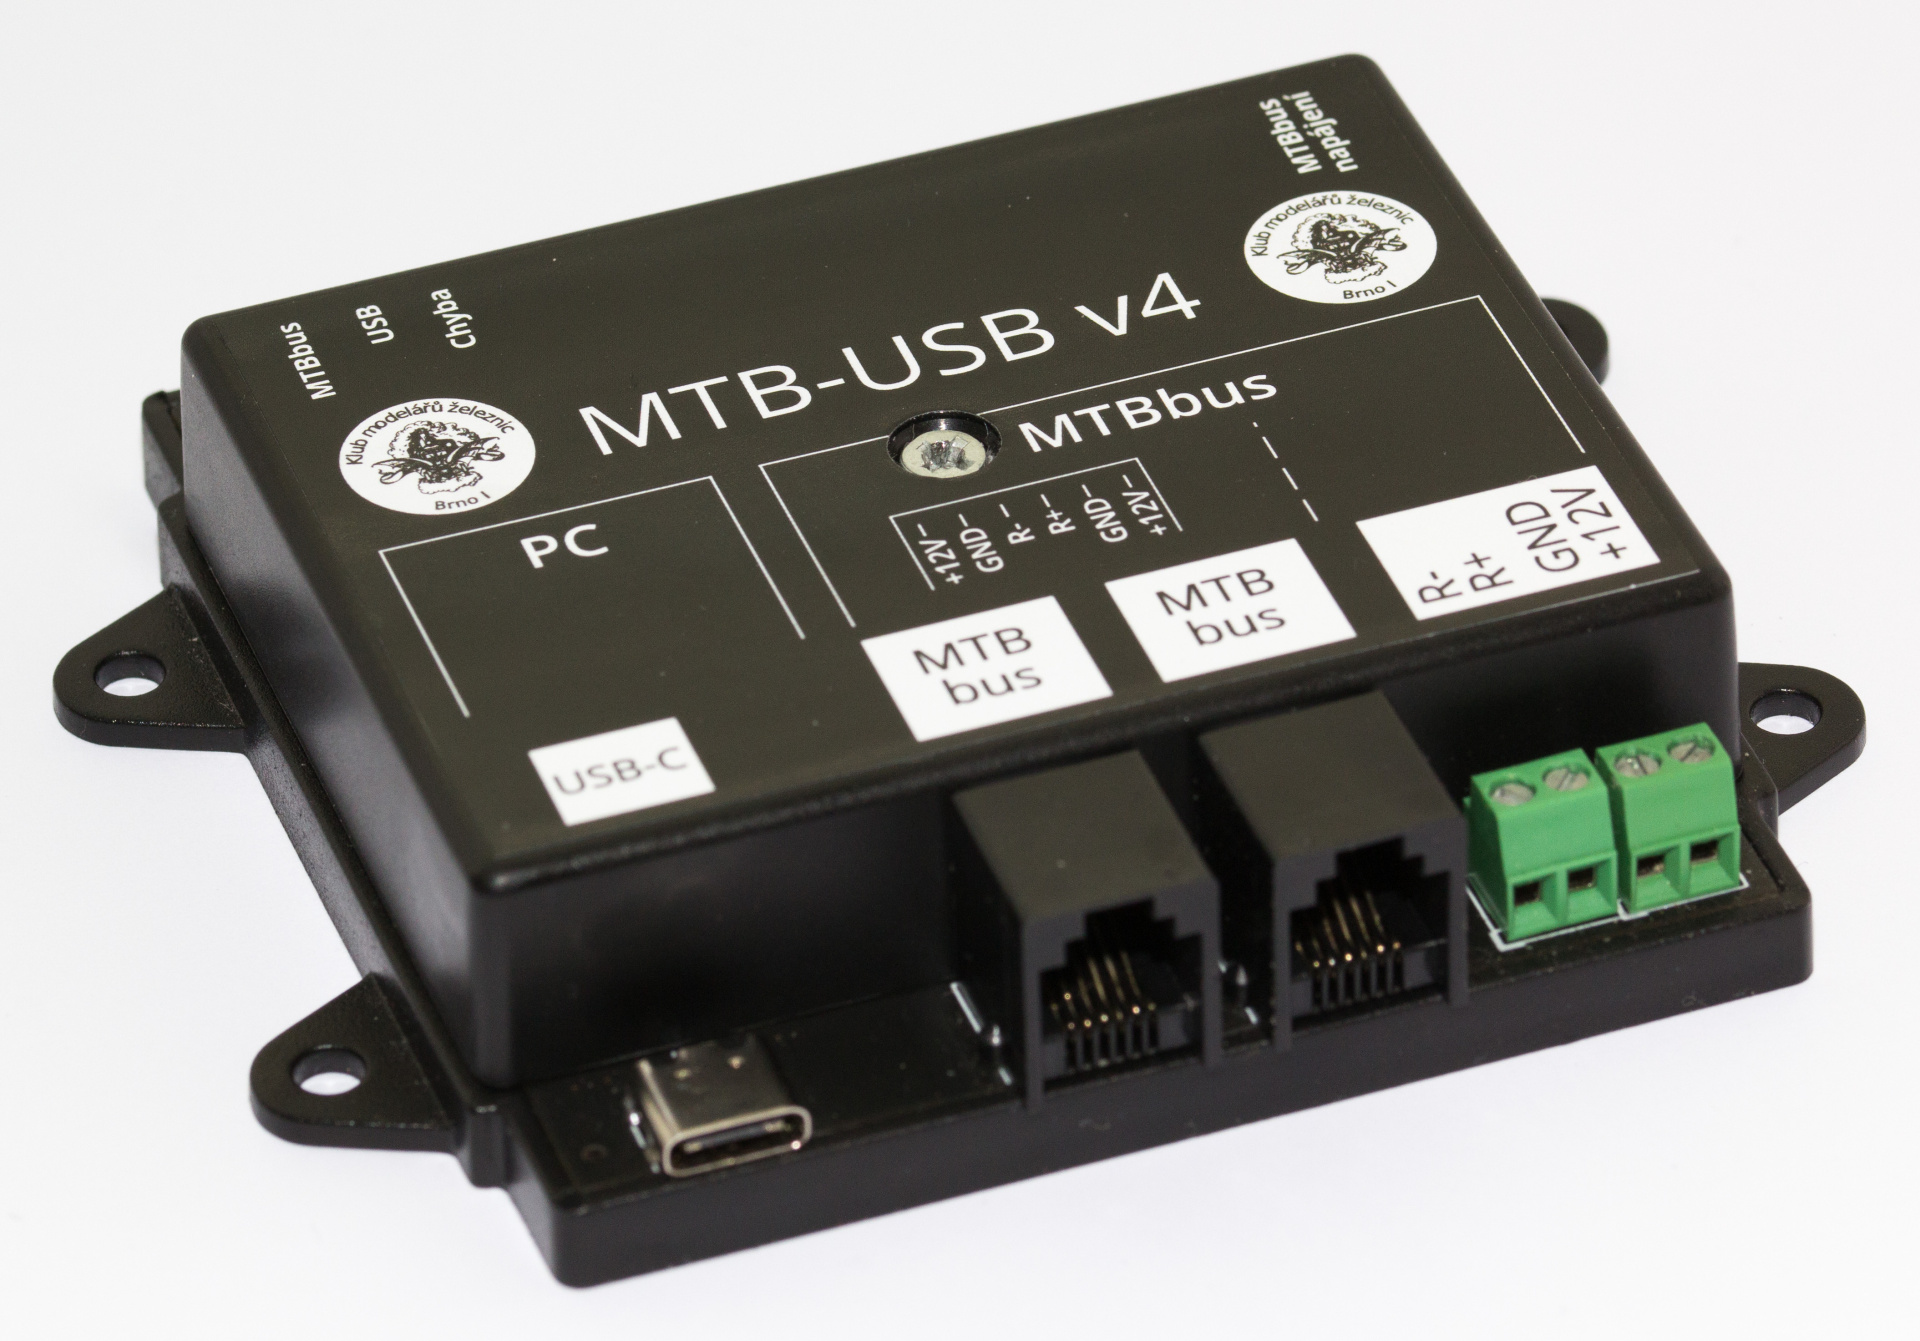
\includegraphics[width=0.7\textwidth]{data/usb-all.jpg}
\caption{Prototyp modulu MTB-USB.}
\label{fig:mtbusb-prototype}
\end{figure}

\gls{mtbusb} modul vzniknuvší v rámci této práce byl navržen kompletně nový,
inspirace starým \gls{mtbusb} modulem je minimální. Vznikly hardware, firmware
a popisy komunikačních protokolů.

Hlavním úkolem \gls{mtbusb} modulu je přeposílat data mezi sběrnici \gls{mtbbus}
a počítačem. \gls{mtbusb} modul provádí časově kritické operace sběrnice
 – například počítání timeoutu odpovědi na zprávu od \gls{mtb} modulů; pravidelné
dotazování \gls{mtb} modulů. Počítač pak informuje formou událostí.

\subsection{Komunikační protokol s počítačem}

Před návrhem samotné implementace je třeba navrhnout komunikační protokol
s počítačem. Tento komunikační protokol musí být přirozeně jiný, než nový
komunikační protokol sběrnice \gls{mtbbus}, který jsme popsali v předchozí
kapitole, protože zahrnuje jiné aktéry a funguje na jiné hardwarové platformě.

Komunikační protokol \gls{mtbusb} desky a počítače je navržen tak, aby byl do
velké míry nezávislý na protokolu sběrnice \gls{mtbbus}. Zásadním příkazem
je příkaz na přeposlání zprávy mezi \gls{usb} a \gls{mtbbus}. Tento příkaz umožňuje
počítačovému programu přeposlat libovolnou zprávu pro libovolný \gls{mtb} modul
(a naopak), aniž by \gls{mtbusb} deska musela znát sémantiku příkazů sběrnice
\gls{mtbbus}. Protokol sběrnice \gls{mtbbus} byl vytvářen přesně s tímto
cílem.

Na \gls{mtbusb} desku můžeme tedy pohlížet v zásadě jako na tenkého
přeposílatele mezi dvěma různými sběrnicemi – tzv. \textit{gateway}.

Plnohodnotná specifikace protokolu mezi počítačem a \gls{mtbusb} deskou je
k disopzici na \url{https://github.com/kmzbrnoI/mtbbus-protocol/tree/master/pc}.
Popišme nyní stručně návrh protokolu.

Mezi počítačem a \gls{mtbusb} deskou se komunikuje po virtuálním sériovém portu
(tzv. \textit{\gls{cdc}}) tunelovaným skrze \gls{usb} rozhraní. Toto řešení bylo vybráno,
protože je prakticky standardem pro připojením speciálních periferií k počítači.
Zvažován byl také například \textit{HID}. Samotná sběrnice \gls{usb}
nepodoporuje pojem zprávy tak, jak bychom ho vyžadovali\footnote{Při užití třídy \gls{cdc}
se data posílají nejčastěji každou milisekundu a to v bloku o nejvýše 64 bytech.
Počítačová aplikace díky bufferování operačního systému není schopna tyto bloky
spolehlivě rozlišit.}. Protože USB podporuje pouze 8bitový sériový port, začátek
zprávy je třeba označit jiným způsobem. v navrhovaném protokolu je začátek zprávy
označen speciální sekvencí dvou bytů \texttt{0x2A 0x42}. Tato sekvence se sice
ve zprávě může objevit, ale pravděpodobnost, že dojde k tolika chybám, aby
tato sekvence uprostřed zprávy byla považovaná za začátek zprávy, je
malá.\footnote{Uvědomme si, že rozdělování dat do zpráv na straně přijímače
se nemusí řídit jen detekcím magické sekvence bytů. Pokud zprávy nechodí moc
často, lze po delší době nepřijímání dat (třeba jednotky milisekund) vyprázdnit
vstupní buffer a očekávat, že další příchozivší data budou novou zprávou. Odesílací
strana nesmí odesílat jednotlivé části zprávy s velkou prodlevou, to je ale
rozumný požadavek.}

Celková struktura zprávy vypadá následovně (op jednotlivých bytech):

\begin{compactenum}
\item \texttt{0x2A},
\item \texttt{0x42},
\item počet následujících bytů,
\item kód příkazu,
\item data (až 122 bytů).
\end{compactenum}

Struktura je podobná struktuře zprávy protokolu \gls{mtbbus}, viz
\ref{subsub:mtbbus-proto-strucure}. Pozorný čtenář si přesto všimne například
chybějícího kontrolní součtu. Ten chybí, protože integritu zprávy řeší přímo
sběrnice \gls{usb} a tak ji není třeba řešit znovu. Upozorňujeme, že
\textit{kód příkazu} není kód příkazu sběrnice \gls{mtbbus}, ale kód příkazu
protokolu PC – \gls{mtbusb}.

Zprávy od počítače pro \gls{mtbusb} modul jsou:

\begin{itemize}
\item \textbf{Forward packet to \gls{mtbbus}}

V \textit{datech} příkazu následuje příkaz pro \gls{mtb} modul a adresa modulu,
kterému má být příkaz poslán.

\item \textbf{MTB-USB Information Request}

\item \textbf{Change Speed}

Požadavek na změnu komunikační rychlosti \gls{mtbusb} modulu. Změnu rychlosti
jednotlivých \gls{mtb} modulů je třeba provést předchozím příkazem, typicky
broadcastem všem \gls{mtb} modulům.

\item \textbf{Active modules request}

Odopovědí na tento příkaz je seznam aktivních adres \gls{mtb} modulů.
\end{itemize}

Zprávy od \gls{mtbusb} desky pro počítač:

\begin{itemize}
\item \textbf{Acknowledgement}
\item \textbf{Error}
\item \textbf{Packet from \gls{mtbbus}}

Zpráva je odeslána počítači při odpovědi \gls{mtb} modulu na příkaz počítače
nebo na pravidelný sken \gls{mtb} modulů. Z pohledu počítače tak přichází jak
odpovědi na příkazy pro \gls{mtb} modul, které poslal počítač, tak asynchronní
události – například změna stavu vstupů.

\item \textbf{\gls{mtbusb} Information}

\item \textbf{Active modules list}

\item \textbf{New module discovered event}

\item \textbf{Module failed event}

\end{itemize}

\gls{mtbusb} deska si udržuje seznam aktivních adres sběrnice. \textit{Polling}
modulů probíhá v iteracích. V každé iteraci jsou osloveny všechny aktivní
moduly a 10 neaktivních modulů. Tím je zaručeno, že aktivní moduly jsou
skenovány často a zároveň jsou detekovány nové moduly.

Pokud \gls{mtb} modul neodpoví na \textit{Module Inquiry}
(\ref{subsub:mtbbus-messages}), počítači je odeslána zpráva \textit{Module
failed event}. Modul je považován za ztracený, jakmile neodpoví na výzvu
ve třech po sobě jdoucích iteracích. Zpráva \textit{Module failed event}
je tedy při výpadku modulu odeslána třikrát. Zpráva obsahuje počet zbývajících
pokusů. Zpráva počítači o neodpovězení modulu je odeslána při každém neodpovězení,
nikoliv až při finálním označení modulu za neaktivní, aby bylo možné z počítače
monitorovat chod sběrnice. Občasné neodpovídání modulů na výzvy je dobrým
indikátorem problémů se sběrnicí.

Vlastností \gls{mtbbus} protokolu je, že každý \gls{mtb} modul musí vždy
odpovědět na každou zprávu, kterou dostane\footnote{Výjimkou jsou pouze
\textit{broadcast} zprávy.}. Protože \gls{mtbbus} je potenciálně nespolehlivé
médium, na kterém integritu příkazů kontrolujeme vlastními mechanismy, provádí
modul \gls{mtbusb} retransmisi zpráv pro \gls{mtb} moduly v případě, že na zprávy
nepřijde žádná odpověď, a to až třikrát. Proto součástí zprávy \textit{Packet
from \gls{mtbbus}} je také počítadlo, které říká, na kolikátý pokus byla tato
odpověď přijata (u asynchronních událostí 0). Toto číslo bylo do protokolu
vloženo opět se záměrem, aby bylo možné v počítači monitorovat chod sběrnice.

Na dalších příkazech protokolu není vcelku nic zajímavého, pokud je čtenář chce
prostudovat, je mu k dispozici plná specifikace protokolu na
\url{https://github.com/kmzbrnoI/mtbbus-protocol/tree/master/pc}.

TODO příklad skutečných dat?

\subsection{Hardware}

\begin{figure}[ht]
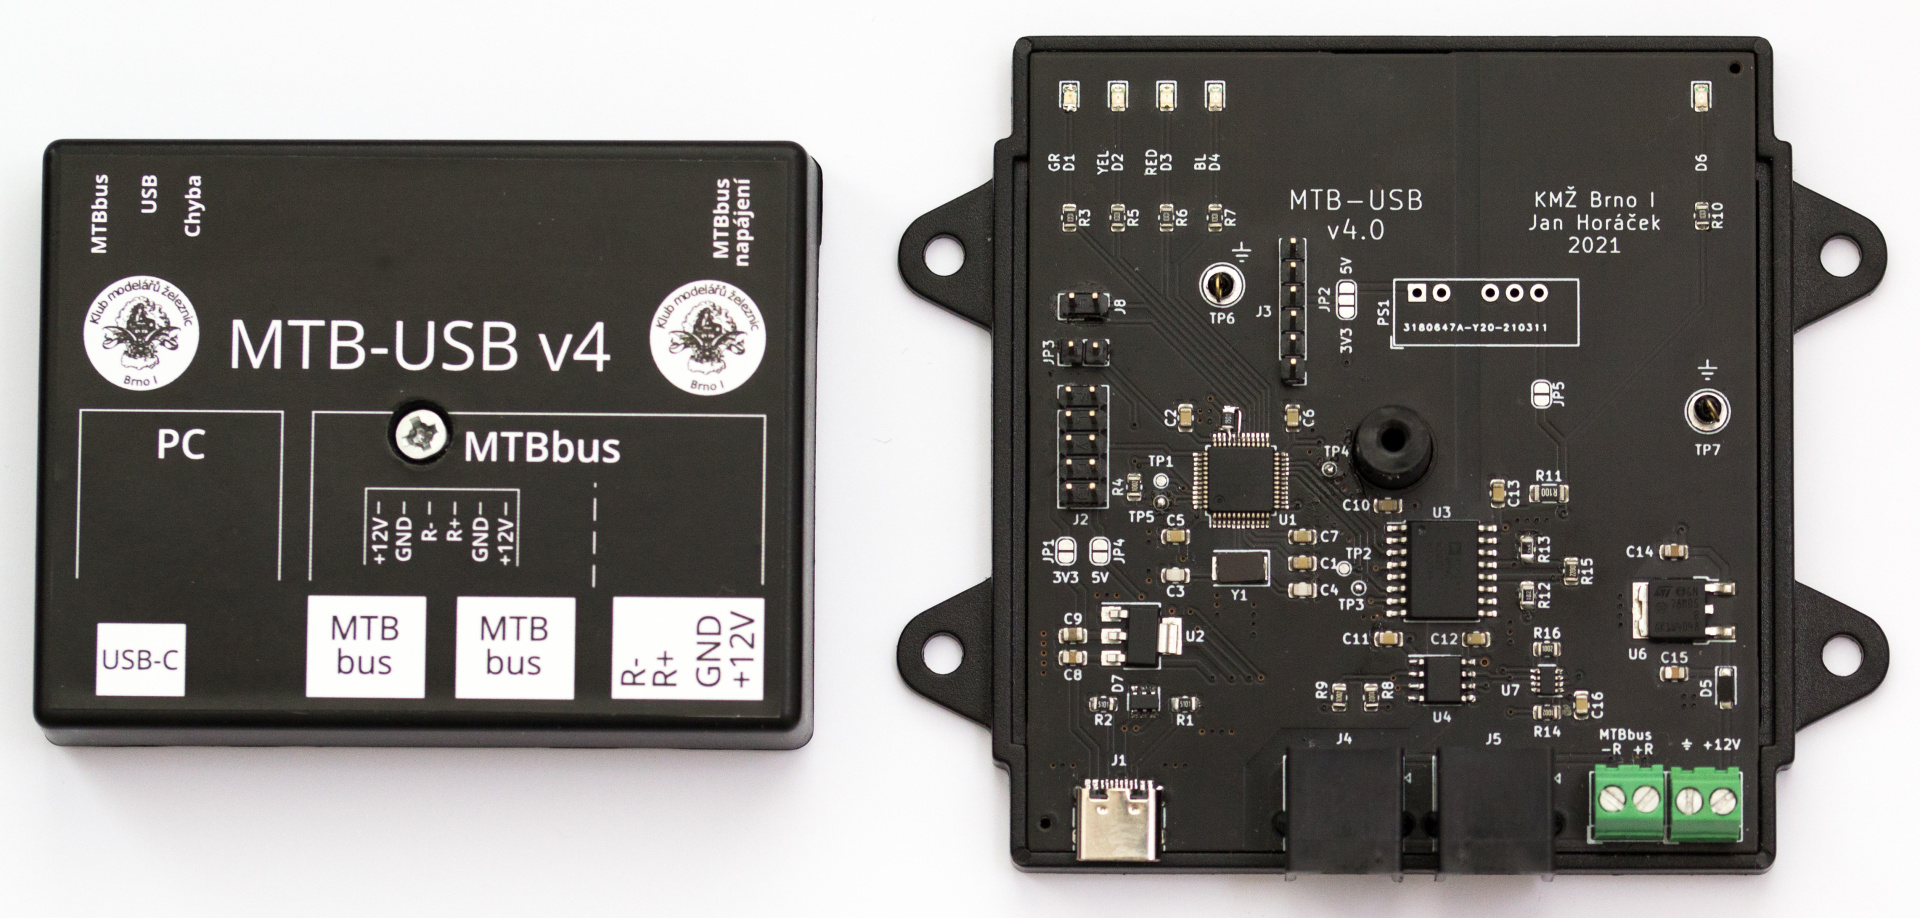
\includegraphics[width=\textwidth]{data/usb-inside.jpg}
\caption{Krabička a deska plošných spojů \gls{mtbusb}.}
\label{fig:mtbusb-prototype}
\end{figure}

Srdcem desky je procesor \texttt{STM21F103}. Jedná se o moderní mikrokontrolér
rodiny \textit{ARM}, který autor zvolil z několika důvodů.

\begin{compactenum}
\item Procesor \texttt{STM32F103} má hardwarovou podporu \gls{usb}.
\item Procesory \texttt{STM32} nabízí velké velikosti pamětí a výpočetní výkon.
\item Procesory \texttt{STM32} se stávají standardy ve vestavěných systémech.
\item Procesory \texttt{STM32} se dají velice snadno debugovat.
\item Procesor \texttt{STM32F103} je jako jeden z mála \texttt{STM} součástí
	\textit{basic} součástek na \url{https://jlcpcb.com/}.
\item Autor se chtěl naučit pracovat s novou architekturou procesorů.
\end{compactenum}

Zastavme se krátce u některých bodů.

Hardwarová podpora \gls{usb} umožňuje výrazně vyšší flexibilitu komunikace
práce s počítačem, než použití historicky zaužívaných převodních obvodů mezi
\gls{usb} a sériovou linkou procesoru. V programu procesoru je tak například
možné definovat, že procesor má více \gls{cdc} linek – druhá se hodí například
pro ladění programu. Procesor může používat libovolnou třídu \gls{usb}. Celé
řešení se tak stává mnohem lépe upravitelné pouze změnou softwaru, což je
zásadně méně pracné, než změna hardwaru.

Všechny desky plošných spojů navrhnuté v rámci této práce, jsou navrženy tak,
aby se daly automaticky osazovat na \url{https://jlcpcb.com/}\footnote{Aktuálně
lze osazovat pouze jednu stranu desky a pouze \textit{SMD} součástky.}. Tato
firma nabízí velice levné automatické osazování malých sérií desek, což výrazně
zjednodušuje nasazení nových desek plošných spojů. JLCPCB rozlišuje tzv.
\textit{basic} a \textit{extended} součástky k osazení, přičemž za
\textit{basic} se neplatí režijní poplatek při osazování. \textit{basic}
součástky jsou ty, které se používají skutečně často (typicky diskrétní
součástky – rezistory, kondenzátory apod.) a které se budou vyrábět i za
desítky let.

Schéma a výkres desky plošných spojů byly vytvořeny v nástroji \textit{KiCad},
který autor této práce používal poprvé. Jedním z hlavních přínosů celé této
práce pro něj je, že se naučil pracovat s novými nástroji. Schéma a výkres
desky plošných spojů jsou k dispozici
online\footnote{\url{https://github.com/kmzbrnoI/mtb-usb-4-pcb}}, schéma je
přiloženo jako příloha této práce (\ref{aa}).

Popišme nyní stručné schéma. Na první pohled je schéma rozděleno na 2 části,
které jsou na desce plošných spojů (\textit{\gls{dps}}) galvanicky oddělené –
\gls{usb} část (vlevo) a \gls{mtbbus} část (vpravo). \gls{usb} část obsahuje
procesor a je napájena přímo z \gls{usb}. \gls{mtbbus} část obsahuje rozhraní
sběrnice \gls{mtbbus} a je napájeno buď z externího zdroje (ze stejného jako
zbytek sběrnice \gls{mtbbus}) nebo přes galvanicky oddělený měnič \texttt{PS1}.
Při osazení desky se osazením nebo neosazením součástek zvolí, která varianta
se bude používat.

Hlavním prvkem \gls{usb} části schématu je již zmíněný procesor
\texttt{STM32F03} (vlevo nahoře). K procesoru jsou připojena diagnostická
rozhraní (\texttt{J2}, \texttt{J3}). Celá \gls{usb} část na napájena z \gls{usb}
portu, přičemž je využito moderního konektoru \gls{usb}-C.

Rozhraní \gls{usb} a \gls{mtbbus} části schématu tvoří galvanicky oddělený
driver sběrnice RS485 typu \texttt{ADM2483}. Jedná se o osvědčený driver,
který zvládá proudy sběrnice až do $200~mA$ \cite{adm2483-datasheet} a je tedy
vhodný pro komunikaci s větším počtem \gls{mtb} modulů.

Specialitou \gls{mtbusb} modulu je měřící obvod \texttt{INA219}, který měří
napětí a proud do sběrnicové části obvodu \texttt{ADM2483} a posílá naměřenou
hodnotu do procesoru (skrze galvanické oddělení sběrnice \textit{I2C}). Počítač
je tak schopen detekovat nestandardní chování sběrnice, například zkrat.
\footnote{Pro tento hardware zatím neí podpora v komunikačním protokolu
s~počítačem a ve firmwaru. Hardware je odzkoušený. Podporu je v~plánu doplnit
v~další verzi.}

Při návrhu desky plošných spojů bylo hlavním problémem do jaké krabičky desku
vložit. \gls{mtbusb} modul totiž typicky není pevnou součástí kolejiště, je
umístěn vedle kolejiště u řídicího serveru. Vyvstal tak požadavek modul zavřít
do krabičky, ideálně s možností uchycení na zeď. Po rešerši byla zvolena krabička
firmy \textit{Digikeijs}, jejíž zásadní výhodou je to, že pro vyvedení konektorů
a indikačních LED není třeba do krabičky frézovat. Navíc lze na krabičku velice
elegantně nalepit potisk, který vysvětluje použití jednotlivých konektorů
a~význam LED. Celé řešení je zobrazeno na úvodním obrázku
\ref{fig:mtbusb-prototype}.


\subsection{Firmware}

Firmware je psaný v jazyce C, který byl zvolen především proto, že ve stejném
jazyce je psána základní knihovna pro interakci s periferiemi procesoru
\textit{STM32 HAL} \cite{stm32-hal}, kterou firmware využívá.

Při práci s periferiemi je využito \textit{Direct Memory Access (DMA)}. Pro
komunikaci přes \gls{usb} byla využita komunitní knihovna \texttt{libusb\_stm32},
\footnote{\url{https://github.com/dmitrystu/libusb_stm32}}.

Celý firmware je k dispozici pod opensource licencí na
\url{https://github.com/kmzbrnoI/mtb-usb-4-fw}.

\section{\gls{mtbuni} v4}

Další komponentou nového systému \gls{mtb} je nový modul typu \gls{mtbuni}.
Tento modul vznikl, aby bylo možné provádět nové instalace systému \gls{mtb}
a rozšiřovat současné instalace o~nové moduly.

\subsection{Základní parametry modulu}

\begin{table}[h]
	\begin{tabularx}{\textwidth}{lX}
		\toprule
		Vstupy & 16 digitálních vstupů \\
		Výstupy & 16 výstupů v~režimu otevřeného kolektoru, všechny umožňují
		kmitání a generování \gls{scom} signálu \\
		Napájení & 7–17 V~DC \\
		Adresování & pomocí jumperů \\
		Procesor & ATmega128 \\
		\bottomrule
	\end{tabularx}
	\caption{Základní parametry modulu \gls{mtbuni} v4}
	\label{tab:mtbuni-params}
\end{table}

Aktuální modul \gls{mtbuni} má 16 digitálních vstupů a 16 digitálních výstupů.
Tento počet se autor práce rozhodl zachovat, protože vhodně škáluje pro malé
i~velké stanice. Současné \gls{mtbuni} a MTB-TTL desky používají různé konektory
pro připojení periferií: svorkovnice nebo nasouvací konektory typu \texttt{PSH}
\footnote(Např. \url{https://www.gme.cz/konektor-se-zamkem-psh02-04pg}.).
Modul \gls{mtbuni} v4 umožňuje variantní osazení jak svorkovnic, tak konektorů
\texttt{PSH}. Tím modul slučuje současné moduly \gls{mtbuni} a MTB-TTL do jediné
desky plošných spojů, což zjednodušuje údržbu a vývoj.

Hardwarové řešení výstupů je ponecháno: výstupy jsou v~režimu otevřených
kolektorů. Výstupy jsou řízení skrze obvody \texttt{ULN2803}, které umožňují
dostatečný výstupní proud až 0.5~A~/~8 výstupů. Všechny výstupy umožní kmitání
i zasílání signálu \gls{scom} \ref{scom}.

Modul obsahuje 16 digitálních vstupů. Podporu IR čidel bude řešit samostatná
deska, viz \ref{}.

Deska plošných spojů je navrhnuta tak, aby byly zachovány rozměry a umístění
upevňovacích otvorů se současným nejmenším modulem – MTB-TTL.

Návrh této desky vznikal ve spolupráci s~\textit{Mendelovou univerzitou v~Brně},
schéma vytvořil Robert Čížek, deska plošných spojů, firmware a koncepční návrh
modulu je dílem autora této práce.


\subsection{Hardware}

Při návrhu modulu připadaly v~úvahu dva zásadní přístupy:

\begin{compactenum}
\item malý proces, posuvné registry na vstupy a výstupy;
\item velký procesor, vstupy a výstupy připojené přímo na piny procesoru.
\end{compactenum}

Autor této práce zvolil přístup (2), protože chtěl minimalizovat počet
součástek na desce a protože v~dnešní době není problém sehnat fyzicky malý
procesor s~40 piny.

Schéma i deska plošných spojů jsou openhardware projekt, dostupné na
\url{https://github.com/kmzbrnoI/mtb-uni-4-ele}, schéma také v~příloze
\ref{}. Zmiňme nyní zajímavé prvky schématu a desky plošných spojů.

Jádrem desky je procesor \texttt{ATmega128A}. Autor této práce si zvolil
procesor architektury \textit{AVR}, protože s~používáním těchto procesorů má
dlouholeté zkušenosti. Model \textit{ATmge128a} byl pak zvolen proto, že je to
nejmenší model rodiny \textit{ATmega}, který obsahuje požadované množství pinů.

\subsubsection{Vstupy}

Nový \gls{mtbuni} v4 modul oproti modulu současnému obsahuje řádnou ochranu
vstupů. Ochranný obvod vstupů vznikl ve spolupráci Jana Horáčka, Michala
Petrilaka a Roberta Čížka. Zapojení jednoho vstupu je demonstrováno na obrázku
\ref{fig:mtbuni-input}.

\begin{figure}[ht]
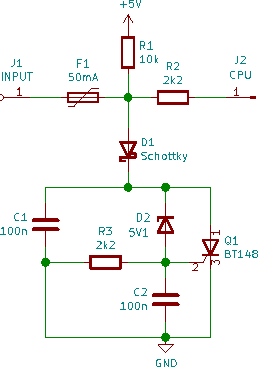
\includegraphics[width=0.4\textwidth]{data/uni-input/uni-input.pdf}
\caption{Zapojení vstupu modulu MTB-UNI.}
\label{fig:mtbuni-input}
\end{figure}

Schéma \ref{fig:mtbuni-input} je rozděleno na 2 části schottkyho diodou
\texttt{D1}. Horní část včetně diody \texttt{D1} je pro každý z~16 vstupních
pinů zvlášť, spodní je vždy pro osmici pinů společná.

Očekává se, že periferie připojená k~pinu (\texttt{INPUT}) bude tento pin
uzemňovat, případně že bude pin v~režimu \gls{ttl}. Každý vstup obsahuje
pull-up rezistor \texttt{R1}, aby měl vstupní signál vždy definovanou napěťovou
úroveň. Pull-up rezistor je relativně tvrdý, aby se zabránilo ovlivňování
vstupů okolním rušením, které signál \gls{dcc} při přenášení větších proudů
bohužel generuje.

K~procesoru vede signál přes ochrannou pojistku \texttt{F1} (význam vysvětlíme
niže) a ochranný rezistor \texttt{R2}. Tento rezistor zabraňuje naproudu do pinu
procesoru a tím jeho zničení.

Funkcí celého obvodu od \texttt{D1} níže je vyzkratovat vstup na zem v~momentě,
kdy je na něj přivedené vyšší než dovolené napětí. Pin procesoru povoluje
napětí nejvýše $5.5~V$ \cite{atmega128-datasheet}. Jakmile se vstupní napětí
začne blížit $5.4~V$ ($5.1~V$ zenerova dioda \texttt{D2} + $0.3~V$ schottkyho
dioda \texttt{D1}), začne se dioda \texttt{D2} otevírat a tím se začne otevírat
i tyristor \texttt{Q1}.\footnote{V praxi tato situace nastává už při trochu
nižším napětí, cca $5.3~V$, protože pro otevření \texttt{Q1} stačí, aby se
\texttt{D2} otevřela jen nepatrně.} Vstupní proud proteče přes \texttt{Q1} do
země a tím je vstup zkratován (do země). Proud je limitován pojistkou \texttt{F1}.
Tyristor \texttt{Q1} dimenzován jako výkonový, protože do něj může téct zkratový
proud všemi 8 piny, navíc chování polymerové pojistky umožňuje krátkodobé řádově
větší proudy, které musí tyristor zvládnout \cite{polyfuse-behavior}.

V~praxi se často používá zapojení \textit{vstup – ochranný rezistor – pull-up –
pin procesoru}. V~zapojení \gls{mtbuni} desky za oproti tomu používá zapojení
\textit{vstup – pull-up – ochranný rezistor – pin procesoru}. Výhodou zapojení,
které bylo implementováno do \gls{mtbuni} modulu, je, že na vstupu procesoru
není napěťový dělič. V~případě, že vstup má například napětí $0.7~V$ (což se
snadno stane například tehdy, když periferie používá výstupy typu otevřené
kolektory), je toto napětí přivedeno přímo na pin procesoru a tedy spolehlivě
detekováno jako logická nula\footnote{V~\gls{mtbuni} desce je detekováno
jako logická jednička, protože modul používá inverzní logiku.}. Při zapojení
prvního typu by na pinu procesoru vznikl napěťový dělič, který by mohl ohrozit
spolehlivost čtení pinu.

\subsubsection{Výstupy}

Na výstupech je použito již zmiňovaných obvodů \texttt{ULN2803}. Za obvody
je vřazena polymerová pojistka. Protože obvod \texttt{ULN2803} specifikuje
proudové omezení $0.5~A$ / všechny výstupy \cite{uln2803-datasheet}, nemohou
samostatné pojistky zajistit nepřetížení modulu a zároveň umožnit využití
maximálního proudu. Proto jsou na desce plošných spojů \gls{mtbuni} v4 obvody
\texttt{ULN2803} jako jedny z~mála osazeny v~paticích v~\textit{DIL} provedení.

Výstupy obsahují ochranu proti přivedení vysokého napětí, kterou realizuje
stejný obvod, jako na obrázku \ref{fig:mtbuni-input} (obvod pod diodou
\texttt{D1}). Obdobný obvod realizuje ochranu také proti vysokému napájecímu
napětí celého modulu. Viz kompletní schéma \ref{mtbuni-sch}.

\subsubsection{Adresování}

Adresa modulu \gls{mtbuni} v4 je určena jumpery na modulu. Při návrhu modulu
vyvstala diskuze, jaký je nejlepší způsob adresování modulů, přičemž soupeřily
přístupy

\begin{compactenum}
\item modul má adresu uloženou v~EEPROM, adresu je možné změnit přes \gls{mtbbus}
\item adresa se konfiguruje přímo jumpery na modulu.
\end{compactenum}

Druhý přístup, který zvolil autor této práce, si vysloužil mnohou kritiku.
Autor si však stojí za tím, že snadná a především vždy pravdivá identifikace
adresy modulu prostým pohledem na něj stojí za 8 vstupních pinů procesoru navíc.

Pro elegantní řešení přístupu (1) je třeba mít na desce tlačítko. Tlačítko se
na desce nachází, takže pokud by byla v~budoucnu snaha přejít na přístup (1),
je změna otázkou změny firmwaru.

\subsection{Deska plošných spojů}

Deska plošných spojů je navrhnuta tak, aby byly zachovány rozměry a umístění
upevňovacích otvorů se současným nejmenším modulem – MTB-TTL. Deska je dvouvrstvá
(protože to stačí), používají se primárně SMD součástky velikosti 0805 umístěné
na spodní stranu desky (aby šla \gls{dps} automaticky osazovat). Na obrázku
\ref{dig:mtb-uni-v4} je prototyp desky \gls{mtbuni} v4.0. Poslední verze je
verze 4.2, která oproti 4.0 obsahuje více \textit{SMD} součástek a opravuje
některé chyby prototypu.

\begin{figure}[ht]
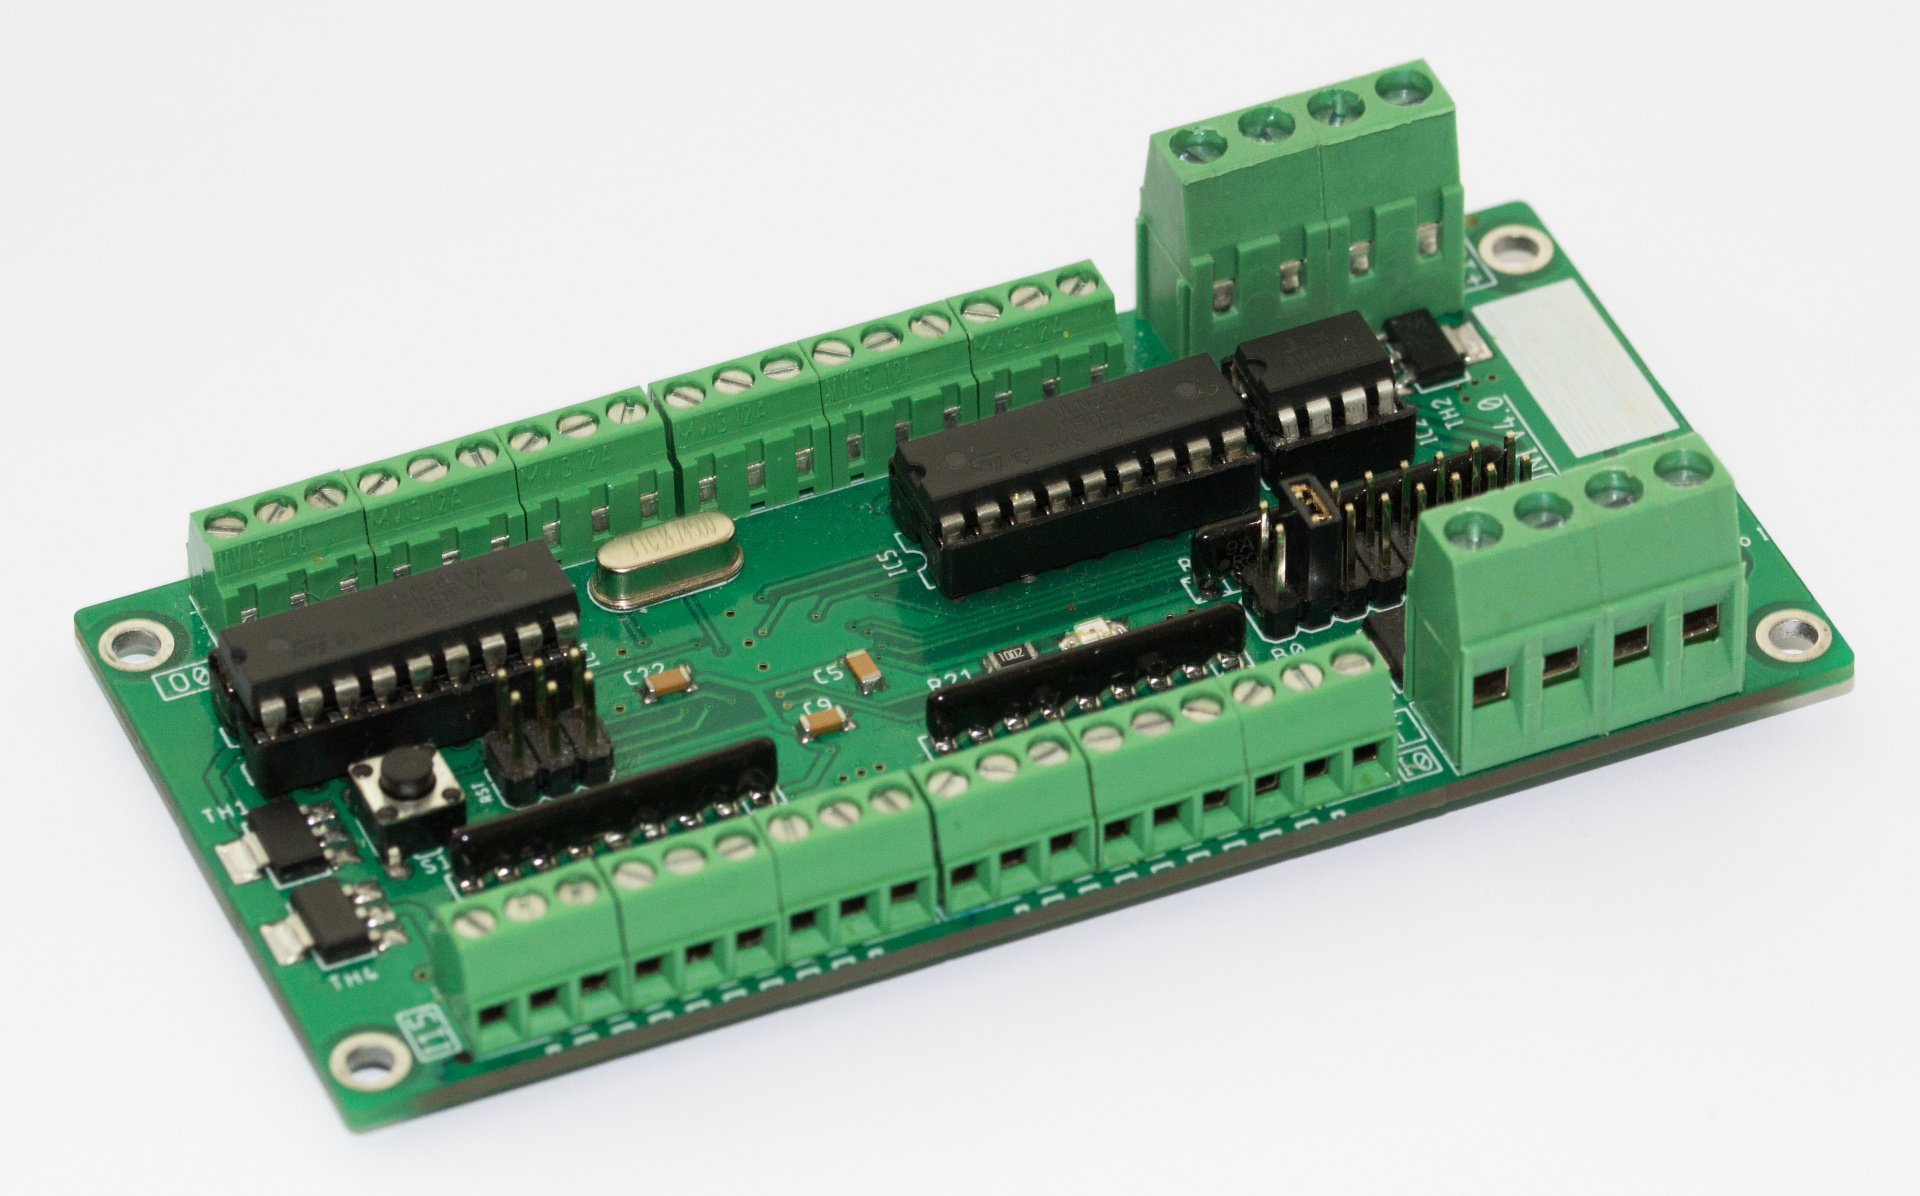
\includegraphics[width=0.9\textwidth]{data/uni-v40-screw-all.jpg}
\caption{\gls{mtbuni} v4.0.}
\label{fig:mtb-uni-v4}
\end{figure}

\subsection{Firmware}

Firmware pro procesor \textit{ATmega128A} je psán v~jazyce C a je dostupný
pod opensource licencí na \url{https://github.com/kmzbrnoI/mtb-uni-4-fw}.

Zajímavým prvkem firmwaru je podpora jeho aktualizace přímo přes sběrnici
\gls{mtbbus}. Firmware obsahuje 2 části:

\begin{compactenum}
\item hlavní program,
\item bootloader
\end{compactenum}

Bootloader je nahraný ve speciální části paměti (na konci) a zajišťuje
aktualizaci hlavního programu. Bootloader je měnitelný pouze přímým
programování procesoru, nikoliv přes \gls{mtbbus}. Firmware tak v~zásadě
obsahuje 2 samostatné programy, které se po zkompilování slinkují dohromady.

Bootloader umí pouze aktualizovat firmware a kontrolovat jeho konzistenci.
Kontrola konzistence firmwaru je implementována pomocí uložení \textit{CRC-16}
kontrolního součtu a počtu aktivních stránek paměti na konkrétních adresách
paměti (na konci těsně před bootloaderem).

\section{MTB-2-AVR} \label{sec:mtb-2-avr}

Aby nebylo nutné všechny současné \gls{mtbuni} desky vyměňovat za desky nové,
je třeba staré desky povýšit tak, aby podporovaly nový protokol \gls{mtbuni} v4.
Díky omezenosti procesoru v~současných modulech \gls{mtbuni} není možné tuto
úpravu provést pouze změnou firmwaru, viz \ref{prev}.

Výhodou je, že procesory na současných \gls{mtbuni} modulech jsou
v~\textit{DIL} patici. Nabízí se tedy přirozená cesta najít nový procesor
odpovídajícího rozložení pinů. Procesor, který by měl vyhovující rozložení pinů
a požadované parametry bohužel neexistuje. Uvažován byl například procesor
TODO. Proto se autor této práce vydal cestou výroby nástavné desky, která se
zasune do \textit{DIL} patice současné \gls{mtbuni} desky a na sobě bude mít
\textit{smd} procesor.  Správné napojení pinů se vyřeší na nástavné desce
plošných spojů.

Tuto myšlenku implementuje deska \textit{MTB-2-AVR}, viz obrázek
\ref{fig:mtb-2-avr-alone}.

\begin{figure}[ht]
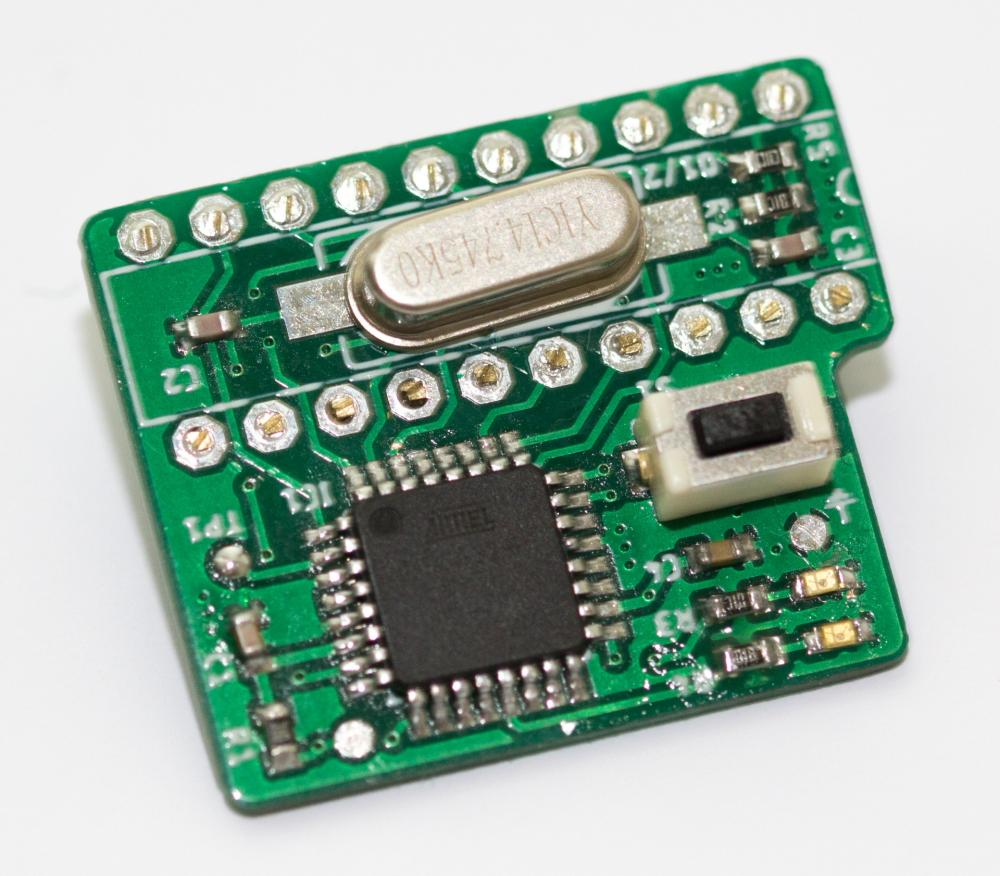
\includegraphics[width=0.4\textwidth]{data/uni-2-upgrade-alone.jpg}
\caption{Nástavná deska \textit{MTB-2-AVR}.}
\label{fig:mtb-2-avr-alone}
\end{figure}

\begin{figure}[ht]
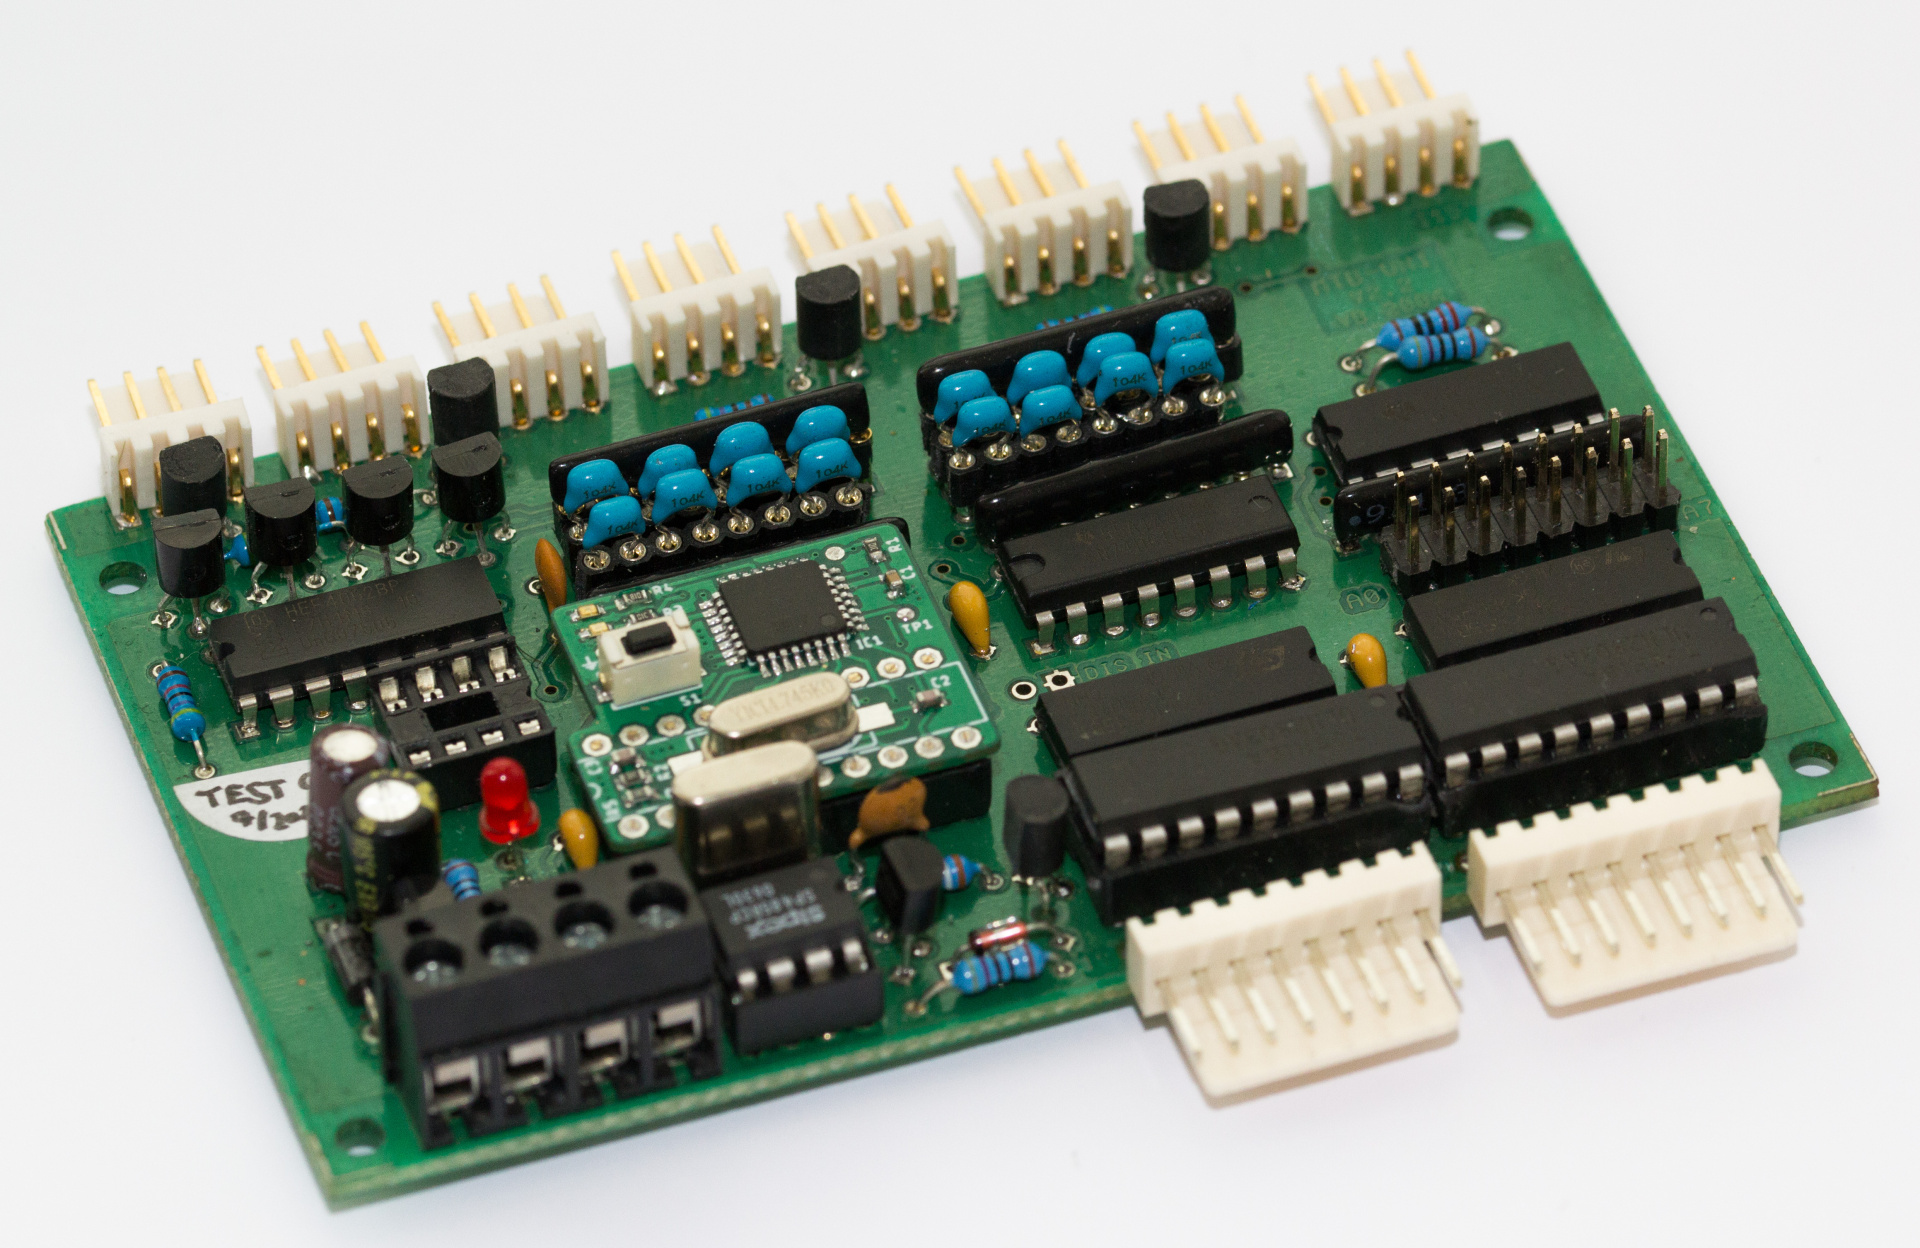
\includegraphics[width=0.9\textwidth]{data/uni-2-upgrade-all.jpg}
\caption{Nástavná deska \textit{MTB-2-AVR} v~modulu \gls{mtbuni} v2.}
\label{fig:mtb-2-avr-inside}
\end{figure}

Deska je navržena tak, aby se dala umístit místo procesoru libovolného z~modulů
\gls{mtbuni}, \textit{MTB-UNIm} a \textit{MTB-TTL}. Srdcem desky je procesor
\textit{ATmega328p} autorovy oblíbené architektury procesorů \textit{AVR}.
Konkrétně tento model byl zvolen, protože obsahuje dostatečnou kapacitu paměti
na bootloader a protože jej \textit{Jlcpcb} má mezi \textit{basic součástkami}
(viz \ref{todo}).

Schéma a deska plošných spojů jsou vyvinuty jako openhardware projekt a dostupné
na \url{https://github.com/kmzbrnoI/mtb-2-avr-pcb}. Deska plošných spojů obsahuje
kromě procesoru chybějící LED, aby každá \gls{mtb} deska měla zelenou, žlutou a
červenou LED. Dále obsahuje krystal, protože původní krystal na \gls{mtbuni}
desce je mimo rozsah dovolených hodnot kmitočtů krystalu pro procesor
\textit{ATmega328p}. Deska dále obsahuje tlačítko (pro unifikaci hardwaru
s~\gls{mtbuni} v4 modulem).

Jak již bylo zmíněno, tato nástavá deska se bude osazovat do patic současných
\gls{mtbuni} i \textit{MTB-TTL} desek. Přitom u~\gls{mtbuni} desek by měl procesor
podporovat IR čidla na vstupech. Procesor proto detekuje v~jaké desce se nachází
(byl identifikován a využit HW rozdíl různých typů desek) a podle toho buď
zapne nebo vypne podporu IR čidel. Do počítače pak přes \gls{mtbbus} protokol
nahlásí, jestli IR čidla podporuje nebo ne.

Zde mimochodem využijeme \textit{Module specific command} (\ref{subsub:mtbbus-messages}). Modulu
\textit{MTB-2-AVR} lze poslat příkaz, aby znovu provedl autodetekci typu
desky, do které je vložené, případně nastavit typ desky ručně.

Firmware je pod opensource licencí dostupný na
\url{https://github.com/kmzbrnoI/mtb-2-avr-fw}. Firmware se opět skládá
z~bootloaderu a hlavního programu.

\section{IRdet} \label{sec:irdet}

V~rámci této práce a ve spolupráci s~\textit{Laboratoří řízení kolejových
vozidel MENDELU} vznikla jednoduchá deska, která umožňuje připojení až 8 IR
čidel (viz \ref{ir}). Deska hlásí stav IR čidel pomocí opticky oddělených
8~digitálních výstupů. Výstupy desky lze připojit na vstupy \gls{mtbuni}
modulu, nebo například k~signalizačním diodám do pultu řízení obsluhy.
Deska \textit{IRdet} není nijak závislá na systému \gls{mtb}. V~této práci ji
však uvádíme, protože vznikla především proto, aby bylo možné plnohodnotně
nahradit současné \gls{mtbuni} moduly (s~přímou podporou IR čidel) použitím
nových modulů \gls{mtbuni} v4 a desek \textit{IRdet}.

\begin{table}[h]
	\begin{tabularx}{\textwidth}{lX}
		\toprule
		Vstupy & Až 8 IR čidel \\
		Výstupy & 8 digitálních opticky oddělených výstupů \\
		Napájení & 10–17 V~DC \\
		Proud IR diodami & nastavitelný osazením příslušného rezistoru \\
		\bottomrule
	\end{tabularx}
	\caption{Základní parametry desky \textit{IRdet}}
	\label{tab:mtbuni-params}
\end{table}

Schéma zapojení a deska plošných spojů jsou k~dispozici jako openhardware
projekt na \url{https://github.com/kmzbrnoI/irdet-ele}, firmware je psán jako
opensource projekt a je dispozici na
\url{https://github.com/kmzbrnoI/irdet-fw}.

Hlavní komponentou návrhu je procesor řady \textit{Atmega8*}. Lze osadit
libovolný z~procesorů \textit{ATmega8a}, \textit{ATmega88}, \textit{ATmega328}
a kompatibilní. Vstupy od fototranzistorů jsou zapojeny v~režimu kapacitní
vazby, viz \ref{cap-link}. Vysílací IR diody jsou buzeny přes tranzistory.
Proud do vysílacích diod je řízen omezovacím rezistorem na stabilizovaném
napětí.

Deska je tradičně navrhnuta především z~\textit{SMD} součástek (velikosti 0805)
jako dvoustranná s~cílem osazovat součástky automaticky. Napájení se očekává
ze stejného rozvodu jako je napájecí rozvod \gls{mtb} desek (ačkoliv to díky
optickému oddělení vstupů není nutné).

\begin{figure}[ht]
\subfigure{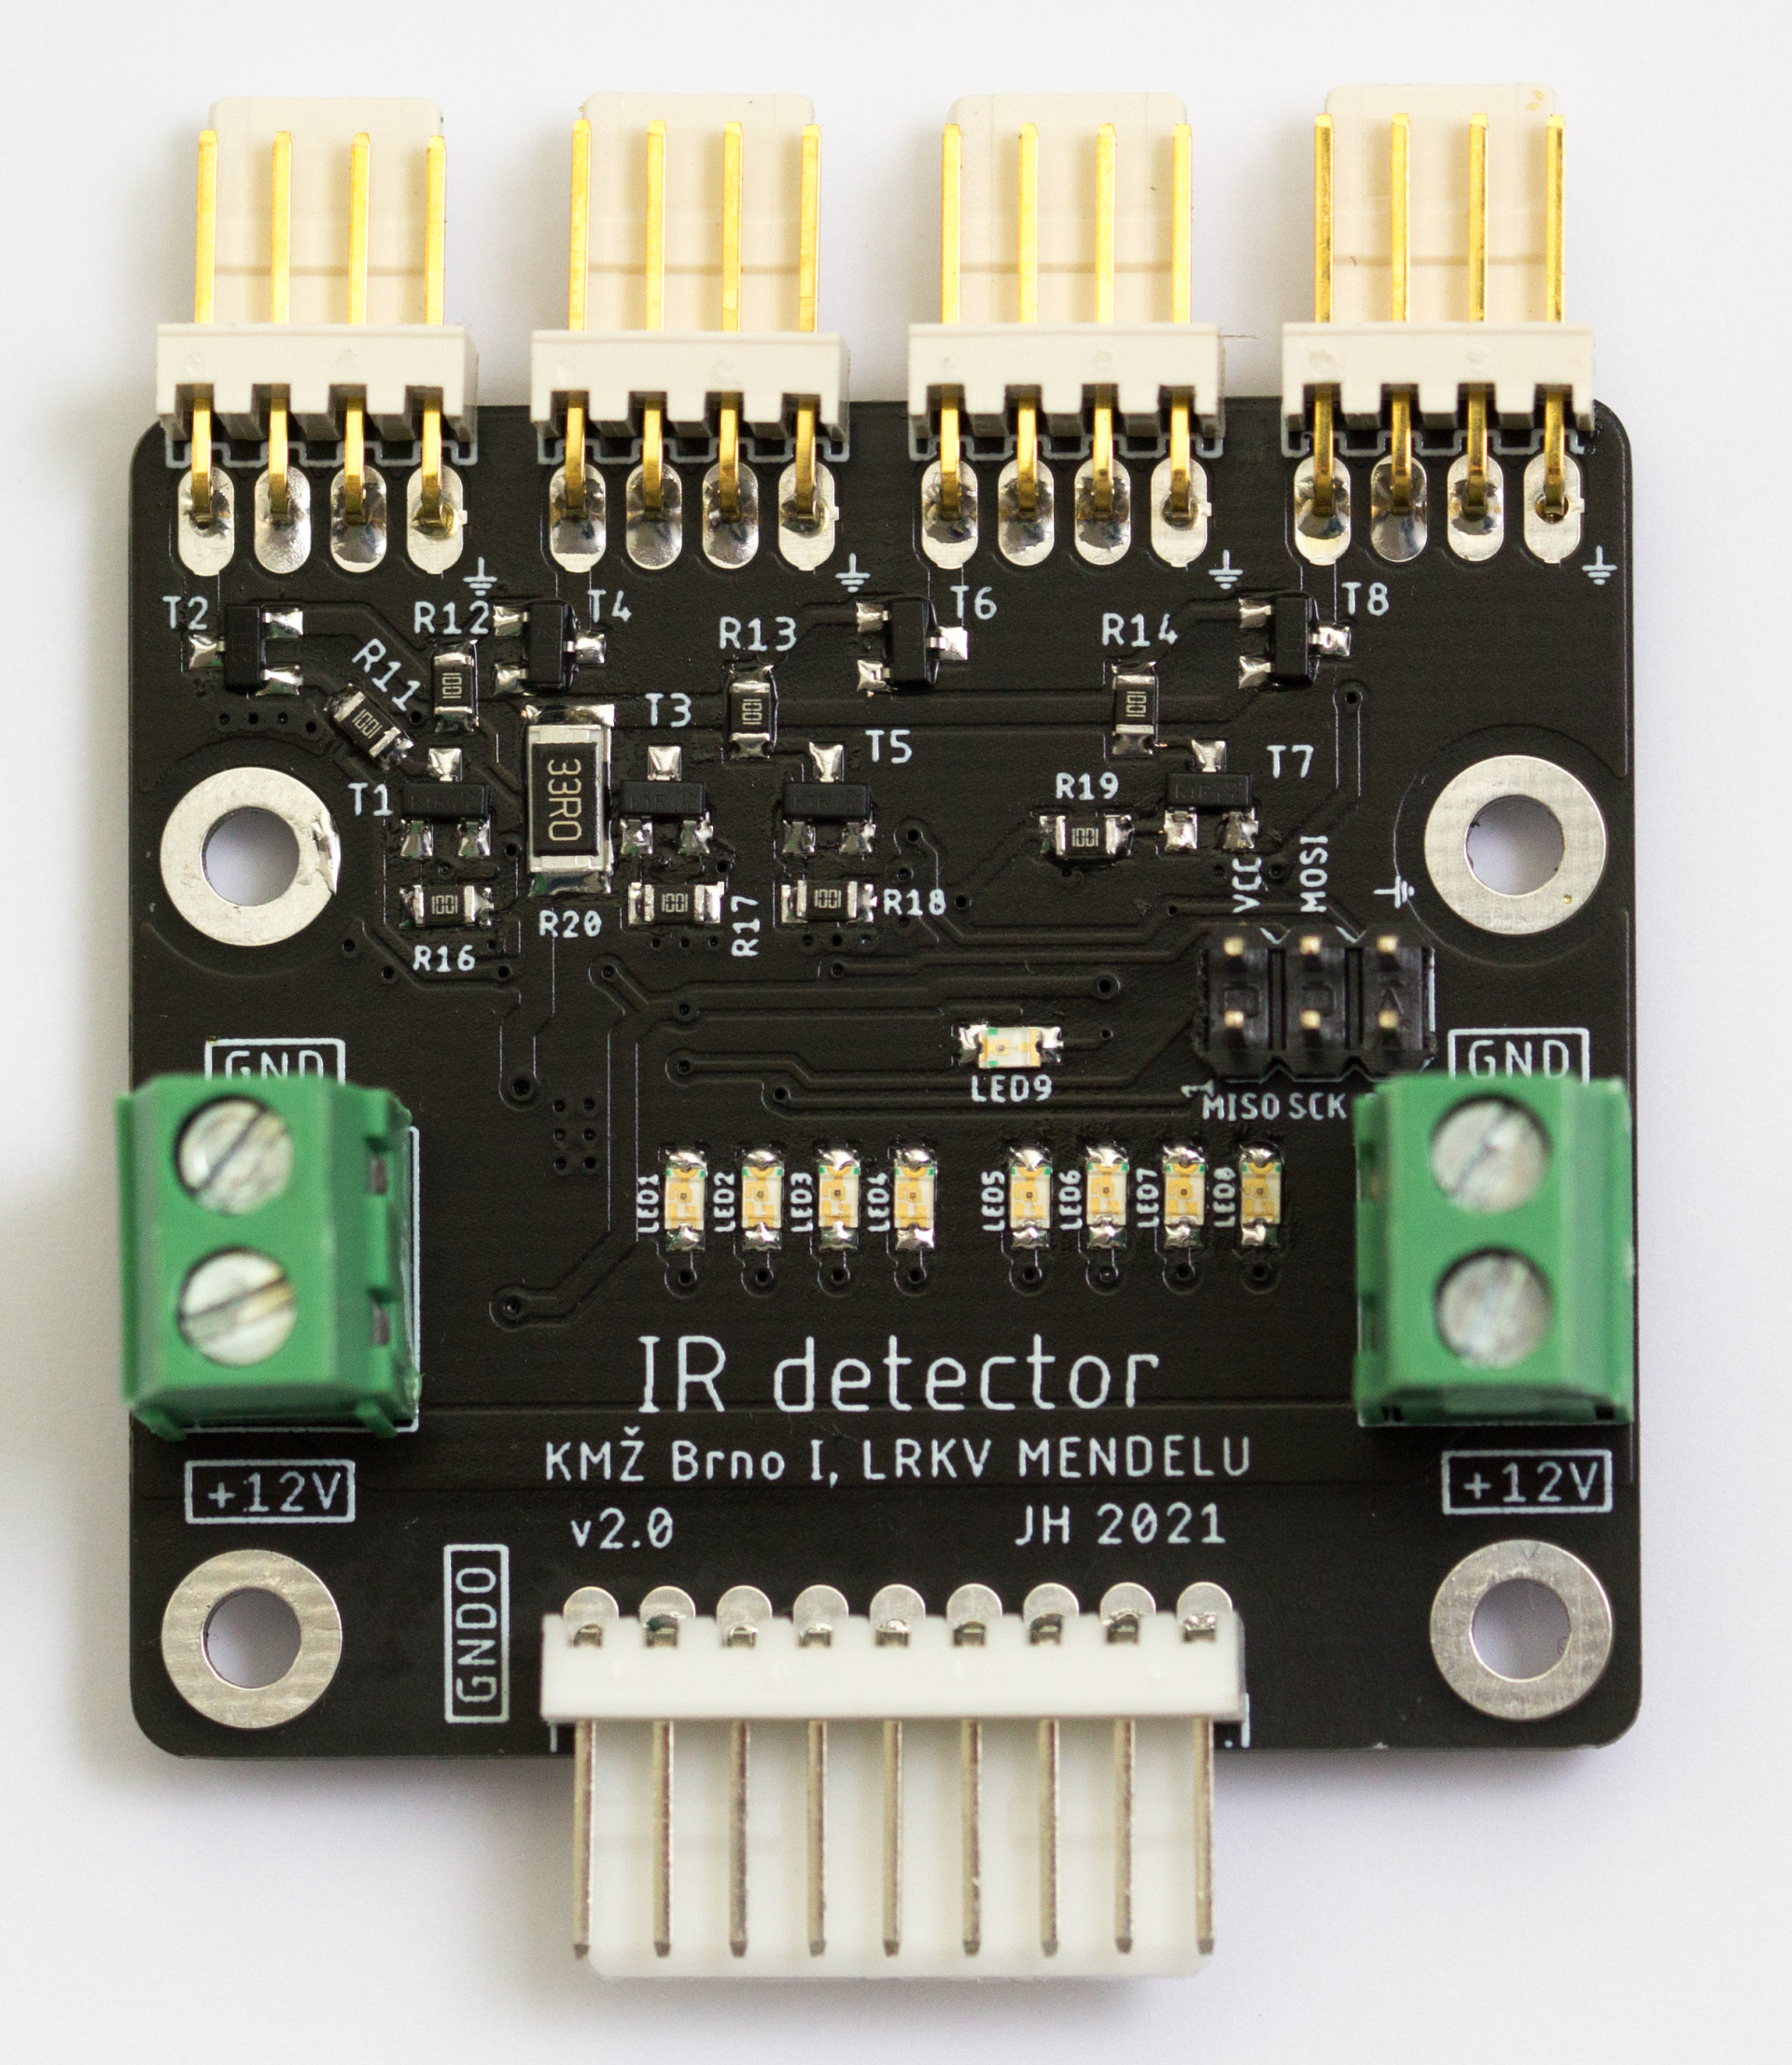
\includegraphics[width=0.5\textwidth]{data/irdet-front.jpg}}
\caption{Produkční verze desky IRdet}
\label{fig:irdet}
\end{figure}

\newpage
\section{MTB Daemon}

\textit{\gls{mtb} Daemon} je první ze dvou počítačových aplikací, která v~rámci
této práce vznikla. Jejím hlavním úkolem je připojit se k~\gls{mtbusb} modulu a
umožnit jeho ovládání více různým aplikacím. K~tomuto účelu vystavuje \gls{mtb}
Daemon \gls{tcp} server, ke kterému se řídicí programy mohou připojit.

\subsection{Protokol TCP serveru} \label{sec:daemon:proto}

\gls{tcp} server musí umožňovat oboustrannou komunikaci – jak od klienta k~serveru
(\textit{požadavek, odpověď}), tak od serveru ke klientovi (\textit{asynchronní
události}). Například protokol \textit{http} v~kombinaci s~\textit{REST \gls{api}}
tedy není vhodné použít. Z~běžně používaných technologií byly zvažovány
\textit{websockets}, ty ale kvůli složitější inicializaci nebyly využity.

Autor zvolil snad nejjednodušší možný komunikační protokol: \gls{tcp} spojení
je udržováno trvale otevřené, posílají se textová data, každý řádek je jedna
zpráva. Textová data jsou ve formátu \textit{json}.

Textový protokol byl zvolen, aby bylo možné data číst lidským okem
(snadná diagnostika). Očekává se, že řídicí aplikace se bude připojovat
převážně ze stejného počítače, na kterém běží \gls{mtb} Daemon, nemá tedy smysl
šetřit \uv{kapacitu linky} binárním protokolem.
Formát \textit{json} byl zvolen proto, že je dnes moderním standardem pro
výměnu dat mezi aplikacemi. Snad všechny majoritní programovací jazyky obsahují
ve svých standardních knihovnách podporu pro práci s~\textit{json}.

Zprávy se posílají v~kódování \textit{UTF-8}. Nyní uvedeme příklad
dvou zpráv (pro přehlednost je každá zpráva rozdělena na více řádků, ve
skutečnosti se posílá na jednom řádku):

\begin{verbatim}
{
    "command": "mtbusb",
    "type": "request",
    "id": 42
}
\end{verbatim}
\newpage
\begin{verbatim}
{
    "command": "mtbusb",
    "type": "response",
    "id": 42,
    "status": "ok",
    "mtbusb": {
        "connected": true,
        "type": 1,
        "speed": 115200,
        "firmware_version": "1.0",
        "protocol_version": "1.0",
        "active_modules": [1, 5, 2, 121]
    }
}
\end{verbatim}

Zprávy jsou tří typů (\texttt{type}):

\begin{compactenum}
\item \texttt{request} (zpráva od klienta serveru),
\item \texttt{response} (odpověď na \texttt{request}),
\item \texttt{event} (asynchronní událost – od serveru klientovi).
\end{compactenum}

Aby klient věděl, která odpověď patří kterému požadavku (klient může posílat
více požadavků rychle za sebou), lze u~každého požadavku uvést \texttt{id}
(číslo). Příslušná odpověď pak obsahuje stejné \texttt{id}.

Klient se může zaregistrovat ke konkrétním modulům příkazem \\
\texttt{module\_subscribe} (a odregistrovat příkazem
\texttt{module\_unsubscribe}). Pokud je klient zaregistrovaný k~nějakému modulu,
chodí mu asynchronní události o~změně stavu modulu (např. změna stavu vstupu).
Klienti si tak mohou volit, o~data kterých \gls{mtb} modulů mají zájem.

Kompletní specifikace protokolu je k~dispozici
online\footnote{\url{https://github.com/kmzbrnoI/mtb-daemon/tree/master/tcp-protocol}}.

\subsection{Volba nástrojů} \label{sec:daemon:tools}

\gls{mtb} Daemon je klíčová aplikace infrastruktury řízení kolejiště. Proto se
autor rozhodl ji programovat v~programovacím jazyce se silným statickým typovým
systémem.

Jako programovací jazyk bylo zvoleno \texttt{C++} (\texttt{C++17})
s~frameworkem \texttt{Qt}, který nabízí přímočaré knihovny pro komunikaci se
sériovým portem a pro síťovou komunikaci. U~knihoven zejména není třeba
složitěji řešit vlákna. \texttt{C++} a \texttt{Qt} umožňují multiplatformní
řešení aplikace – \gls{mtb} Daemon lze zkompilovat a spustit jak na
OS Linux, tak OS Windows.

\subsection{Implementace} \label{sec:daemon:impl}

Aplikace \gls{mtb} Daemon je psána jako jednovláknová konzolová aplikace.
Při návrhu byla zvažována i~možnost implementovat aplikaci jako okenní
(operátor obsluhy by přes aplikaci konfiguroval \gls{mtb} moduly a~měl by
přehled o~stavu sběrnice), nakonec však byl zvolen přístup, kdy aplikace pouze
vystavuje \gls{api}. Konfigurace se načítá ze souboru. V~případě zájmu o~vytvoření
grafického nástroje pro interakci se systémem \gls{mtb} bude tento systém
vytvořen jako další z~klientů aplikace \gls{mtb} Daemon nebo jako
nástroj pro přímou úpravu konfiguračního souboru.

Při implementaci bylo třeba vyřešit, jak zaručit, aby sběrnici nemohli ovládat
neautorizovaní klienti. V~současnosti je implementován pouze velice hrubý
autorizační mechanismus – server poslouchá na specifických rozhraních,
typicky jenom \textit{localhost}. Očekává se, že lokální stroj je server
kolejiště, na kterém by měly běžet výhradně bezpečné aplikace. V~budoucnu možná
autor přistoupí k~implementaci autentizace založené na povolení konkrétních
IP adres klientů. Očekává se, že klienti aplikace \gls{mtb} Daemon jsou trvale
připojená, nemigrující síťová zařízení, která řídí nějaký konkrétní systém
kolejiště, proto není nutné implementovat žádný složitější autentizační
mechanismus.

Jednotliví klienti mohou ovládat libovolné výstupy libovolných \gls{mtb}
modulů.  Při návrhu aplikace vyvstala otázka, zda by v~konfiguraci nemělo být
specifikováno, který klient může ovládat který výstup (kterého modulu). Po
uvážení však bylo od tohoto nápadu upuštěno, protože by vyžadoval netriviální
(ručně psanou) konfiguraci navíc a identifikaci klientů. Očekává se, že klienti
připojující se k~\gls{mtb} Daemon jsou buď autonomní aplikace, nebo
aplikace, které řízení přístupu svých uživatelů implementují na své vlastní
úrovni. Pokud by nastala problematická situace, kdy dva klienti chtějí ovládat
stejný výstup, jedná se o~chybu v~klientské aplikaci nebo její konfiguraci,
nikoliv o~nekalý záměr, kterému by měl systém vší silou zabránit. \gls{mtb}
Daemon nastavení jednoho výstupu více klienty umožní, ale současně zaloguje
varování. To umožňuje operátorovi takovou situaci rozpoznat a konfiguraci
klientských aplikací opravit.

\gls{mtb} Daemon si pamatuje, který klient nastavil který výstup a při
odpojení klienta provede reset jím nastavených výstupů do základního stavu.

Aplikace obsahuje hierarchii tříd (ve vztahu dědičnosti) reprezentujících
jednotlivé typy \gls{mtb} modulů. \gls{tcp} protokol také počítá s~různými typy
modulů. Aplikace je tak připravena na přidání budoucích nových typů \gls{mtb}
modulů.

MTB Daemon je pod opensource licencí dostupný
online\footnote{\url{https://github.com/kmzbrnoI/mtb-daemon}}.

\newpage
\section{hJOP MTB Network RCS knihovna} \label{sec:mtb-net-lib}

Knihovna \textit{hJOP MTB Network RCS library} je posledním softwarem implementovaným
v~rámci této diplomové práce. Jeho účelem je propojit stávající systém řízení
kolejiště \textit{hJOP}\footnote{\url{https://hjop.kmz-brno.cz/}, používá se
pro řízení všech kolejišť v~\gls{kmz}. Implementovaný na platformě OS Windows.}
a~\textit{MTB daemon}. \textit{hJOP} pro přístup k~hardwaru řízení
příslušenství používá tzv. \textit{RCS API} \footnote{\textit{Railroad Control
System API}, viz \url{https://hjop.kmz-brno.cz/rcs}.}. Systém pro řízení
příslušenství se připojuje k~\textit{hJOP} jako dynamicky linkovaná knihovna,
která implementuje \textit{RCS API}.

Byla tedy implementována jednoduchá knihovna, která se přilinkuje do
\textit{hJOP} a připojí se k~\textit{MTB daemon}. Pro implementaci bylo
opět zvoleno \texttt{C++} a framework \texttt{Qt}. K~této volbě vedly důvody
popsané v~kapitole \ref{sec:daemon:tools}.

Na samotné implementaci knihovny toho není mnoho zajímavého, proto ji uvádíme
jen stručně. Knihovna je pod opensource licencí dostupná
online\footnote{\url{https://github.com/kmzbrnoI/mtb-net-lib}}.


\chapter{Závěr} \label{chap:zaver}
Tato diplomová práce demonstrovala, že pro vytvoření plnohodnotného \gls{plc}
systému je třeba zvládnout širokou škálu dílčích kroků. Od návrhu komunikačních
protokolů, přes návrh hardwaru, programování firmwaru, až po programování
počítačových aplikací a~knihoven. Autorovi se povedlo všechny tyto kroky
úspěšně provést. Podařilo se mu vytvořit

\begin{compactitem}
\item nový protokol \gls{mtbbus},
\item nový master modul sběrnice \gls{mtbbus} (\gls{mtbusb} v4),
\item nový univerzální \textit{slave} modul sběrnice \gls{mtbbus} (\gls{mtbuni} v4),
\item nástavný modul do starších modulů \gls{mtbuni} (MTB-2-AVR),
\item počítačovou aplikaci pro přístup k~systému \gls{mtb} (MTB Daemon),
\item knihovnu pro integraci nového \gls{mtb} do současného řídicího systému
	kolejiště (hJOP MTB Network RCS Library)
\end{compactitem}

Komponenty vytvořené v~rámci této práce a~jejich interakce jsou přehledně
zobrazeny v~\ref{fig:new-topology}.

\begin{figure}[ht]
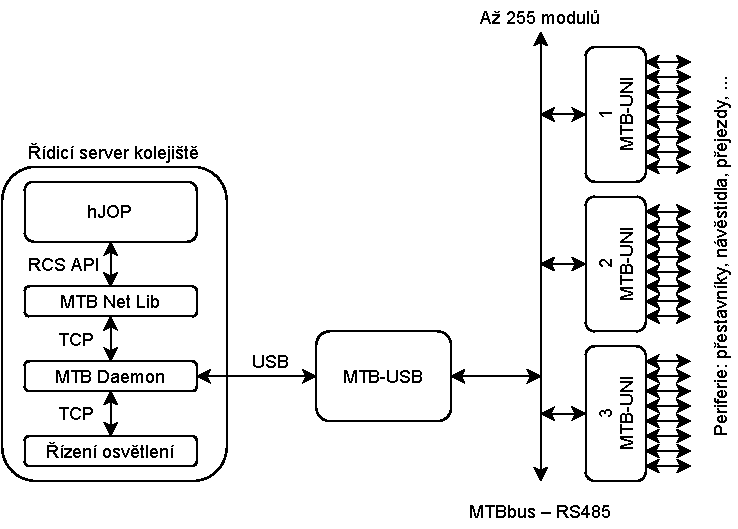
\includegraphics[width=0.8\textwidth]{data/new-topology.pdf}
\caption{Komponenty vytvořené v~rámci diplomové práce (mimo \textit{hJOP}
a~\textit{Řízení osvětlení}).}
\label{fig:new-topology}
\end{figure}

V~rámci práce byly formulovány požadavky (\ref{sub:mtbbus-req-summary}), které
má nový systém \gls{mtb} splnit. Všechny tyto požadavky byly naplněny.
Podařilo se vytvořit systém, který za poměrně malé finanční a časové náklady
značně povyšuje současný systém \gls{mtb}. Především však vznikl otevřený
a rozšiřitelný systém s~výhledem udržitelnosti po desítky let. Nový systém
\gls{mtb} umožní stavbu dalších kolejišť, udržování a rozšiřování kolejišť
současných. Nový systém \gls{mtb} si může vyrobit každý, kdo bude chtít bezpečně
řídit své modelové kolejiště.

Pro \gls{kmz} znamená \gls{mtb} v4 možnost nasadit více řídicích systémů
kolejiště, a~konečně tak zprovoznit řízení osvětlení, řízení tramvajové
a~autobusové dopravy. \gls{mtb} v4 umožní nasazení pultů obsluhy,
vytvoření nových chytrých zesilovačů \gls{dcc} signálu. Umožní výstavbu nového
depa kolejových vozidel, kde se budou používat speciální \gls{mtb} moduly.
Pro \gls{kmz} je \gls{mtb} v4 velkým krokem vpřed.

\gls{mtb} v4 bylo nasazeno na testovacím kolejišti o~20 modulech, kde úspešně
funguje.

\section{Možná rozšíření} \label{sec:future}

Při návrhu tak velkého systému, jako je \gls{mtb}, se přirozeně ukázaly mnohé
cesty, které by bylo možné v~budoucnu prozkoumat.

Systém \gls{mtb} by v~budoucnu mohl podporovat vyšší rychlosti komunikace nebo
automatickou detekci rychlosti sběrnice. \gls{mtb} by mohlo být rozšířeno
o~jednotky, které provádějí retranslaci dat sběrnice bezdrátově (pro vzdálené
připojení modulů).

Jednou z~otázek týkajících se budoucího rozšíření je, jak umožnit, aby systém
\gls{mtb} mohl interagovat s~komerčními softwary pro řízení modelových
kolejišť.
Dalším možným rozšířením je tak implementovat do majoritních komerčních
softwarů pro řízení modelových kolejišť podporu pro \gls{mtb}. Některé softwary
jsou však uzavřené. Pro takové softwary by bylo možné napsat alternativní
firmware do \gls{mtbusb}, který by zajistil, že \gls{mtbusb} modul se pro
počítač bude tvářit jako některý z~komerčních systémů pro řízení kolejišť.

Dalším přirozeným způsobem rozšíření, který má autor této práce v~plánu
v~nejbližším roce uskutečnit, je přidání dalších typů modulů. V~budoucnu
vzniknou \gls{mtb} moduly pro chytré zesilovače \gls{dcc} signálu,
\textit{RailCom} detektory a jiné. Systém \gls{mtb} je na tato rozšíření
připraven.


\printbibliography[heading=bibintoc]

\appendix
\chapter{Přílohy} \label{chap:appendix}
\vspace{-2em}

\begin{figure}[H]
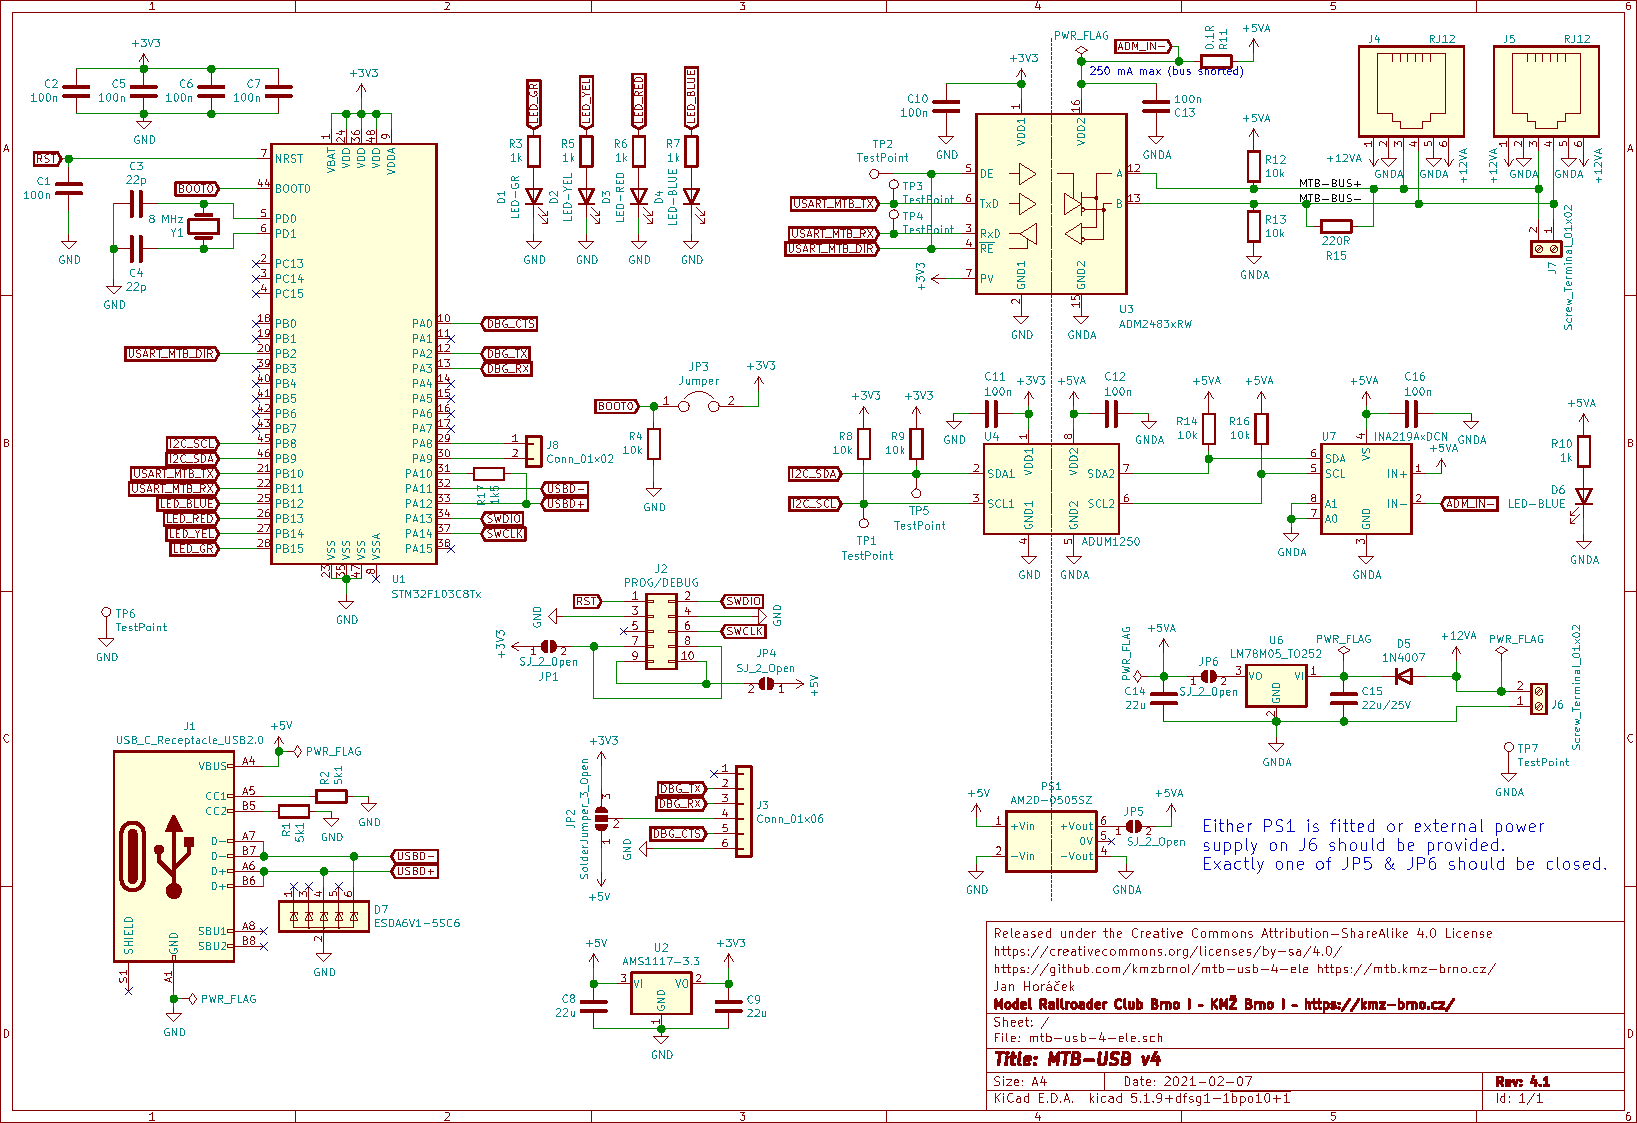
\includegraphics[angle=90,width=\textwidth]{data/mtb-usb-4-ele.pdf}
\caption{Schéma \gls{mtbusb} modulu.}
\label{fig:mtb-usb-sch}
\end{figure}

\begin{figure}[ht]
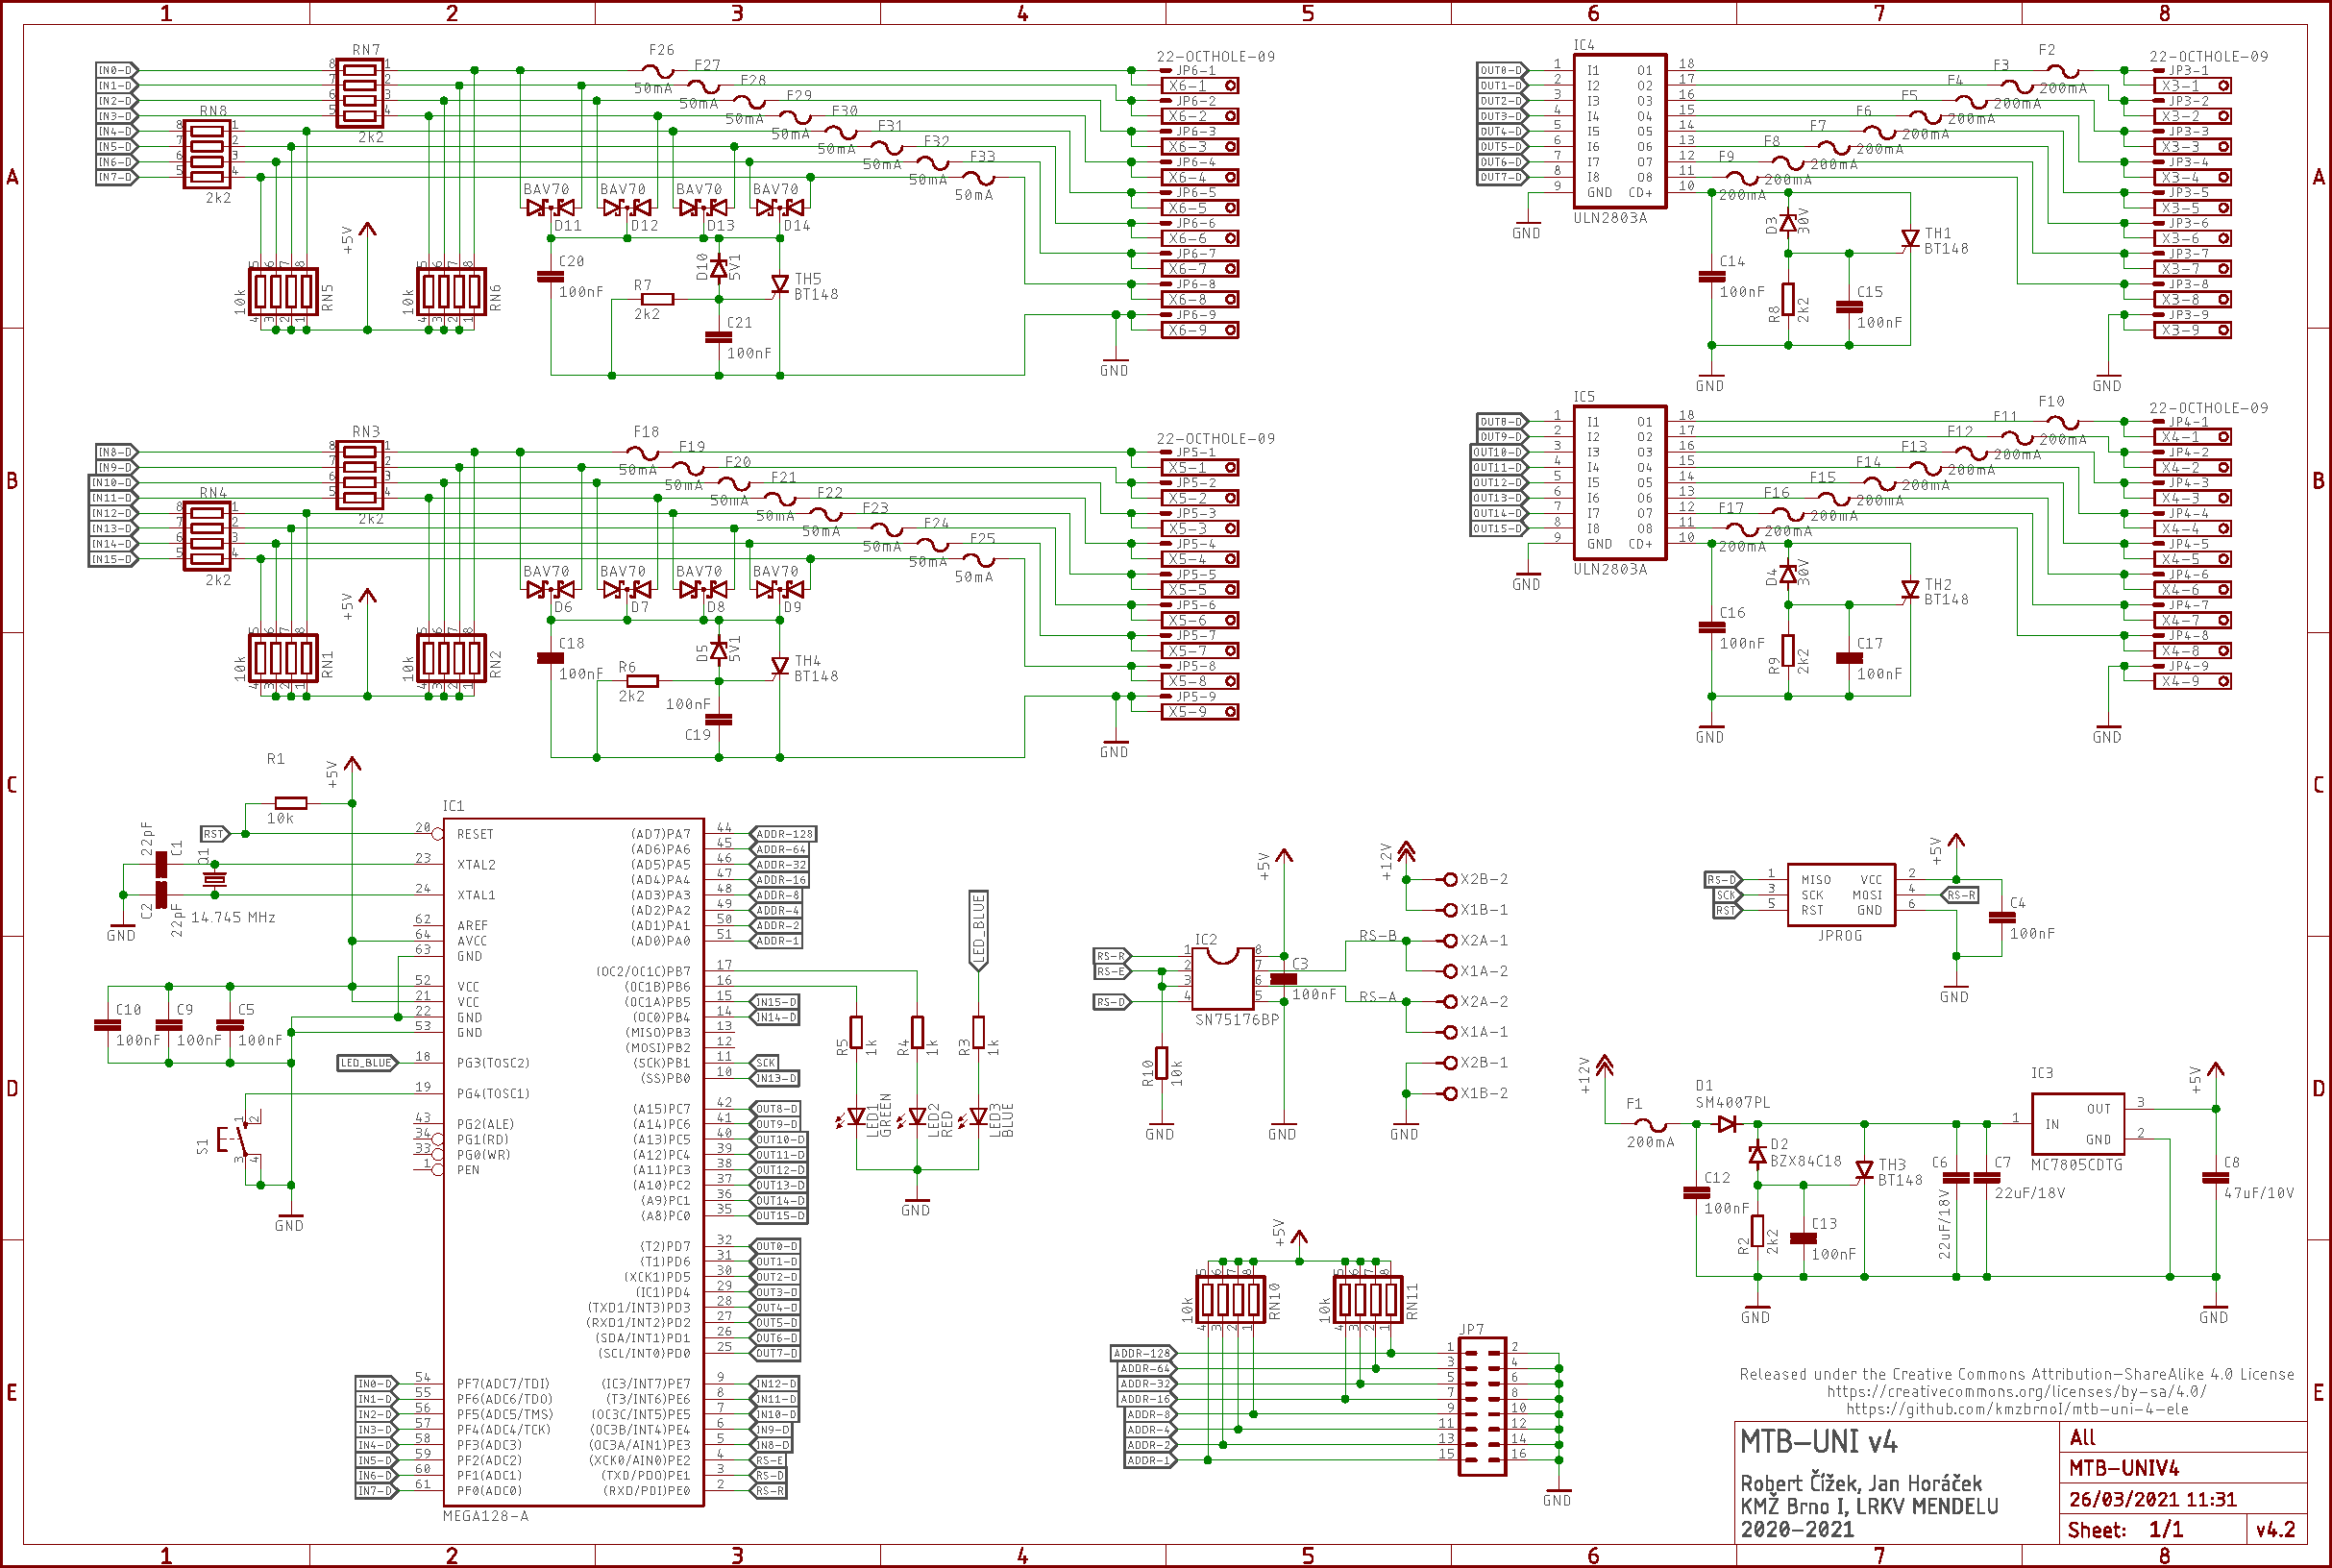
\includegraphics[angle=90,width=\textwidth]{data/mtb-uni-4-ele.pdf}
\caption{Schéma \gls{mtbuni} v4 modulu.}
\label{fig:mtb-uni-4-sch}
\end{figure}

\begin{figure}[ht]
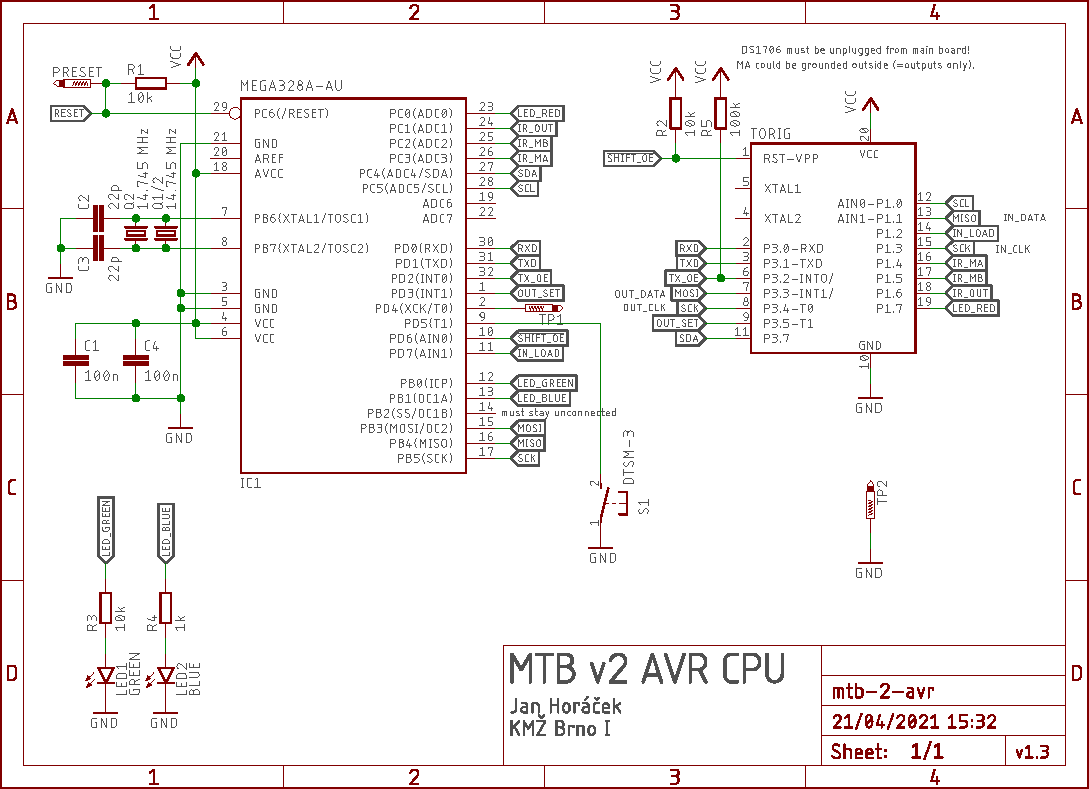
\includegraphics[angle=90,width=\textwidth]{data/mtb-2-avr-ele.pdf}
\caption{Schéma nástavné desky \textit{MTB-2-AVR}.}
\label{fig:mtb-uni-2-avr-sch}
\end{figure}

\begin{figure}[ht]
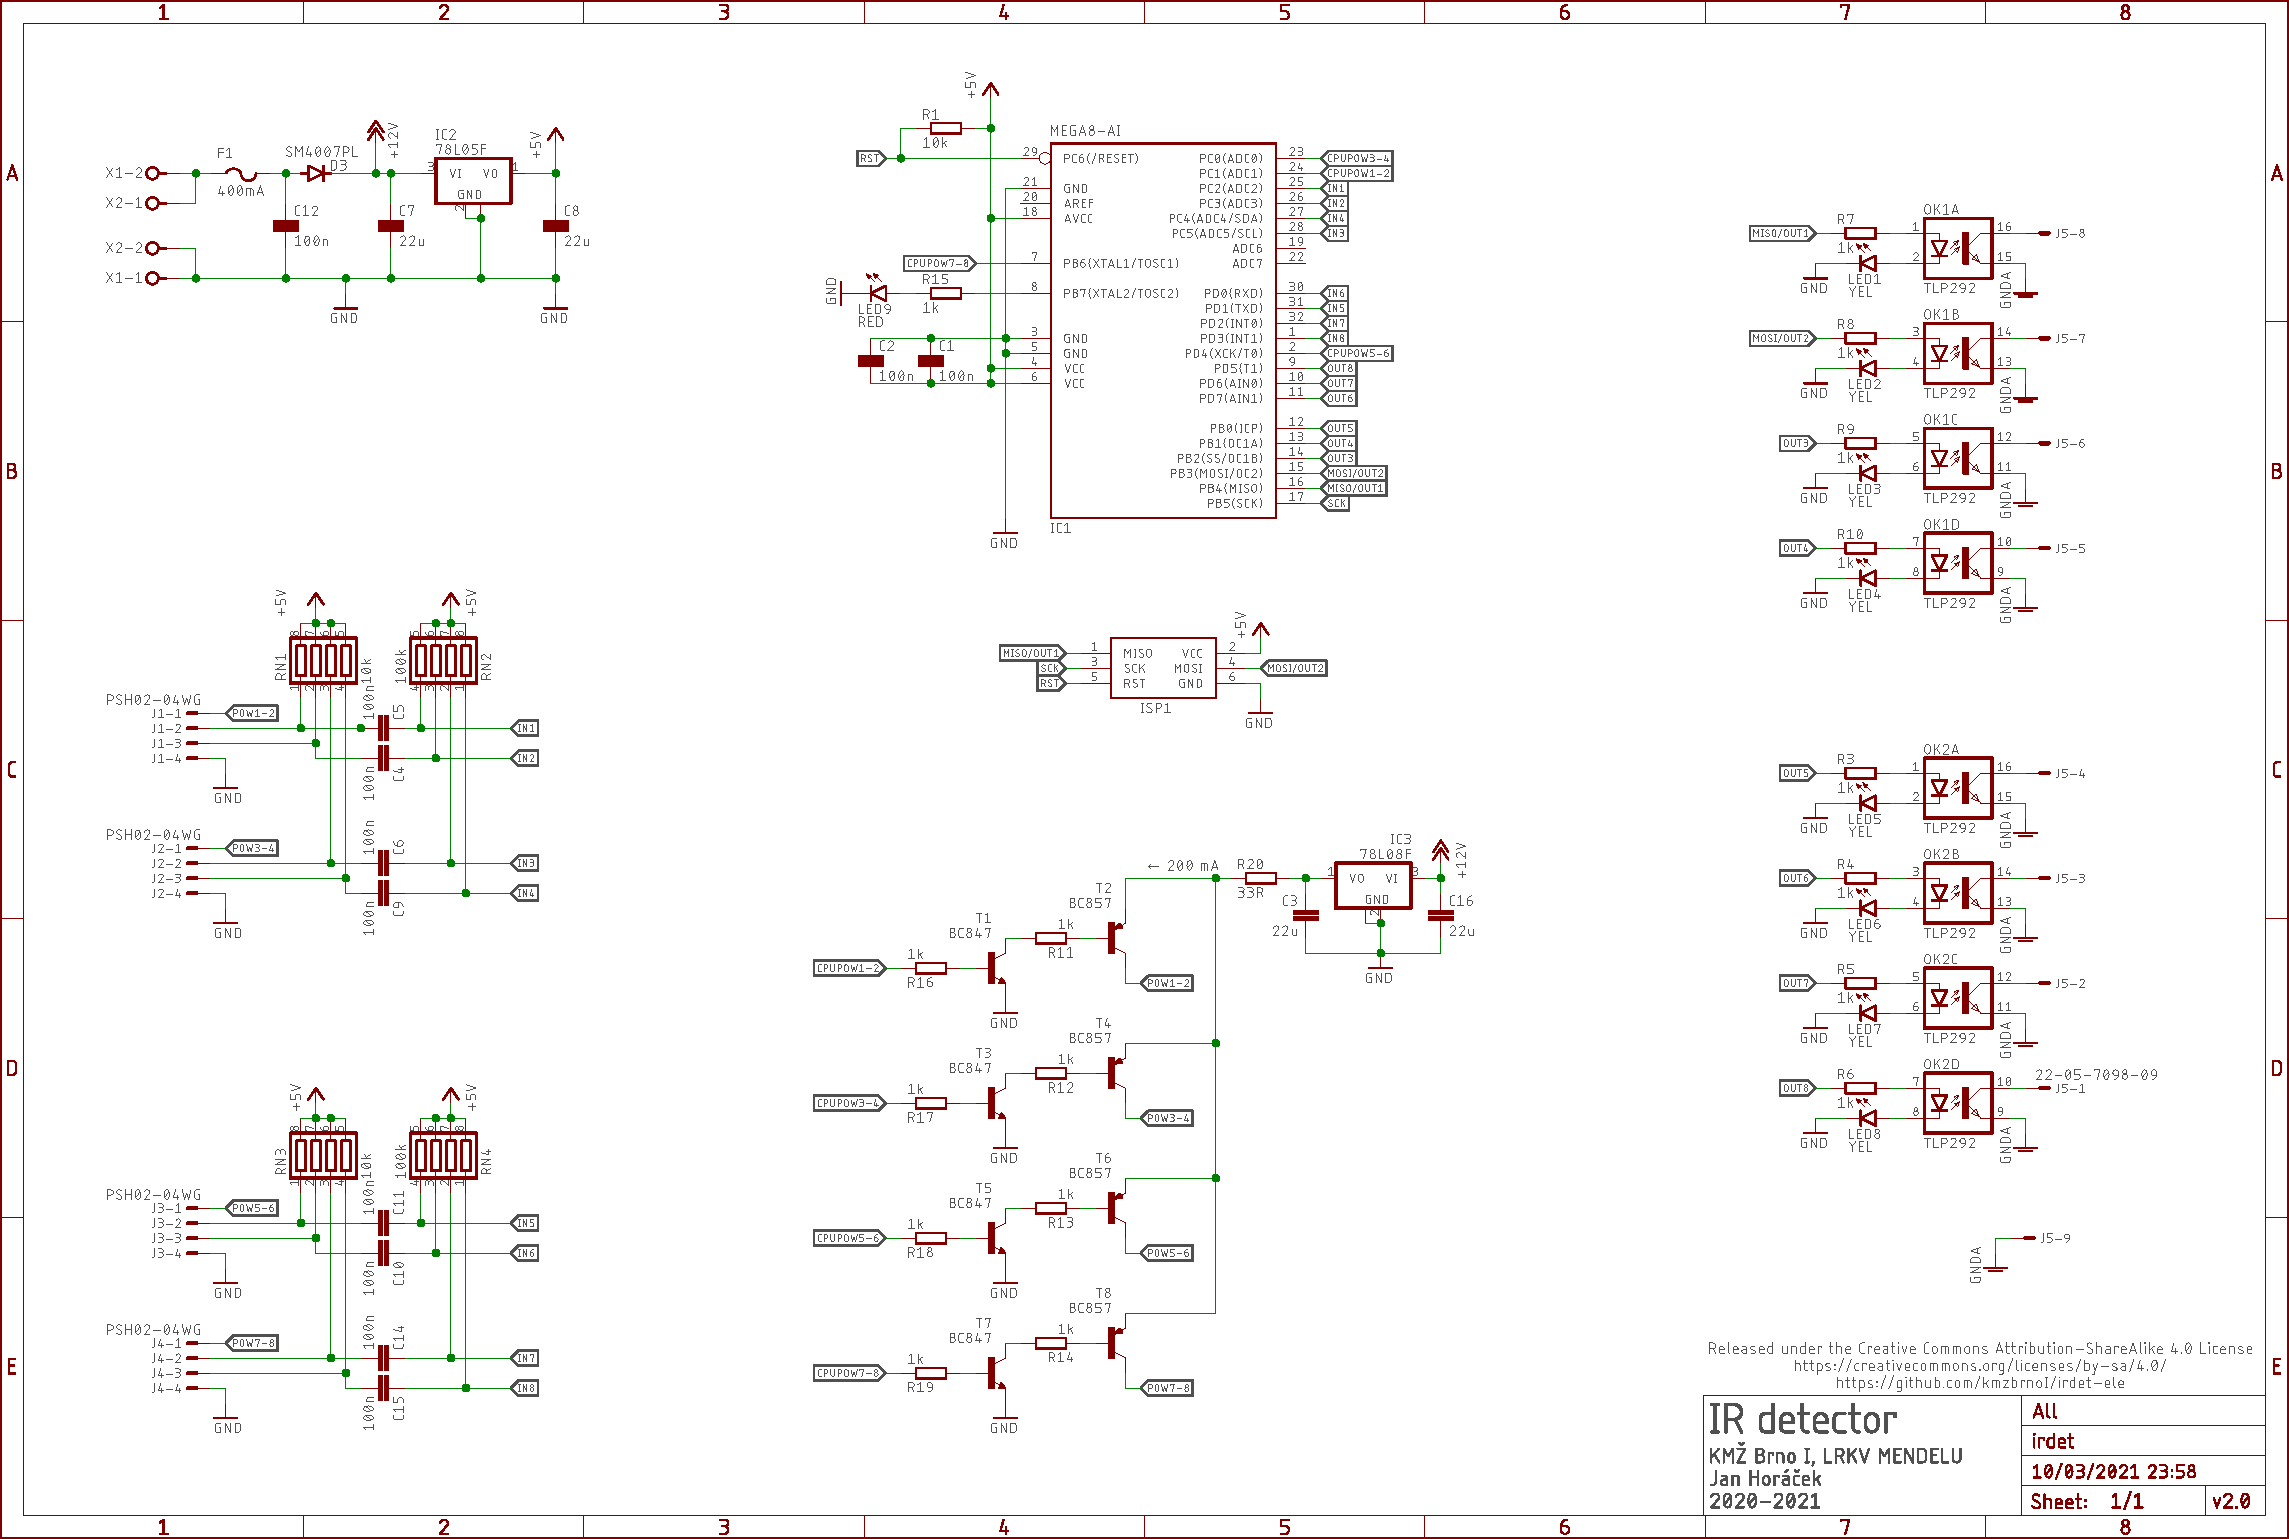
\includegraphics[angle=90,width=\textwidth]{data/irdet-ele.pdf}
\caption{Schéma desky \textit{IRdet}.}
\label{fig:irdet-sch}
\end{figure}


\end{document}
